
\documentclass[a4paper,11pt]{book}
\usepackage[utf8]{inputenc}
\usepackage{lmodern}
\usepackage{verbatim}
\usepackage{graphicx}
\usepackage{amsmath}
\usepackage{amssymb}
\usepackage{amsthm}
\usepackage{tabularx}
\usepackage{multirow}
\usepackage{multicol}
\usepackage{fancyvrb}
\usepackage{float}
\usepackage{listings}
\usepackage[svgnames]{xcolor}
\usepackage{array}
\usepackage{booktabs}
\usepackage{siunitx}
\usepackage{times}
\usepackage{subcaption}
\usepackage{mathtools}
\usepackage{microtype}
\usepackage{tcolorbox}
\usepackage{newverbs}

\usepackage{listings}

\usepackage[
    type={CC},
    modifier={by-nc-sa},
    version={4.0},
]{doclicense}

\usepackage{wrapfig}
\usepackage{geometry}

\definecolor{mylightblue}{RGB}{186,191,255}
\definecolor{mystrongblue}{RGB}{78,90,255}
\definecolor{graytitle}{gray}{0.5}
\definecolor{cverbbg}{gray}{0.93}

\definecolor{titlepagecolor}{RGB}{10,10,10}

\usepackage[colorlinks,
            linkcolor=mystrongblue,
            anchorcolor=mystrongblue,
            citecolor=mystrongblue,
            urlcolor=mystrongblue]{hyperref}

\newenvironment{cverbatim}
 {\SaveVerbatim{cverb}}
 {\endSaveVerbatim
  \flushleft\fboxrule=0pt\fboxsep=.5em
  \colorbox{cverbbg}{\BUseVerbatim{cverb}}%
  \endflushleft
}

\newenvironment{lcverbatim}
 {\SaveVerbatim{cverb}}
 {\endSaveVerbatim
 \footnotesize
 \sffamily
 % \texttt{
  \flushleft\fboxrule=0pt\fboxsep=.5em
  \colorbox{cverbbg}{%
    \makebox[\dimexpr\linewidth-2\fboxsep][l]{\BUseVerbatim{cverb}}%
 % }
 }
  \endflushleft
}

%\lstset{frame=single,
%  language=C++,
%  aboveskip=3mm,
%  belowskip=3mm,
%  showstringspaces=false,
%  columns=flexible,
%  basicstyle={\small\ttfamily},
%  numbers=none,
%  numberstyle=\tiny\color{gray},
%  keywordstyle=\color{blue},
%  commentstyle=\color{dkgreen},
%  stringstyle=\color{mauve},
%  breaklines=true,
%  breakatwhitespace=true,
%  tabsize=3,
%  captionpos=b
%}

\newenvironment{dedication}
{
   \cleardoublepage
   \thispagestyle{empty}
   \vspace*{\stretch{1}}
   \hfill\begin{minipage}[t]{0.66\textwidth}
   \raggedright
}
{
   \end{minipage}
   \vspace*{\stretch{3}}
   \clearpage
}

\makeatletter
\renewcommand{\@chapapp}{}
\newenvironment{chapquote}[2][2em]
  {\setlength{\@tempdima}{#1}
   \def\chapquote@author{#2}
   \parshape 1 \@tempdima \dimexpr\textwidth-2\@tempdima\relax%
   \itshape}
  {\par\normalfont\hfill--\ \chapquote@author\hspace*{\@tempdima}\par\bigskip}
\makeatother

\title{\Huge \textbf{LAMMPS tutorials}}
\author{\textsc{Simon Gravelle}}
\date{}

\begin{document}

\thispagestyle{empty}
\setcounter{page}{0}

\noindent {\Huge LAMMPS tutorials}

\noindent {\large First edition}

\vspace{1.5cm}

%\noindent This work is licensed under the \href{http://creativecommons.org/licenses/by/4.0/}{Creative Commons 
%Attribution 4.0 International License}.

\doclicenseThis

\vspace{1.5cm}

\noindent \textbf{\large You are free to:}

\vspace{0.25cm}

\noindent  \textbf{Share} — copy and redistribute the material in any medium or format for any purpose, even commercially.

\vspace{0.1cm}

\noindent  \textbf{Adapt} — remix, transform, and build upon the material for any purpose, even commercially. The licensor cannot revoke these freedoms as long as you follow the license terms.

\vspace{0.5cm}
\noindent \textbf{\large Under the following terms:}

\vspace{0.25cm}
 
\noindent \textbf{Attribution} — You must give appropriate credit , provide a link to the license, and indicate if changes were made . You may do so in any reasonable manner, but not in any way that suggests the licensor endorses you or your use.

\vspace{0.1cm}

\noindent \textbf{No additional restrictions} — You may not apply legal terms or technological measures that legally restrict others from doing anything the license permits.


\tableofcontents
%\listoffigures
%\listoftables
\mainmatter

\include{non-tutorials/before-you-start.tex}
\chapter{Lennard Jones fluid}

\vspace{-1cm} \noindent \textcolor{graytitle}{\textit{{\Large The very basics of LAMMPS through a simple example}}\vspace{0.5cm} }

\noindent \hspace{-0.45cm}\begin{wrapfigure}{r}{4cm}
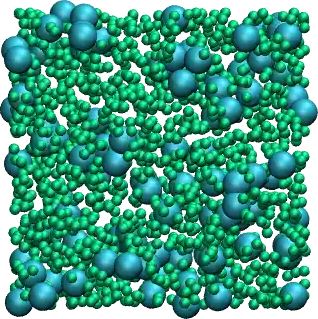
\includegraphics[width=4cm]{tutorials/level0/lennard-jones-fluid/binary_LJ_fluid_light.png}
\end{wrapfigure}

\noindent The objective of this tutorial is to use
LAMMPS to perform a simple molecular dynamics simulation
of a binary fluid in the NVT ensemble. The system is a simple Lennard-Jones fluid
made of neutral dots with a Langevin thermostating. The
simulation box is cubic with periodic boundary conditions.
This tutorial illustrates the use of several ingredients of
molecular dynamics simulations, such as system initialization,
energy minimization, integration of the equations of motion,
and trajectory visualization.

\section{Required softwares}

\noindent Download and install LAMMPS by following the instructions of the \href{https://lammps.sandia.gov}{LAMMPS website}.
Alternatively, if you are using Ubuntu OS, you can simply execute the
following command in a terminal:

\begin{lcverbatim}
sudo apt-get install lammps
\end{lcverbatim}

\noindent You can verify that LAMMPS is indeed installed on your
computer by typing in a terminal :

\begin{lcverbatim}
lmp
\end{lcverbatim}

\noindent You should see the version of LAMMPS that has been
installed. On my computer I see

\begin{lcverbatim}
LAMMPS (29 Sep 2021 - Update 2)
\end{lcverbatim}

\noindent In addition to LAMMPS, you will also need \href{https://help.gnome.org/users/gedit/stable/}{(1) a basic text editing software}
such as Vim, Gedit, or Notepad++, \href{https://www.ks.uiuc.edu/Research/vmd/}{(2) a visualization software}, here I
will use VMD (note: VMD is free but you have to register to
the uiuc website in order to download it. If you don't want
to, you can also use Ovito.), \href{https://plasma-gate.weizmann.ac.il/Grace/}{(3) a plotting tool} like
XmGrace or pyplot.

\section{The input script}

\noindent In order to run a simulation using LAMMPS, one needs to
write a series of commands in an input script. For clarity,
this script will be divided into five categories which we are going to
fill up one by one. Create a blank text file, call it
\textit{input1.lammps}, and copy the following lines in it:

\begin{lcverbatim}
# PART A - ENERGY MINIMIZATION
# 1) Initialization
# 2) System definition
# 3) Simulation settings
# 4) Visualization
# 5) Run
\end{lcverbatim}

\noindent These five categories are not required in every
input script, and should not necessarily be in that
exact order. For instance parts 3 and 4 could be inverted, or
part 4 could be omitted, or there could be several
consecutive runs.
A line starting with a brace ($\#$) is a comment
that is ignored by LAMMPS. Use comments to structure 
your inputs and make them readable by others.

\subsection{System creation}

\noindent In the first section of the script, called \textit{Initialization},
let us indicate to LAMMPS the type of simulation we are
going to execute by specifying the most basic information,
such as the conditions at the boundaries of the box (i.e.
periodic, non-periodic) or the type of atoms (e.g. uncharged
single dots, spheres with angular velocities). Enter the
following lines:

\begin{lcverbatim}
# 1) Initialization
units lj
dimension 3
atom_style atomic
pair_style lj/cut 2.5
boundary p p p
\end{lcverbatim}

\noindent The first line indicates that we want to
use the system of unit called \textit{LJ}, for Lennard-Jones, for which all quantities
are unitless. 

\begin{tcolorbox}[colback=mylightblue!5!white,colframe=mylightblue!75!black,title=Background Information -- About LJ units]
Lennard-Jones (LJ) units are a dimensionless system of units that are often used in molecular simulations
and theoretical calculations. When using LJ units:
\begin{itemize}
\item energies are expressed in units of $\epsilon$, where $\epsilon$ is the
  depth of the potential of the LJ interaction,
\item distances are expressed in units of $\sigma$, where $\sigma$ is the distance
  at which the particle-particle potential energy is zero,
\item masses are expressed in units of the atomic mass $m$.
\end{itemize}
All the other quantities are normalized by a combination of $\epsilon$, $\sigma$,
and $m$. For instance, time is expressed in units of $\sqrt{ \epsilon / m \sigma^2}$. 
\end{tcolorbox}

\noindent The second line indicates that the simulation
is 3D, the third line that the \textit{atomic} style
will be used, therefore each atom is just a dot with a mass.

\begin{tcolorbox}[colback=mylightblue!5!white,colframe=mylightblue!75!black,title=About the atom style]
While we are keeping it simple here,
in the following tutorials, different \textit{atom$\_$style} will be used,
allowing us to create atoms with a net charge and to define 
bonds between atoms to form molecules.
\end{tcolorbox}

\noindent The fourth line indicates that atoms are going to interact
through a Lennard-Jones potential with a cut-off equal to
2.5 (unitless), and the last line indicates that the
periodic boundary conditions will be used along all three
directions of space (the 3 \textit{p} stand for \textit{x}, \textit{y}, and \textit{z},
respectively).
At this point, you have a LAMMPS script that does nothing.
You can execute it to verify that there is no mistake by
running the following command in the terminal:

\begin{lcverbatim}
lmp -in input_01.lammps
\end{lcverbatim}

\noindent Which should return something like

\begin{lcverbatim}
LAMMPS (29 Sep 2021 - Update 2)
Total wall time: 0:00:00
\end{lcverbatim}

\noindent If there is a mistake in the input script, for example if
\textit{atom$\_$stile} is written instead of \textit{atom$\_$style}, LAMMPS
gives you an explicit warning:

\begin{lcverbatim}
LAMMPS (29 Sep 2021 - Update 2)
ERROR: Unknown command: atom_stile  atomic (src/input.cpp:232)
Last command: atom_stile atomic
\end{lcverbatim}

\noindent Let us fill the second part the of the input script:

\begin{lcverbatim}
# 2) System definition
region simulation_box block -20 20 -20 20 -20 20
create_box 2 simulation_box
create_atoms 1 random 1500 341341 simulation_box
create_atoms 2 random 100 127569 simulation_box
\end{lcverbatim}

\noindent The first line creates a region of space
named \textit{simulation$\_$box} that is a block (a rectangular cuboid) and
extends from -20 to 20 along all 3 directions of space, all expressed in
non-dimensional units because we are using the LJ system
of units. The second line creates a simulation box based on
the region \textit{simulation$\_$box} with \textit{2} types of atoms. The third
command specifies that 1500 atoms of type 1 must be created
randomly in the region \textit{simulation$\_$box}. The integer \textit{341341} is a
seed that can be changed in order to create different
initial conditions for the simulation. The fourth line
creates 100 atoms of type 2.
If you run LAMMPS, you should see the following in the
terminal:

\begin{lcverbatim}
LAMMPS (29 Sep 2021 - Update 2)
Created orthogonal box = (-20 -20 -20) to (20 20 20)
1 by 1 by 1 MPI processor grid
Created 1500 atoms
using lattice units in orthogonal box = (-20 -20 -20) to (20 20 20)
create_atoms CPU = 0.001 seconds
Created 100 atoms
using lattice units in orthogonal box = (-20 -20 -20) to (20 20 20)
create_atoms CPU = 0.000 seconds
Total wall time: 0:00:00
\end{lcverbatim}

\noindent From what is printed in the terminal, it is clear that
LAMMPS correctly interpreted the commands, and first created
the box with desired dimensions, then 1500 atoms, then 100
atoms.
Let us fill the third section of the input script, the settings:

\begin{lcverbatim}
# 3) Simulation settings
mass 1 1
mass 2 1
pair_coeff 1 1 1.0 1.0
pair_coeff 2 2 0.5 3.0
\end{lcverbatim}

\noindent The two first commands attribute a mass
equal to 1 (unitless) to both atoms of type 1 and 2,
respectively. The third line sets the Lennard-Jones
coefficients for the interactions between atoms of type 1,
respectively the depth of the potential well
$\epsilon$ and the distance at which the
particle-particle potential energy is zero $\sigma$. 
The last line sets the Lennard-Jones coefficients for
the interactions between atoms of type 2.

\begin{tcolorbox}[colback=mylightblue!5!white,colframe=mylightblue!75!black,title=About cross parameters]
By default, LAMMPS calculates the cross coefficients between the different atom types
using geometric average: 
$\epsilon_{ij} = \sqrt{\epsilon_{ii} \epsilon_{jj}}$,
$\sigma_{ij} = \sqrt{\sigma_{ii} \sigma_{jj}}$. 
In the present case, and even without specifying it explicitly, we thus have:
\begin{itemize}
\item $\epsilon_{ij} = \sqrt{1.0 \times 0.5} = 0.707$, and 
\item $\sigma_{ij} = \sqrt{1.0 \times 3.0} = 1.732$.
\end{itemize}
Eventually, cross parameters could also be explicitly specified by adding the following 
line to the input file (but there is no need to do it here, its only necessary if you need 
to set custom parameters):
\begin{lcverbatim}

pair_coeff 1 2 0.707 1.732 
\end{lcverbatim}

\noindent Note that the arithmetic rule, where 
$\epsilon_{ij} = \sqrt{\epsilon_{ii} \epsilon_{jj}}$,
$\sigma_{ij} = (\sigma_{ii}+\sigma_{jj})/2$, 
is more common than the geometric rule. However, neither the geometric nor the
arithmetic rule are based on rigorous argument, so here
the geometric rule will do just fine. 
\end{tcolorbox}

\noindent \subsection{Energy minimization}

Now that the system is fully defined, let us just fill the two last remaining sections:

\begin{lcverbatim}
# 4) Visualization
thermo 10
# 5) Run
minimize 1.0e-4 1.0e-6 1000 10000
\end{lcverbatim}

\noindent The thermo command asks LAMMPS to print
thermodynamic information (e.g. temperature, energy) in the
terminal every 10 steps. The second line asks LAMMPS to
perform an energy minimization of the system.

\begin{tcolorbox}[colback=mylightblue!5!white,colframe=mylightblue!75!black,title=About energy minimization]
An energy minimization procedure consists in adjusting
the coordinates of the atoms that are too close from one another until one of the stopping
criteria is reached. By default, LAMMPS uses the conjugate gradient (CG) algorithm.
Here there are four stopping criteria:
\begin{itemize}
\item The change in energy between two iterations is less than 1.0e-4,
\item The maximum force between two atoms in the system is lower than 1.0e-6,
\item The maximum number of iterations is 1000,
\item The maximum number of times the force and the energy have been evaluated is 10000.
\end{itemize}
\end{tcolorbox}

\noindent Now running the simulation, we can see how the thermodynamics
variables evolve with time:

\begin{lcverbatim}
Step Temp         E_pair  E_mol       TotEng         Press
0       0       78840982      0     78840982       7884122 
10      0      169.90532      0    169.90532     17.187291 
20      0    -0.22335386      0  -0.22335386 -0.0034892297 
30      0    -0.31178296      0  -0.31178296 -0.0027290466 
40      0    -0.38135002      0  -0.38135002 -0.0016419218 
50      0    -0.42686621      0  -0.42686621 -0.0015219081 
60      0    -0.46153953      0  -0.46153953 -0.0010659992 
70      0    -0.48581568      0  -0.48581568 -0.0014849169 
80      0    -0.51799572      0  -0.51799572 -0.0012995545 
\end{lcverbatim}

\noindent These lines give us information concerning
the progress of the energy minimization. First, at the start
of the simulation (step 0), the energy in the system is
huge: 78840982 (unitless). This was expected because
the atoms have been created at random positions within the
simulation box, and some of them are probably overlapping,
resulting in a large initial energy which is the consequence
of the repulsive part of the Lennard-Jones interaction
potential. As the energy minimization progresses, the energy
rapidly decreases and reaches a negative value, indicating that the atoms have been
displaced at reasonable distances from one another. Other
useful information have been printed in the terminal, for
example, LAMMPS tells us that the first of the four criteria
to be satisfied was the energy:

\begin{lcverbatim}
Minimization stats:
Stopping criterion = energy tolerance
\end{lcverbatim}

\noindent \subsection{Molecular dynamics}

\begin{tcolorbox}[colback=mylightblue!5!white,colframe=mylightblue!75!black,title=Background Information -- What is molecular dynamics?]
Molecular dynamics (MD) is based on the numerical solution of the Newtonian
equations of motion for every atom $i$,
$$\sum_{j \ne i} \boldsymbol{F}_{ji} = m_i \times \boldsymbol{a}_i,$$
where $\sum$ is the sum over all the atoms other than $i$, 
$\boldsymbol{F}_{ji}$ the force between the atom pairs $j-i$,
$m_i$ the mass of atom $i$, and $\boldsymbol{F}_i$ its acceleration. 
The Newtonian equations are solved every timestep to predict the
evolution of the positions and velocities of atoms and molecules over time. 

At every timestep, the following operations usually occur when 
performing a MD simulation:
\begin{itemize}
\item the forces between the atoms are calculated from the parameters (here the $\epsilon$ and $\sigma$ values) and potentials (here Lennard-Jones),
\item the acceleration of each atom is evaluated from the Newtonian equation,
\item the velocity and position of each atom are updated according to the acceleration, typically using the Verlet algorithm, or similar.
\end{itemize}
\end{tcolorbox}

\noindent The system is now ready. Let us continue filling up the
input script and adding commands in order to perform an actual molecular dynamics
simulation that will start from the final state of the energy minimization.
In the same input script, after the \textit{minimization} command, add the following
lines:

\begin{lcverbatim}
# PART B - MOLECULAR DYNAMICS
# 4) Visualization
thermo 1000
variable kinetic_energy equal ke
variable potential_energy equal pe
variable pressure equal press
fix myat1 all ave/time 10 1 10 v_kinetic_energy v_potential_energy file energy.dat
# 5) Run
fix mynve all nve
fix mylgv all langevin 1.0 1.0 0.1 1530917
timestep 0.005
run 10000
\end{lcverbatim}

\noindent Since LAMMPS reads the input from top to
bottom, these lines will be executed after the energy
minimization. There is no need to (re-)initialize the system
(part 1), (re-)define it (part 2), or (re-)specify the settings
(part 3). The \textit{thermo} command is called a second time within the 
same input, so the previously entered value of \textit{10} will be replaced
by the value of \textit{1000} as soon as the second run starts.

Three variables have been defined in order
to print the kinetic energy and the potential energy 
of the system in the file named \textit{energy.dat}. Then,
in the run section, the fix \textit{nve} is used to update the
positions and the velocities of the atoms in the group
\textit{all} (this is the most important command here). The second
fix applies a Langevin thermostat to the atoms of group
\textit{all}, with a desired temperature of 1 and a damping
parameter of 0.1. The number \textit{1530917} is a seed, you can
change it to perform statistically independent simulations
with the same system. Finally we choose the timestep
and we ask LAMMPS to run for 10000 steps. After running
the simulation, you should see the following information in
the terminal:

\begin{lcverbatim}
Step         Temp       E_pair    E_mol       TotEng        Press
1000    0.9880227  -0.31773089        0    1.1633769  0.021818374 
2000    1.0434396  -0.26534383        0    1.2988374   0.02287591 
3000   0.97269039  -0.23946371        0      1.21866  0.022394592 
4000    1.0192798  -0.23174747        0    1.2962167  0.024978385 
5000    1.0319547  -0.23284134        0    1.3141233  0.024342347 
6000   0.98137972  -0.22477315        0    1.2463764  0.022074749 
7000    1.0144842  -0.23803792        0    1.2827372  0.023846178 
8000    1.0102062  -0.23305477        0    1.2813075     0.023146 
9000    1.0236358  -0.22539436        0    1.3090996  0.024357378 
\end{lcverbatim}

\noindent The second column shows that the temperature
starts from 0, but rapidly reaches the
expected value near $T=1$, as requested. 
Note that  In the terminal, you may also see

\begin{lcverbatim}
Total (number) of neighbors = 8560
Ave neighs/atom = 5.35
Neighbor list builds = 999
Dangerous builds = 998
Total wall time: 0:00:02
\end{lcverbatim}

\noindent Note: If you see \textit{Dangerous builds = 0}, as could be
the case with some LAMMPS versions, you can ignore
the next part.
During the simulation, they have been 998 dangerous builds.
This is an indication that something is wrong: some atoms
have moved more than expected in between two calculations of
the neighbor lists. Let us add the following command in the
\textit{Simulation settings} section:

\begin{lcverbatim}
neigh_modify every 1 delay 5 check yes
\end{lcverbatim}

\noindent With this command, LAMMPS will rebuild the neighbor lists
more often. Re-run the simulation, and you should see a more
positive outcome with 0 dangerous build:

\begin{lcverbatim}
Total (number) of neighbors = 2024
Ave neighs/atom = 1.2650000
Neighbor list builds = 1253
Dangerous builds = 0
Total wall time: 0:00:02
\end{lcverbatim}

\noindent From what has been printed in the energy.dat file, let us
plot the potential energy and the pressure of
the system over time:

\begin{figure}
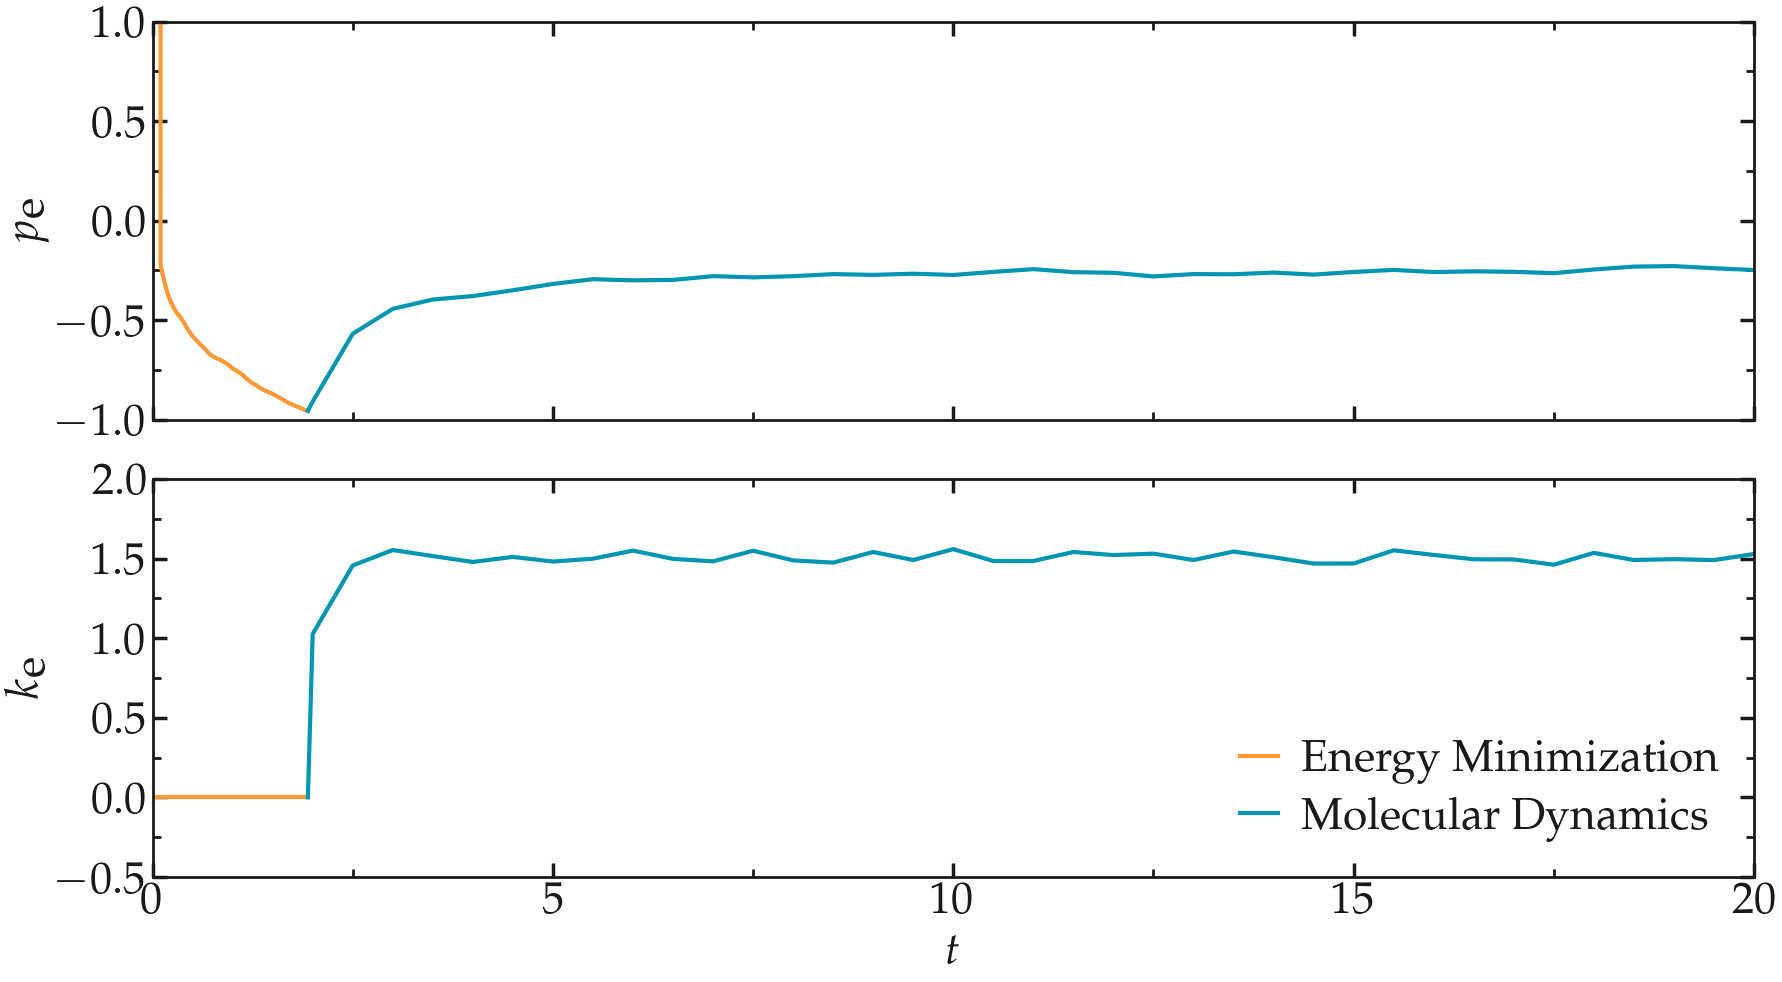
\includegraphics[width=\linewidth]{tutorials/level0/lennard-jones-fluid/energy-light.png}
\end{figure}

\begin{tcolorbox}[colback=mylightblue!5!white,colframe=mylightblue!75!black,title=On the necessity of plotting data efficiently]
When testing/debugging a molecular simulation, it is crucial to be able to control 
on-the-fly the outputs such as the energy to make sure the
system is behaving as expected. If you don't already have 
a favorite plotting tool, you can use xmgrace and simply type from the terminal:
\begin{lcverbatim}
xmgrace energy.dat
\end{lcverbatim}

\noindent This command will automatically plot the second column as a function of the first column.
Here I am using pyplot for esthetic reason. If you want, you can download the Jupyter-notebook
from the \href{https://github.com/lammpstutorials/lammpstutorials.github.io/tree/version2.0/docs/inputs}{the inputs folder} repository (in the \textit{level0/lennard-jones-fluid/} folder).
\end{tcolorbox}

\noindent \section{Trajectory visualisation}

\hspace{-0.45cm}\begin{wrapfigure}{r}{4cm}
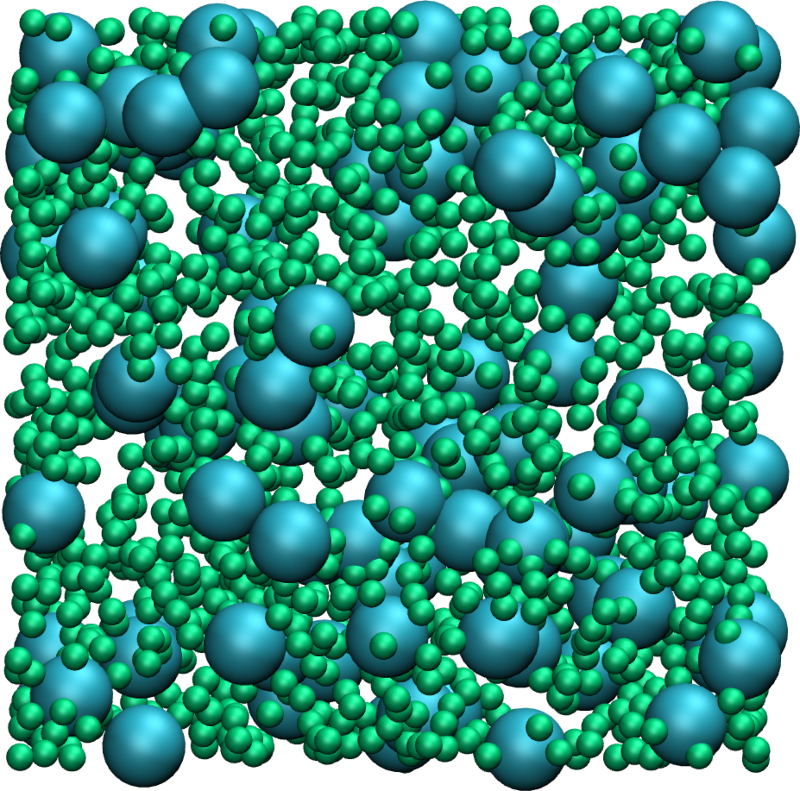
\includegraphics[width=4cm]{tutorials/level0/lennard-jones-fluid/input1.png}
\end{wrapfigure}

\noindent The simulation is running well, but we would like to
visualize the trajectories of the atoms. To do so, we need
to dump the positions of the atoms in a file at a regular
interval. Add the following command in the \textit{visualization}
section of PART B:

\begin{lcverbatim}
dump mydmp all atom 1000 dump.lammpstrj
\end{lcverbatim}

\noindent Run LAMMPS again. A file named \textit{dump.lammpstrj} must appear in
the same folder as your input. This file can be opened using
VMD or Ovito. In Ubuntu, if VMD is installed, you can simply
execute in the terminal:

\begin{lcverbatim}
vmd dump.lammpstrj
\end{lcverbatim}

\noindent Otherwise, you can open VMD and import the \textit{dump.lammpstrj}
file manually using file $\rightarrow$ molecule. You should see a cloud
of lines, but you can improve the representation and make it
look like the figure on the right, or the video at the 
top of this page. 

\section{Improving the script}

\noindent Let us improve the input script and perform slightly more
advanced operations.

\hspace{-0.45cm}\begin{wrapfigure}{r}{4cm}
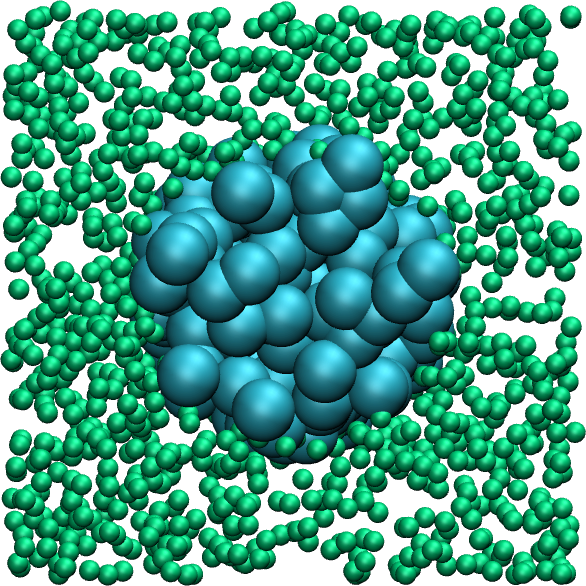
\includegraphics[width=4cm]{tutorials/level0/lennard-jones-fluid/input2.png}
\end{wrapfigure}

\noindent \subsection{Control the initial atom positions}

Let us create the atoms of type 1 and 2 in two separate
regions, respectively, instead of creating them both randomly 
within the entire space as we did previously. Create a new input script, and call
it \textit{input2.lammps}. Similarly to what has been done previously, copy the following lines
into the input script:

\begin{lcverbatim}
# 1) Initialization
units lj
dimension 3
atom_style atomic
pair_style lj/cut 2.5
boundary p p p
\end{lcverbatim}

\noindent Let us create a box from a predefined region,
and create two additional regions and generate
atoms of type 1 and 2 in each region respectively.

\begin{lcverbatim}
# 2) System definition
region simulation_box block -20 20 -20 20 -20 20
create_box 2 simulation_box
region mycylin cylinder z 0 0 10 INF INF side in
region mycylou cylinder z 0 0 10 INF INF side out
create_atoms 1 random 1000 341341 mycylou
create_atoms 2 random 150 127569 mycylin
\end{lcverbatim}

\noindent The \textit{side in} and \textit{side out} keywords
allow us to define regions that are respectively inside the
cylinder, and everything that is not inside the cylinder.
We can write the remaining of the input script as follow:

\begin{lcverbatim}
# 3) Simulation settings
mass 1 1
mass 2 1
pair_coeff 1 1 1.0 1.0
pair_coeff 2 2 0.5 3.0
neigh_modify every 1 delay 5 check yes
# 4) Visualization
thermo 10
dump mydmp all atom 10 dump.min.lammpstrj
# 5) Run
minimize 1.0e-4 1.0e-6 1000 10000
write_data minimized_coordinate.data
\end{lcverbatim}

\noindent The novelty with respect to the previous
input script is the command \textit{write$\_$data}. This command
asks LAMMPS to print the final state of the simulation in
a file named \textit{minimized$\_$coordinate.data}. This file will
be used later to restart the simulation from the final
state of the energy minimisation step.
Run LAMMPS using the \textit{input2.lammps} script. If everything
goes well, a dump file named \textit{dump.min.lammpstrj} will
appear in the folder, allowing you to visualize the atoms
trajectories during minimization. In
addition, a file named \textit{minimized$\_$coordinate.data} will be
created. If you open this file, you will see that it
contains all the information necessary to restart the
simulation, such as the number of atoms and the size of
the box:

\begin{lcverbatim}
1150 atoms
2 atom types
-20 20 xlo xhi
-20 20 ylo yhi
-20 20 zlo zhi
\end{lcverbatim}

\noindent The \textit{minimized$\_$coordinate.data} file also contains the final
positions and velocities of all the atoms:

\begin{lcverbatim}
Atoms # atomic
345 1 -2.8836527978635523e+01 -2.9323791349242530e+01 0.0000000000000000e+00 0 0 0
979 1 -2.9382597284003467e+01 -2.8335352105920894e+01 0.0000000000000000e+00 0 0 0
435 1 -2.5412729704650008e+01 -2.9697644643809667e+01 0.0000000000000000e+00 0 0 0
533 1 -2.5033422381244598e+01 -2.8519424750144708e+01 0.0000000000000000e+00 0 0 0
347 1 -2.4330866813628781e+01 -2.9373591404712414e+01 0.0000000000000000e+00 0 0 0
448 1 -2.3610197298718113e+01 -2.8518785172533800e+01 0.0000000000000000e+00 0 0 0
(...)
\end{lcverbatim}

\noindent The columns of the Atoms section
correspond (from left to right) to the atom indexes (from 1
to the total number of atoms, 1150), the atom types (1 or 2
here), the atoms positions $x$, $y$, $z$ and the
atoms velocities $v_x$, $v_y$, $v_z$.

\subsection{Restarting from a saved configuration}

\noindent We are going to create a new input file and start a
molecular dynamics simulation directly from the previously
saved configuration. In the same folder, create a new file
named input3.lammps and copy the same lines as previously:

\begin{lcverbatim}
# 1) Initialization
units lj
dimension 3
atom_style atomic
pair_style lj/cut 2.5
boundary p p p
\end{lcverbatim}

\noindent Now, instead of creating a new region and adding atoms, we
simply add the following command:

\begin{lcverbatim}
# 2) System definition
read_data minimized_coordinate.data
\end{lcverbatim}

\noindent By visualizing the previously generated dump.min.lammpstrj
file, you may have noticed that some atoms have moved from
one region to the other during minimisation, as seen in
\href{https://www.youtube.com/embed/gfJ_n33-F6A}{this video}.
In order to start the simulation from a clean state, with
only atoms of type 2 within the cylinder and atoms of type
1 outside the cylinder, let us delete the misplaced atoms
by adding the following commands:

\begin{lcverbatim}
region mycylin cylinder z 0 0 10 INF INF side in
region mycylou cylinder z 0 0 10 INF INF side out
group mytype1 type 1
group mytype2 type 2
group incyl region mycylin
group oucyl region mycylou
group type1in intersect mytype1 incyl
group type2ou intersect mytype2 oucyl
delete_atoms group type1in
delete_atoms group type2ou
\end{lcverbatim}

\noindent These commands will respectively recreate
the previously defined regions (regions are not saved by the
\textit{write$\_$data} command), create groups, and finally delete the
atoms of type 1 that are located within the cylinder, as
well as the atoms of type 2 that are located outside the
cylinder. If you run LAMMPS, you can see in the terminal how
many atoms are in each group, and how many atoms have been
deleted:

\begin{lcverbatim}
1000 atoms in group mytype1
150 atoms in group mytype2
149 atoms in group incyl
1001 atoms in group oucyl
0 atoms in group type1in
1 atoms in group type2ou
Deleted 0 atoms, new total = 1150
Deleted 1 atoms, new total = 1149
\end{lcverbatim}

\noindent Similarly to previously, add the following simulation
settings:

\begin{lcverbatim}
# 3) Simulation settings
mass 1 1
mass 2 1
pair_coeff 1 1 1.0 1.0
pair_coeff 2 2 0.5 3.0
neigh_modify every 1 delay 5 check yes
group type1 type 1
group type2 type 2
# 4) Visualization
thermo 1000
dump mydmp all atom 1000 dump.run.lammpstrj
\end{lcverbatim}

\noindent Note that 2 atom groups have been defined, they are useful
here to extract the coordination number between atoms of
type 1 and 2. Let us extract this coordination number, as
well as the number of atoms of each type in each region, by
adding the following commands to the input file:

\begin{lcverbatim}
variable Ntype1in equal count(mytype1,mycylin)
variable Ntype1ou equal count(mytype1,mycylou)
variable Ntype2in equal count(mytype2,mycylin)
variable Ntype2ou equal count(mytype2,mycylou)
fix myat1 all ave/time 10 200 2000 v_Ntype1in v_Ntype1ou file population1vstime.dat
fix myat2 all ave/time 10 200 2000 v_Ntype2in v_Ntype2ou file population2vstime.dat
\end{lcverbatim}

\noindent As seen previously, the fix ave/time
allow to evaluate previously defined variables and print
the values (here every 2000 steps, after averaging each quantities 200 times)
into data file. The 4 variables starting with \textit{Ntype} are used to count
the number of atoms of a specific group in a specific
region. 
Let us also extract the coordination number per atom between atoms 
of type 1 and 2, i.e. the average number of atoms of type 2 in the vicinity 
of the atoms of type 1. This coordination number will be used as an indicator of the 
degree of mixing of our binary mixture. 

\begin{lcverbatim}
compute coor12 type1 coord/atom cutoff 2.0 group type2
compute sumcoor12 all reduce ave c_coor12
fix myat3 all ave/time 10 200 2000 c_sumcoor12 file coordinationnumber12.dat

\end{lcverbatim}

\noindent The \textit{compute ave} is used to average the per atom
coordination number that is calculated by the \textit{coord/atom} compute.
This averaging is necessary as \textit{coord/atom} returns an array where each value corresponds 
to a certain couple of atom i-j. Such array can't be printed by \textit{fix ave/time}. 
Finally, let us complete the script by adding the run section:

\begin{lcverbatim}
# 5) Run
velocity all create 1.0 4928459 mom yes rot yes dist gaussian
fix mynve all nve
fix mylgv all langevin 1.0 1.0 0.1 1530917 zero yes
timestep 0.005
run 300000
write_data mixed.data
\end{lcverbatim}

\noindent There are a few differences with the
previous input script. First, the \textit{velocity create}
command attributes an initial velocity to all the atoms.
The initial velocity is chosen so that the initial
temperature is equal to 1 (unitless). The additional
keywords ensure that no linear momentum and no angular
momentum are given to the system, and that the generated
velocities are distributed as a Gaussian. Another novelty
is the \textit{zero yes} keyword in the Langevin thermostat, that
ensures that the total random force is equal to zero.
After running the simulation, you can observe the number
of atoms in each region from the generated data files, as
well as the evolution of the coordination number due to
mixing:

\begin{figure}
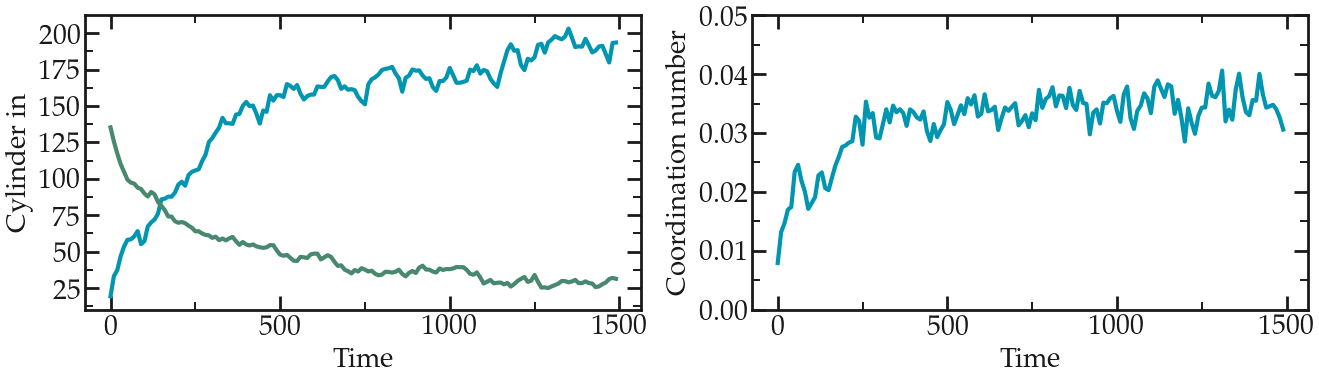
\includegraphics[width=\linewidth]{tutorials/level0/lennard-jones-fluid/population-light.png}
\end{figure}

\section{What now?}

\noindent Now that you have completed this simple molecular dynamics tutorials, what can you do?

\subsection{Play around}

\noindent A good way to progress with LAMMPS and molecular dynamics
simulations is to play around with a script that is already
working and observe the differences and/or errors occurring:
Try adding new commands (you can choose from the documentation),
try removing some of the commands, try changing the parameter values
(see also the first exercise below).
The more you trigger warnings, the easier it will be for you to solve your
own simulation.

\subsection{Try another tutorial}

\noindent There are many common aspects of molecular simulations that were not dealt with in this
tutorial:
\begin{itemize}
\item dealing with charged atoms and bounded molecules, as is necessary to model most existing molecules, solids, or structures, see for instance :ref:`all-atoms-label` and :ref:`sheared-confined-label`,
\item dealing with non-constant volume,
\item dealing with reactivity and bond formation/breaking, see :ref:`reactive-silicon-dioxide-label`.
\end{itemize}

\section{Exercises}

\noindent \subsection{A simulation with no thermostat}

So far, simulations were made using the NVT ensemble [constant number 
of atoms, N, constant volume V, and constant (or at least imposed)
temperature T].
Run a similar simulation in the NVE ensemble, and extract the
total energy of the system over time.

\begin{tcolorbox}[colback=mylightblue!5!white,colframe=mylightblue!75!black,title=Expected output]
Make sure that the total energy is conserved over time, as see here. Note also 
that the kinetic energy constantly exchanges with the potential energy.
\end{tcolorbox}

\noindent \subsection{Do without the *minimize* command}

Run a successful simulation without using the \textit{minimize} command.
The absence of energy minimization needs to be compensated
in order to avoid triggering the \textit{ERROR: Lost atoms} message.

\begin{tcolorbox}[colback=mylightblue!5!white,colframe=mylightblue!75!black,title=Hints]
The value of the timestep and/or the damping factor of the fix langevin
can be tuned to prevent the system from exploding.
Perform as many consecutive runs with varying timestep and damping
factors that you feel are necessary.
Have a look at fix nve/limit. This command was
made to prevent an unequilibrated system from exploding
by preventing atoms to travel too far every timestep.
\end{tcolorbox}

\noindent \subsection{Non-equilibrium simulation}

So far, atoms were freely diffusing without contraint or external force.
Add an external force to induce a net flow of atoms in one
direction. The magnitude of the force must be chosen so
that the system is not \textit{too far} from equilibrium.

\begin{tcolorbox}[colback=mylightblue!5!white,colframe=mylightblue!75!black,title=Hints]
LAMMPS offers several option to add external force to a system, one 
being the fix addforce.
Note: If the system is too far from equilibrium, it enters the non-linear response 
regimes and its properties and parameters will differ from its equilibrium values.
In general, this is something that you must avoid (unless you are studying
non-linear effects). 
\end{tcolorbox}

\noindent \subsection{Dumbbell molecules}

Add a bond between couple of identical atoms to create
dumbbell molecules, just like in the image:

\begin{figure}
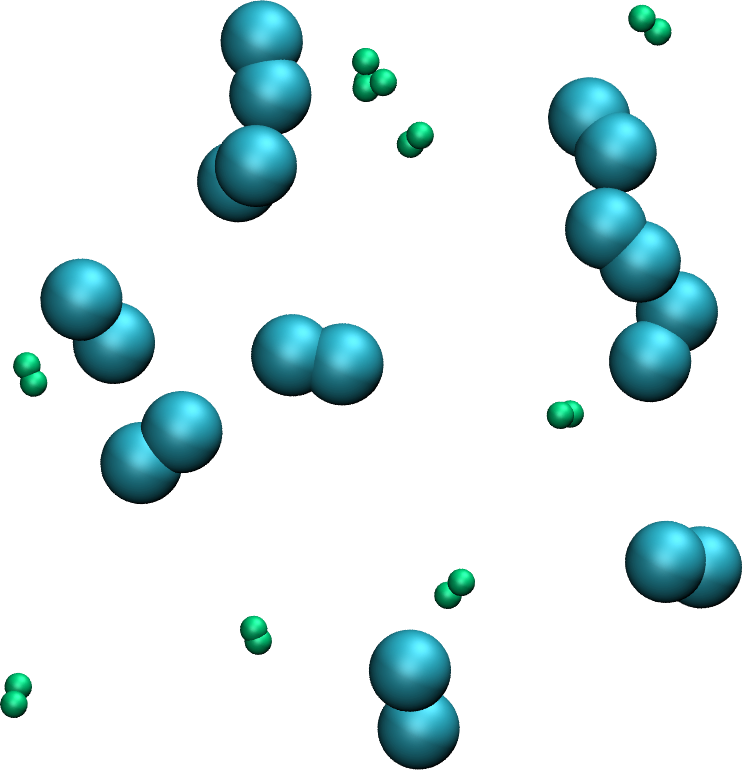
\includegraphics[width=\linewidth]{tutorials/level0/lennard-jones-fluid/dumbell-light.png}
\end{figure}

\begin{tcolorbox}[colback=mylightblue!5!white,colframe=mylightblue!75!black,title=Hints]
Use molecule template to easily insert as many atoms connected
by bonds (i.e. molecules) as you want. A molecule 
template typically begins as follow:
\begin{lcverbatim}
# Dumbell molecule
2 atoms
1 bonds
Coords
1 0.5 0 0
2 -0.5 0 0
(...)
\end{lcverbatim}

\noindent \end{tcolorbox}


\chapter{Breaking a carbon nanotube}

\vspace{-1cm} \noindent \textcolor{graytitle}{\textit{{\Large Breaking the bonds of a carbon nanotube under deformation}}\vspace{0.5cm} }

\noindent \hspace{-0.45cm}\begin{wrapfigure}{r}{4cm}
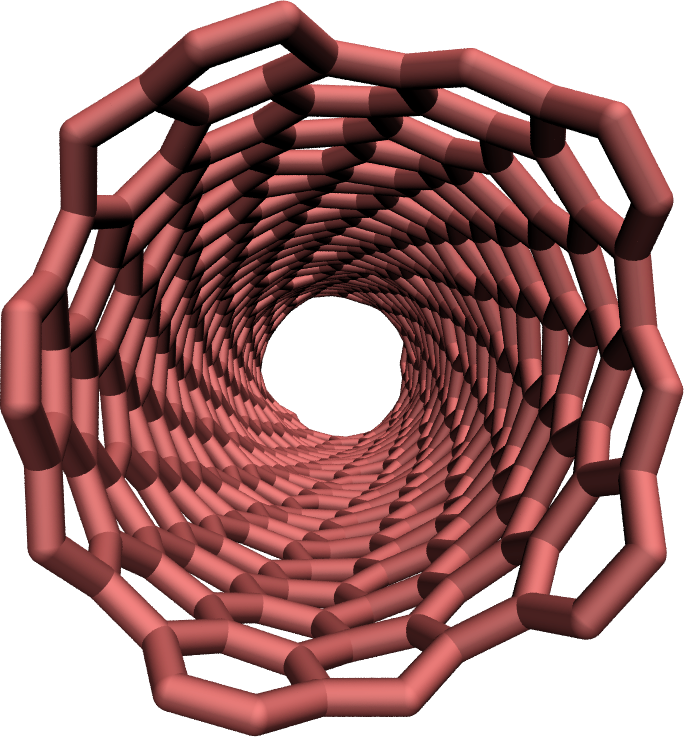
\includegraphics[width=4cm]{tutorials/level1/breaking-a-carbon-nanotube/CNT_light.png}
\end{wrapfigure}

\noindent In this tutorial, two force fields, a classic one and a reactive one (airebo) 
are used to simulate the deformation of a carbon nanotube (CNT). With the reactive 
force field, the breaking of the $C-C$ bonds during the plastic deformation of the CNT is 
simulated.

\section{Unbreakable bonds}

\noindent A CNT with unbreakable bonds is generated and exposed to deformations.

\subsection{System creation}

\noindent The initial configuration (atoms positions, bonds, angles,
etc.) is generated using \href{https://www.ks.uiuc.edu/Research/vmd/}{VMD}. Open VMD,
and go to Extensions, Modeling, Nanotube Builder. A window
named Carbon Nanostructures opens up, allowing us to choose
between generating sheet or nanotube of graphene or BN. For
this tutorial, let us generate a carbon nanotube.
Keep all default values, and click on "Generate
Nanotube". You should something like the image on the top right 
of this page.
At this point, this is not a molecular dynamics simulation,
but a cloud of unconnected dots. In the VMD terminal, set the
box dimensions by typing the following commands in the VMD terminal:

\begin{lcverbatim}
molinfo top set a 80  
molinfo top set b 80            
molinfo top set c 80 
\end{lcverbatim}

\noindent The values of 80 in each direction have been chosen
so that the box is much larger than the carbon nanotube.
In order to generate the initial LAMMPS data file, let us use Topotool:
to generate the LAMMPS data file, enter the following command:

\begin{lcverbatim}
topo writelammpsdata cnt_molecular.data molecular
\end{lcverbatim}

\noindent Here molecular refers to the LAMMPS \textit{atom$\_$style}, and
\textit{cnt$\_$molecular.data} to the name of the file. 

\begin{tcolorbox}[colback=mylightblue!5!white,colframe=mylightblue!75!black,title=About TopoTools]
Note that I am using TopoTools v1.7. Older or newer versions 
may require slightly different commands. 
More details about these commands can be found on the
personal page of \href{https://sites.google.com/site/akohlmey/software/topotools}{Axel Kohlmeyer}.
In short, Topotools deduces the location of bonds, angles,
dihedrals, and impropers from the positions of the atoms,
and generates a file that can be read by LAMMPS.
\end{tcolorbox}

\noindent The parameters of the constraints (bond length,
dihedral coefficients, etc.) will be given later.
A new file named \textit{cnt$\_$molecular.data} has been created, it starts
like that:

\begin{lcverbatim}
LAMMPS data file. CGCMM style. atom_style molecular generated by VMD/TopoTools v1.7 on Fri Aug 04 11:29:35 CEST 2023
700 atoms
1035 bonds
2040 angles
4030 dihedrals
670 impropers
1 atom types
1 bond types
1 angle types
1 dihedral types
1 improper types
-40.000000 40.000000  xlo xhi
-40.000000 40.000000  ylo yhi
-12.130411 67.869589  zlo zhi

(...)
\end{lcverbatim}

\noindent The \textit{cnt$\_$molecular.data} file contains information
about the positions of the carbons atoms, as well as the
identity of the atoms that are linked by bonds, angles, dihedrals,
and impropers constraints.
Save the \textit{cnt$\_$molecular.data} file in the same folder as your
future LAMMPS input script.
We are done with the system
generation, we can start the molecular dynamics simulations.
Alternatively, you can download the file I did generate 
by clicking  \href{../../../../../inputs/level1/breaking-a-carbon-nanotube/unbreakable-bonds/cnt_molecular.data}{here}, and continue with the tutorial.

\subsection{Generic options}

\noindent Create a new text file and name it "input.lammps". Copy the
following lines in it:

\begin{lcverbatim}
# Initialisation
variable T equal 300
units real
atom_style molecular
boundary f f f
pair_style lj/cut 14
bond_style harmonic
angle_style harmonic
dihedral_style opls
improper_style harmonic
special_bonds lj 0.0 0.0 0.5
read_data cnt_molecular.data
\end{lcverbatim}

\noindent The chosen unit system is real (distances are in Angstrom, time in femtosecond),
atom style is molecular (atoms are dots that can be bonded with each other),
and the boundary conditions are fixed. The boundary conditions
do not matter much here, as the box boundaries are far from the graphene sheet. 
Here the pair style is lj/cut (i.e. a Lennard Jones potential 
with a short range cutoff) with
parameter 14, which means that the atoms closer than 14
Angstroms from each others interact through a Lennard-Jones
potential. Notice that there is no Coulombic interaction
because there are no partial charges.
The bond, angle, dihedral, and improper styles specify the
different potentials used to restrain the positions of the
atoms. For more details, have a look at the LAMMPS website
(see for example the page of the \href{https://lammps.sandia.gov/doc/dihedral_opls.html}{OPLS dihedral style}).

The last command (\textit{read$\_$data}) imports the carbon.data file
previously generated with VMD, which contains the
information about the box size, atoms positions, etc.

\begin{tcolorbox}[colback=mylightblue!5!white,colframe=mylightblue!75!black,title=About interaction between neighbors atoms]
Atoms connected by a bond do not typically interact through
Lennard-Jones interaction. This is ensured here by the
\textit{special$\_$bonds} command. The three numbers of the
\textit{special$\_$bonds} command are weighting factors for the
Lennard-Jones interaction between atoms connected by bond
(respectively directly bounded $C-C$, separated by two bonds $C-C-C$,
and separated by three bonds $C-C-C-C$). For instance, the
first weighting factor, with a
value of 0, imposes that two atoms connected by a bond do
not interact through a Lennard-Jones potential (therefore
they only interact through the harmonic potential that bond the atoms
of the graphene).
\end{tcolorbox}

\noindent \subsection{Parameters}

We need to specify the parameters of both bonded and
non-bonded functions. Create a new text file in the same
folder and name it "parm.lammps". Copy the following lines
in it:

\begin{lcverbatim}
pair_coeff 1 1 0.066047 3.4
bond_coeff 1 469 1.4
angle_coeff 1 63 120
dihedral_coeff 1 0 7.25 0 0
improper_coeff 1 5 180
\end{lcverbatim}

\noindent The \textit{pair$\_$coeff} command sets the Lennard-jones parameters
$\epsilon$ and $\sigma$ for the only type of
atom of the simulation: carbon atom of type 1. The
\textit{bond$\_$coeff} provides the equilibrium distance $r_0$ as
well as the spring constant $K$ for the harmonic
potential imposed between two neighboring carbon atoms,
where the potential is $E = K_r ( r - r_0)^2$. The
\textit{angle$\_$coeff} gives the equilibrium angle $theta_0$ and
constant for the potential between three neighbors atoms :
$E = K_\theta ( \theta - \theta_0)^2$. The \textit{dihedral$\_$coeff}
and \textit{improper$\_$coeff} give the potential for the constraints
between 4 atoms. The file PARM.lammps need to be included in the
simulation by adding the following line to input.lammps:

\begin{lcverbatim}
include parm.lammps
\end{lcverbatim}

\noindent \subsection{Prepare initial state}

Depending on VMD and topotool version, the CNT may or may not be centered in 
the box. Let us make sure that we start from a clean initial state by
recentering the CNT at the origin (0, 0, 0). In addition, the box boundaries 
are not symmetric with respect to (0, 0, 0), as seen in \textit{cnt$\_$molecular.data}:

\begin{lcverbatim}
-40.000000 40.000000  xlo xhi
-40.000000 40.000000  ylo yhi
-12.130411 67.869589  zlo zhi

\end{lcverbatim}

\noindent Let us recenter the CNT:

\begin{lcverbatim}
group carbon_atoms type 1
variable carbon_xcm equal -1*xcm(carbon_atoms,x)
variable carbon_ycm equal -1*xcm(carbon_atoms,y)
variable carbon_zcm equal -1*xcm(carbon_atoms,z)
displace_atoms carbon_atoms move ${carbon_xcm} ${carbon_ycm} ${carbon_zcm}
\end{lcverbatim}

\noindent The first command includes all of the atoms of type one
(i.e. all the atoms here) in a group named \textit{carbon$\_$atoms}. 
The 3 variables measure the current position of the group \textit{carbon$\_$atoms}
along all 3 directions, respectively. Then, the displace atoms 
command move the group \textit{carbon$\_$atoms}, ensuring that its center of mass 
is located at the origin (0, 0, 0).
Let us also change the box boundaries:

\begin{lcverbatim}
change_box all x final -40 40 y final -40 40 z final -40 40
\end{lcverbatim}

\noindent \begin{tcolorbox}[colback=mylightblue!5!white,colframe=mylightblue!75!black,title=Note]
Such cleaner and more symmetrical initial state can simplify
future data analysis.
\end{tcolorbox}

\noindent In order to impose a force to the edges of the CNT, let us isolate the
atoms from the two edges of the CNT and place them into different groups.
Later, the displacement will be applied to the atoms of the edges.
Add the following lines to the input script:

\begin{lcverbatim}
variable zmax equal bound(carbon_atoms,zmax)-0.5
variable zmin equal bound(carbon_atoms,zmin)+0.5
region rtop block INF INF INF INF ${zmax} INF
region rbot block INF INF INF INF INF ${zmin}
region rmid block INF INF INF INF ${zmin} ${zmax}
\end{lcverbatim}

\noindent \begin{lcverbatim}
group carbon_top region rtop
group carbon_bot region rbot
group carbon_mid region rmid
\end{lcverbatim}

\noindent The atoms of the edges as selected within the \textit{carbon$\_$top} and \textit{carbon$\_$bot} groups 
are represented with a different color:

\begin{figure}
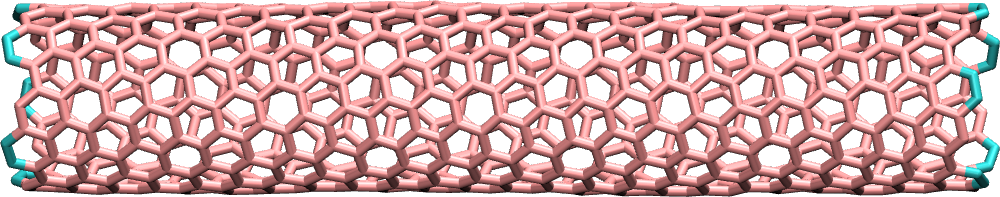
\includegraphics[width=\linewidth]{tutorials/level1/breaking-a-carbon-nanotube/light_colored_edges.png}
\end{figure}

When running a simulation, the number of atoms in each
group is printed in the terminal (and in the log.lammps
file). Always make sure that the number of atoms in each group 
is reasonable, just like here:

\begin{lcverbatim}
10 atoms in group carbon_top
10 atoms in group carbon_bot
680 atoms in group carbon_mid
\end{lcverbatim}

\noindent \subsection{Thermalisation and dynamics}

Let us specify the thermalisation and the dynamics of the
system. Add the following lines to \textit{input.lammps}:

\begin{lcverbatim}
velocity carbon_mid create ${T} 48455 mom yes rot yes
fix mynve all nve
compute Tmid carbon_mid temp
fix myber carbon_mid temp/berendsen ${T} ${T} 100
fix_modify myber temp Tmid
\end{lcverbatim}

\noindent The \textit{velocity$\_$create} command gives initial velocities to
the atoms of the middle group \textit{carbon$\_$mid}, ensuring an initial temperature
of 300 K for these atoms with no overall translational momentum (\textit{mom yes})
nor rotational momentum (\textit{rot yes}).
The \textit{fix nve} is applied to all atoms so that all atom positions are recalculated
every timestep. 

A Berendsen thermostat is applied to the atoms
of the group \textit{carbon$\_$mid} only. The \textit{fix$\_$modify myber} ensures that the
fix Berendsen uses the temperature of the group \textit{carbon$\_$mid} as an
input, instead of the temperature of whole system. This is necessary
to make sure that the frozen edges won't bias the temperature. Note that the atoms
of the edges do not need a thermostat because their motion will
be restrained, see below.

\begin{tcolorbox}[colback=mylightblue!5!white,colframe=mylightblue!75!black,title=Deal with semi-frozen system]
Always be careful when part of a system is frozen. In that 
case, the total temperature of the system is effectively lower
than the applied temperature because the frozen atoms 
have no thermal motion. If you have any doubt about the procedure
you are using, simply check the temperature of the non-frozen group, for
example using the fix ave/time:
\begin{lcverbatim}
fix at1 all ave/time 10 100 1000 c_Tmid file temperature_middle_group.dat
\end{lcverbatim}

\noindent \end{tcolorbox}

\subsection{Deal with frozen edges}

\noindent To restrain the motion of the atoms at the edges, let us add the
following commands:

\begin{lcverbatim}
\end{lcverbatim}

\noindent The two \textit{setforce} commands cancel the forces applied on the
atoms of the two edges, respectively. A fix setforce applies at every step of the
simulation, and are here applying along all 3 directions: $x$, $y$
and $z$. The two velocity commands set the initial velocities along $x$,
$y$, and $z$ to 0 for the atoms of the edges. 

As a consequence of these last four commands, the atoms of the edges will remain
immobile during the simulation (or at least they would if no other command was
applied to them).

\begin{tcolorbox}[colback=mylightblue!5!white,colframe=mylightblue!75!black,title=On imposing a constant velocity to a system]
The \textit{velocity set} commands impose the velocity of a group of atoms when it is 
read, but do not enforce the velocity during the entire simulation. 
When \textit{velocity set} is used in combination with \textit{setforce 0 0 0}, the atoms
wont feel any force during the entire simulation. According to the Newton equation,
no force means no acceleration, meaning that the initial velocity will persist.
\end{tcolorbox}

\noindent \subsection{Data extraction}

Next, in order to measure the strain and stress suffered by the
CNT, let us extract the distance $L$ between
the two edges as well as the force applied on the edges.

\begin{lcverbatim}
variable L equal xcm(carbon_top,z)-xcm(carbon_bot,z)
fix at2 all ave/time 10 100 1000 v_L file length.dat
fix at3 all ave/time 10 100 1000 f_mysf1[3] f_mysf2[3] file force.dat
\end{lcverbatim}

\noindent Let us also add a command to print the atom coordinates in a
lammpstrj file every 1000 steps.

\begin{lcverbatim}
dump mydmp all atom 1000 dump.lammpstrj
\end{lcverbatim}

\noindent \begin{tcolorbox}[colback=mylightblue!5!white,colframe=mylightblue!75!black,title=About extracting quantity from variable compute or fix]
Notice that the values of the force on each edge are
extracted from the fixes setforce \textit{mysf1} and \textit{mysf2}, simply by
calling them using \textit{f$\_$}, the same way variables are called
using \textit{v$\_$} and computes are called using \textit{c$\_$}. A fix
setforce cancels all the forces on a group of atoms at every
step, but allows one to extract the values of the force
before its cancellation.
\end{tcolorbox}

\noindent \subsection{Molecular dynamics run}

Let us run a small equilibration step to bring the system 
to the required temperature without applying any deformation:

\begin{lcverbatim}
thermo 100
thermo_modify temp Tmid
timestep 1.0
run 5000
\end{lcverbatim}

\noindent With the \textit{thermo$\_$modify} command, we specify to LAMMPS that we
want the temperature $T_\mathrm{mid}$ to be printed in
the terminal, not the temperature of the entire system
(because of the frozen edges, the temperature of the entire
system is not relevant). 

\subsection{Option A: Incremental deformation}

\noindent A first possibility to deform the CNT is to 
use the loop function of LAMMPS. 
Let us perform a loop (indentation is optional):

\begin{lcverbatim}
variable var loop 50
\end{lcverbatim}

\noindent At each step of the loop, the edges are slightly displaced, and
the simulation runs for 1000. Then the variable \textit{var} is iterated
by the \textit{next var}, and the simulation \textit{jumps} back to the beginning of 
the loop. It will be repeated 50 times, for a total elongation
equal to $2 \times 0.1 \times 50 = 10$ Angstroms. Increase the number of iteration 
for larger deformation.
You should observe the CNT being progressively elongated
and being deformed.
With the present force field, no matter how large is the
imposed deformation, the bonds will never break. To study
such bond breaking, one has to use a reactive force
field, which is done in some other tutorials here (like :ref:`carbon-nanotube-label`).

\subsection{Option B: Constant-velocity}

\noindent To ensure a smooth step-less deformation of the sheet,
let us impose a constant velocity deformaiton by combining
the "velocity set" command with the "fix setforce". 
To obtain the same elongation as previously (i.e. 5 Angstrom 
per edge) when using a velocity for each edge of 0.0005 Angstroms per
femtosecond (or 50 meters per second), the simulation 
must last 5 / 0.0005 = 10000 femtoseconds. 
Remove the previous loop and replace it with:

\begin{lcverbatim}
velocity carbon_top set NULL NULL 0.0005
velocity carbon_bot set NULL NULL -0.0005
run 10000
\end{lcverbatim}

\noindent \section{Breakable bonds}

Let us do the same type of simulation, but using a reactive force field 
instead, allowing for the bonds to break.

\subsection{Input file}

\noindent In a different folder, create a LAMMPS input file, call it
input.lammps, and type in it:

\begin{lcverbatim}
# Initialisation
variable T equal 300
units metal
atom_style molecular
boundary p p p
pair_style airebo 2.5 1 1
\end{lcverbatim}

\noindent A difference with the previous part
is the unit system, here 'metal' instead of 'real', a choice
that is imposed by the airebo force field.

\begin{tcolorbox}[colback=mylightblue!5!white,colframe=mylightblue!75!black,title=About metal units]
With metal units, the time is in pico second, 
distances are in Angstrom, and the energy is in eV.
\end{tcolorbox}

\noindent Let us prepare the data file. Duplicate the 
previous file \textit{cnt$\_$molecular.data}, name the copy \textit{cnt$\_$atom.data},
place it within the 
current folder, and remove all bond, angle, and dihedral 
information so that \textit{cnt$\_$atom.data} look like that: 

\begin{lcverbatim}
700 atoms
1 atom types
-40.000000 40.000000  xlo xhi
-40.000000 40.000000  ylo yhi
-12.130411 67.869589  zlo zhi
Masses
1 12.010700 # CA
Atoms # molecular
1 1 1 5.162323 0.464617 8.843235 # CA CNT
2 2 1 4.852682 1.821242 9.111212 # CA CNT
(...)
\end{lcverbatim}

\noindent Remove also everything that comes after for \textit{Bonds}
keyword, so that the last lines of the file look like that:

\begin{lcverbatim}
(...)
697 697 1 4.669892 -2.248901 45.824036 # CA CNT
698 698 1 5.099893 -0.925494 46.092010 # CA CNT
699 699 1 5.162323 -0.464617 47.431896 # CA CNT
700 700 1 5.099893 0.925494 47.699871 # CA CNT
\end{lcverbatim}

\noindent The reason the bond information is not needed here is that 
a reactive force field is used. Such force field 
deduces the bonds between atoms on the fly based on the positions of the atoms.
When two initially bonded atoms are separated by a 
distance that is too large, the bond may break. 
You can also download the file I did generate 
by clicking \href{../../../../../inputs/level1/breaking-a-carbon-nanotube/breakable-bonds/cnt_atom.data}{here}.

Then, let us import the LAMMPS data file, and set the
pair coefficients:

\begin{lcverbatim}
# System definition
read_data cnt_atom.data
pair_coeff * * CH.airebo C
\end{lcverbatim}

\noindent Here, there is one single atom type. We impose this type
to be carbon by using the the letter C.
The CH.airebo file can be downloaded \href{../../../../../inputs/level1/breaking-a-carbon-nanotube/breakable-bonds/CH.airebo}{here}.
The rest of the script is very similar to the previous one:

\begin{lcverbatim}
change_box all x final -40 40 y final -40 40 z final -60 60
group carbon_atoms type 1
variable carbon_xcm equal -1*xcm(carbon_atoms,x)
variable carbon_ycm equal -1*xcm(carbon_atoms,y)
variable carbon_zcm equal -1*xcm(carbon_atoms,z)
displace_atoms carbon_atoms move ${carbon_xcm} ${carbon_ycm} ${carbon_zcm}
variable zmax equal bound(carbon_atoms,zmax)-0.5
variable zmin equal bound(carbon_atoms,zmin)+0.5
region rtop block INF INF INF INF ${zmax} INF
region rbot block INF INF INF INF INF ${zmin}
region rmid block INF INF INF INF ${zmin} ${zmax}
group carbon_top region rtop
group carbon_bot region rbot
group carbon_mid region rmid
velocity carbon_mid create ${T} 48455 mom yes rot yes
fix mynve all nve
compute Tmid carbon_mid temp
fix myber carbon_mid temp/berendsen ${T} ${T} 0.1
fix_modify myber temp Tmid
\end{lcverbatim}

\noindent Note that a larger distance was used for the box size along 
the z axis, to allow for larger deformation. The \textit{change$\_$box}
was placed before the \textit{displace$\_$atoms} to avoid issue with the 
CNT crossing the edge of the box.
Let us impose a constant velocity deformation using the atoms
of one edge, while maintaining the other edge fix. Do to so,
one needs to cancel the forces (thus the acceleration) on
the atoms of the edges using the setforce command, and set
the value of the velocity along the z direction.

\subsection{Equilibration}

\noindent First, as an equilibration step, let us set the velocity to 0
for the atoms of the edge. Let us fully constraint the bottom edge, 
and constraint the top edge only along z.

\begin{lcverbatim}
fix mysf1 carbon_bot setforce 0 0 0
fix mysf2 carbon_top setforce NULL NULL 0
velocity carbon_bot set 0 0 0
velocity carbon_top set NULL NULL 0
variable pos equal xcm(carbon_top,z)
fix at1 all ave/time 10 100 1000 v_pos file cnt_deflection.dat
fix at2 all ave/time 10 100 1000 f_mysf1[3] f_mysf2[3] file edge_force.dat
dump mydmp all atom 1000 dump.lammpstrj
thermo 100
thermo_modify temp Tmid
timestep 0.0005
run 5000
\end{lcverbatim}

\noindent At the start of the equilibration, you can see that the
temperature deviates from the target temperature of 300 K, but
after a few picoseconds it reaches the target value:

\begin{lcverbatim}
Step          Temp          E_pair         E_mol          TotEng         Press     
0   300           -5084.7276      0             -5058.3973     -1515.7017    
100   237.49462     -5075.4114      0             -5054.5671     -155.05545    
200   238.86589     -5071.9168      0             -5050.9521     -498.15029    
300   220.04074     -5067.1113      0             -5047.7989     -1514.8516    
400   269.23434     -5069.6565      0             -5046.0264     -174.31158    
500   274.92241     -5068.5989      0             -5044.4696     -381.28758    
600   261.91841     -5065.985       0             -5042.9971     -1507.5577    
700   288.47709     -5067.7301      0             -5042.4111     -312.16669    
800   289.85177     -5066.5482      0             -5041.1086     -259.84893    
900   279.34891     -5065.0216      0             -5040.5038     -1390.8508    
1000   312.27343     -5067.6245      0             -5040.217      -465.74352
(...)
\end{lcverbatim}

\noindent \subsection{Deformation}

After equilibration, let us set the velocity to 30 m/s and run for
a longer time:

\begin{lcverbatim}
# 0.15 A/ps = 30 m/s
velocity carbon_top set NULL NULL 0.15
run 280000
\end{lcverbatim}

\noindent The CNT should break around the step 250000. If not, either 
run for a longer time or for a slightly larger velocity.
When looking at the lammpstrj file using VMD, you will see
the bonds breaking, similar to \href{https://www.youtube.com/watch?v=f1ve1j3yA6w}{this video}. Use
the DynamicBonds representation.

\hspace{-0.45cm}\begin{wrapfigure}{r}{4cm}
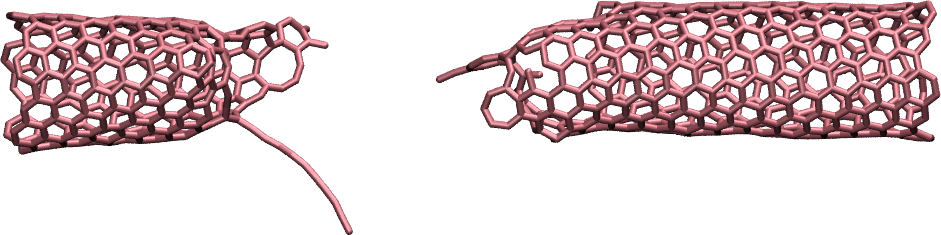
\includegraphics[width=4cm]{tutorials/level1/breaking-a-carbon-nanotube/deformed-light.png}
\end{wrapfigure}

\noindent Figure : Carbon nanotube after being broken.

\begin{tcolorbox}[colback=mylightblue!5!white,colframe=mylightblue!75!black,title=About bonds in VMD]
Note that VMD guesses bonds based on the distances
between atoms, and not based on the presence of actual
bonds between atoms in the LAMMPS simulation. Therefore what is seen
in VMD can sometimes be misleading.
\end{tcolorbox}

\noindent \subsection{Post-mortem analysis (Python)}

There are two main ways to analyse data from a MD simulation:
(1) on-the-fly analysis, like what we did with the two fix ave/time,
and (2) post-mortem analysis. Post-mortem analysis can be performed using
the atom coordinate saved in the lammpstrj file.
Here, let us use the open source Python library MDAnalysis.
Open a new Jupyter notebook within the same folder, call it
\textit{bond$\_$evolution.ipynb}. First, let us import libraries
by copying into \textit{bond$\_$evolution.ipynb}:

\begin{lcverbatim}
import MDAnalysis as mda
import numpy as np
\end{lcverbatim}

\noindent Then, let us create a MDAnalysis universe using the LAMMPS
data file (for the topology information) and the dump file 
(for the coordinate evolution over time). Let us detect the
original bonds using the bond guesser of MDAnalysis. Let us also create 
a single atom group containing all the carbon atoms: 

\begin{lcverbatim}
# create a universe from the dump file
# guess bond based on distance from the initial topology
u = mda.Universe("cnt_atom.data", "dump.lammpstrj",
# create a group
cnt = u.select_atoms("type 1")
\end{lcverbatim}

\noindent Note : The bond guesser of MDAnalysis will not update the list of bond
over time, so we will need to use a few trick.
Then, let us loop over the trajectory and extract bond length and number
over time:

\begin{lcverbatim}
nbond_vs_time = []
lbond_vs_time = []
# loop over trajectory
for ts in u.trajectory:
nbond_vs_time = np.array(nbond_vs_time)
lbond_vs_time = np.array(lbond_vs_time)
\end{lcverbatim}

\noindent The array \textit{nbond$\_$vs$\_$time} contains the number of bond as a function of time, and 
\textit{lbond$\_$vs$\_$time} the bond length. Let us plot both of them:

\begin{figure}
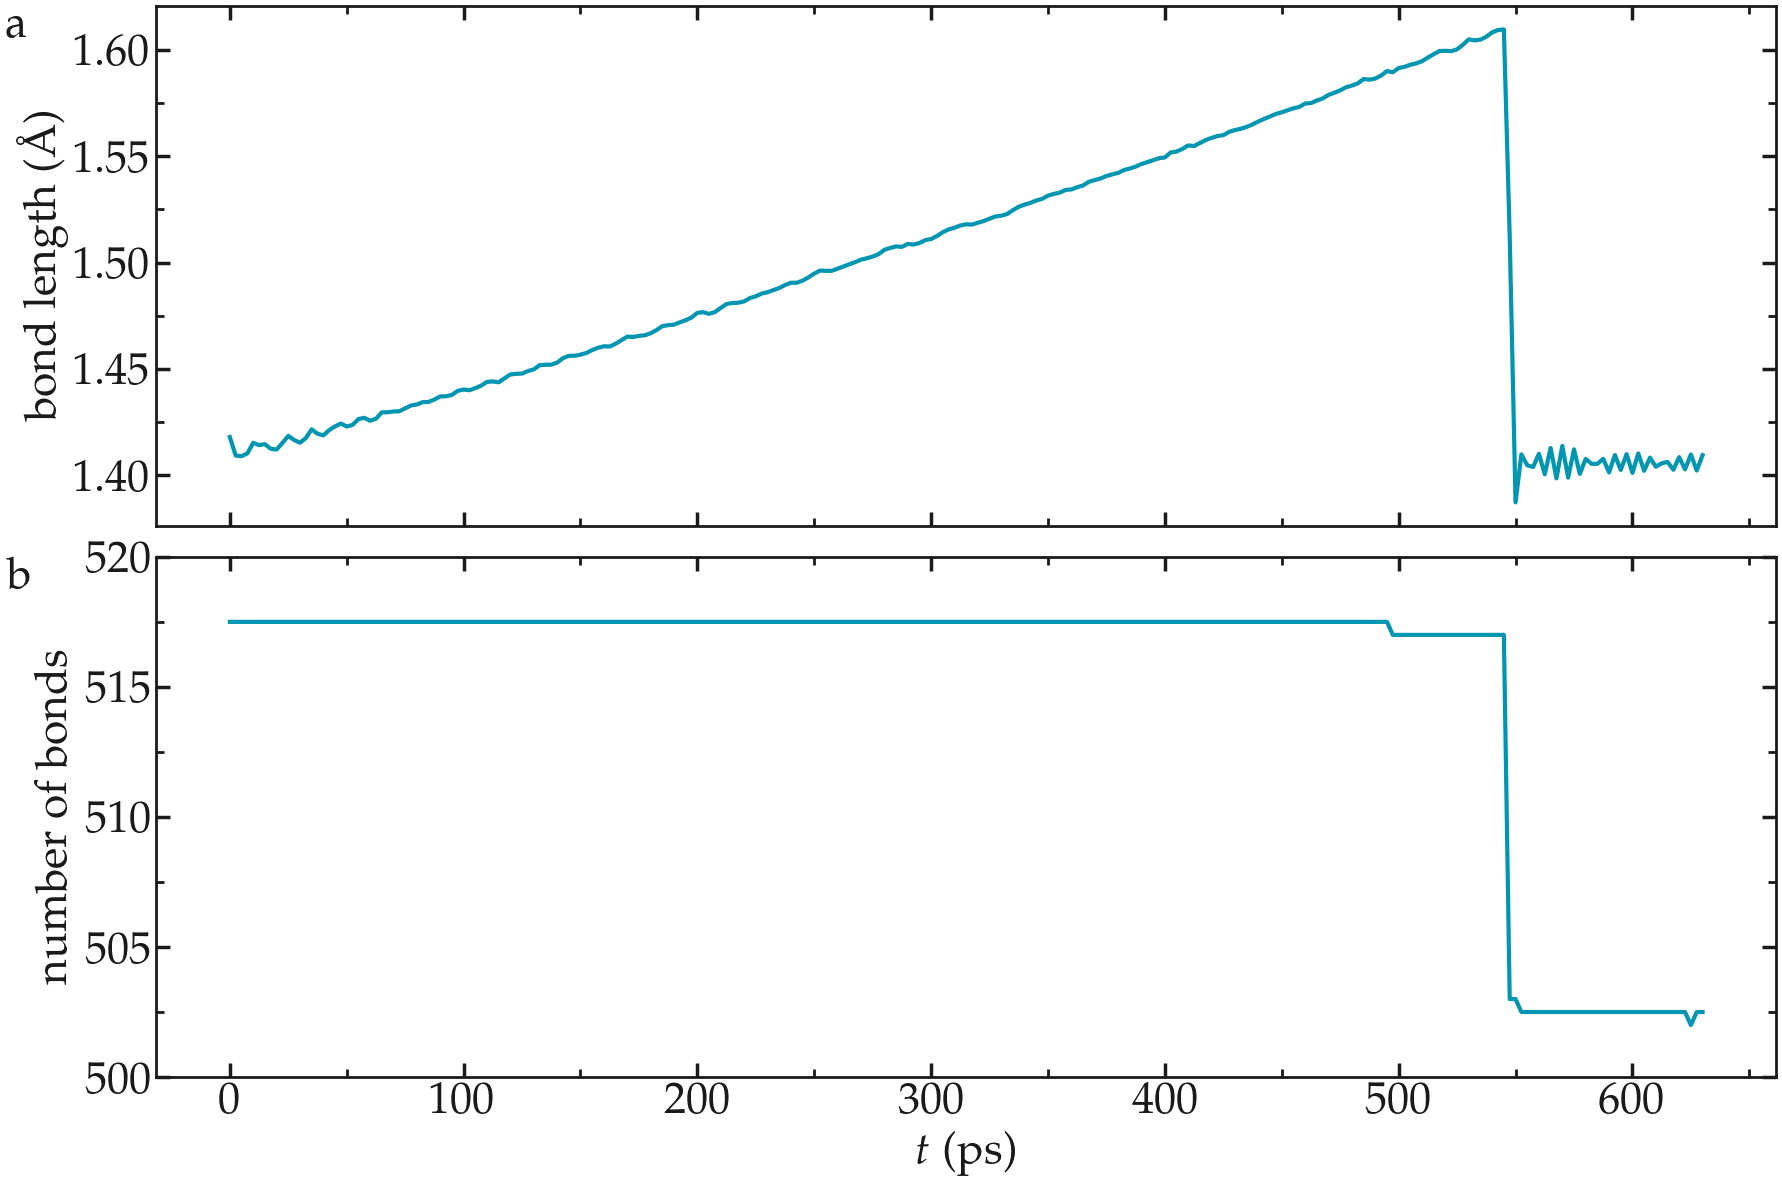
\includegraphics[width=\linewidth]{tutorials/level1/breaking-a-carbon-nanotube/bond-light.png}
\end{figure}

\section{Going further with exercises}

\noindent \subsection{Isolated nanotube}

When a rubber band is streched up, it heats up due to entropy change. 
In the current simulation, the constant exchange of energy with the 
thermostat prevents the temperature to evolve significantly, even under
strong deformation.
Remove the thermostat and observe the evolution of the temperature of an
\textit{isolated} carbon nanotube being deformed. Does it heat-up? Or does it cool down?

\hspace{-0.45cm}\begin{wrapfigure}{r}{4cm}
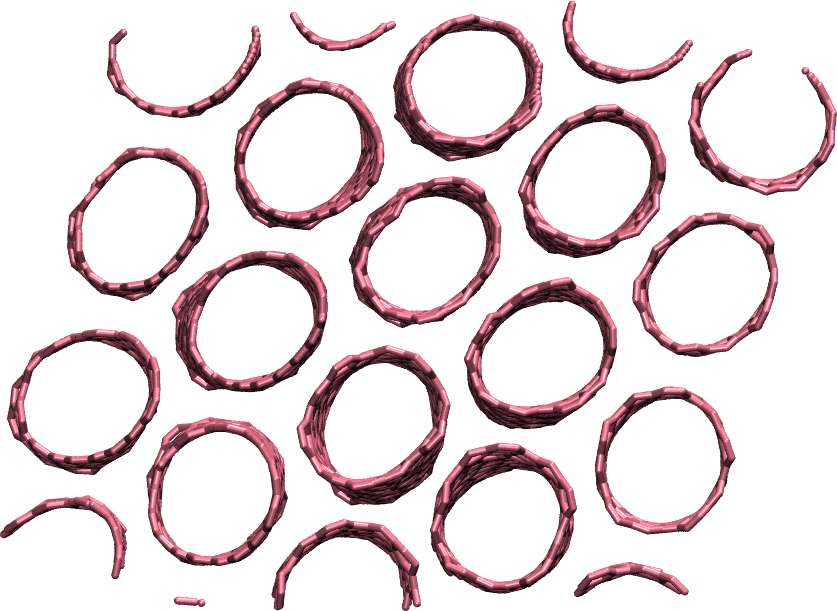
\includegraphics[width=4cm]{tutorials/level1/breaking-a-carbon-nanotube/shared-light.png}
\end{wrapfigure}

\noindent \subsection{Deforming membrane}

Replicate the CNT along x and y, and equilibrate the system to 
create a membrane, just like the image on the right. 
Then, apply a shear deformation along xy.

\begin{tcolorbox}[colback=mylightblue!5!white,colframe=mylightblue!75!black,title=Hints (click to reveal)]
The box must be converted to triclinic to support deformation
along xy.
\end{tcolorbox}

\noindent \hspace{-0.45cm}\begin{wrapfigure}{r}{4cm}
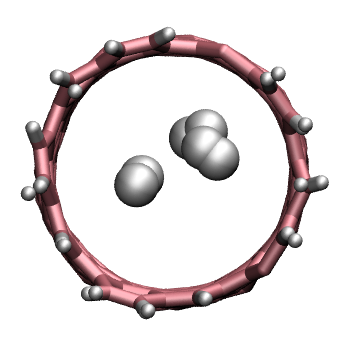
\includegraphics[width=4cm]{tutorials/level1/breaking-a-carbon-nanotube/CH-light.png}
\end{wrapfigure}

\noindent \subsection{Decorate the CNT}

Add hydrogen atoms randomly to the system (using the same
airebo force field). 
Equilibrate the system. After some time, some hydrogen atoms will 
decorate the free carbon atoms at the edge of the CNT. Some 
other hydrogen atoms will bond and form H2 molecules. 

\subsection{Strain-stress curve}

\noindent Adapt the current script and extract a full strain-stress curve.

\begin{figure}
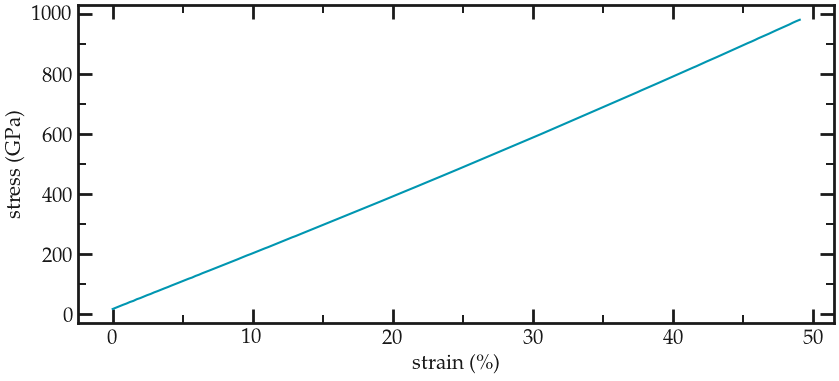
\includegraphics[width=\linewidth]{tutorials/level1/breaking-a-carbon-nanotube/strain-stain-curve-light.png}
\end{figure}

\begin{tcolorbox}[colback=mylightblue!5!white,colframe=mylightblue!75!black,title=Hints]
The following steps are optional, but give a better result:
\begin{itemize}
\item only record data during the production run, not the equilibration
\item reduce the velocity to perform a nice and slow pulling of the graphene sheet
\item increase the magnitude of the total elongation
\end{itemize}
\end{tcolorbox}


\chapter{Polymer in water}
\label{all-atoms-label}

\vspace{-1cm} \noindent \textcolor{graytitle}{\textit{{\Large Stretching a small solvated molecule}}\vspace{0.5cm} }

\noindent \hspace{-0.45cm}\begin{wrapfigure}{r}{4cm}
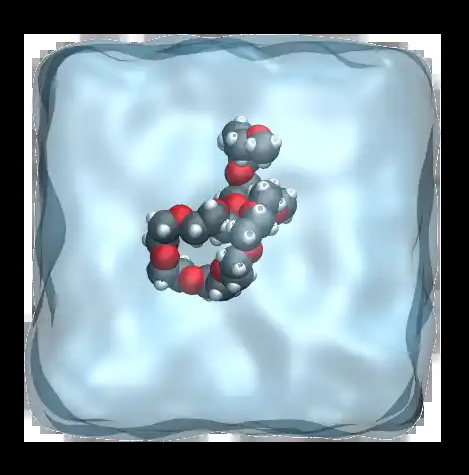
\includegraphics[width=4cm]{tutorials/level2/polymer-in-water/video-PEG-light.png}
\end{wrapfigure}

\noindent The goal of this tutorial is to use LAMMPS and
create a small hydrophilic polymer (PEG -
PolyEthylene Glycol) in a reservoir of water. 
An all-atom description is used, therefore all species considered here
are made of charged atoms connected by bonds constraints.
Once the system is created, a constant stretching force will be applied to both
ends of the polymer, and its length will be measured with time.
This tutorial was inspired by a very nice \href{https://doi.org/10.1021/acsnano.6b07071}{publication} by Liese and coworkers, in which
they compare MD simulations with force spectroscopy experiments.

\section{Bulk water}

\noindent As a first step, a rectangular box of water is created and
equilibrated at ambient temperature and ambient pressure (the PEG molecule will be added in the next sections).
Create a folder named pureH2O/. Inside this folder, create
an empty text file named input.lammps. Copy the following
lines in it:

\begin{lcverbatim}
# LAMMPS input script
units real
atom_style full
bond_style harmonic
angle_style charmm
dihedral_style charmm
pair_style lj/cut/tip4p/long 1 2 1 1 0.105 12.0
kspace_style pppm/tip4p 1.0e-4
\end{lcverbatim}

\noindent There are many differences with respect to
the previous tutorial (\ref{lennard-jones-label}), mostly
because here a system with molecules and partial charges is
modeled (instead of neutral particles). With the unit style \textit{real},
masses are in grams per
mole, distances in Ångstroms, time in femtoseconds, energies
in Kcal/mole. With the atom style \textit{full}, each atom is a dot
with a mass and a charge. In addition, each atom can be
linked by bonds, angles, dihedrals and impropers potentials
(for example to form molecules). The \textit{bond$\_$style},
\textit{angle$\_$style}, and \textit{dihedral$\_$style} commands define the
styles of bond angle, and dihedrals used in the simulation,
respectively, and the \textit{harmonic} and \textit{charmm} keywords
impose the type of potential to use.

\begin{tcolorbox}[colback=mylightblue!5!white,colframe=mylightblue!75!black,title=About the use of charmm style]
The future merging of the water with the PEG
has already been anticipated as the \textit{charmm angle$\_$style}
and \textit{dihedral$\_$style} are requirements of the PEG's model.
A rigid water model will be used here, so the bond
and angle styles that are chosen have no consequence on the water model, they will
only matter to the PEG when it is added.
\end{tcolorbox}

\noindent With the \textit{pair$\_$style} named \textit{lj/cut/tip4p/long}, atoms
interact through both a Lennard-Jones (LJ) potential and
through Coulombic interactions. This pair style is specific to
four points water models, and automatically accounts for the
additional massless site. The six numbers are, respectively,
\begin{itemize}
\item  \textit{}1 -\textit{} the atom type for the oxygen O of the tip4p water,
\item  \textit{}2 -\textit{} the atom type for the hydrogen H of the tip4p water,
\item  \textit{}3 -\textit{} the OH bond type,
\item  \textit{}4 -\textit{} the HOH angle type,
\item  \textit{}5 -\textit{} the distance from O atom to the massless charge (here 0.105 Ångstroms is set by the TIP4P/epsilon water model),
\item  \textit{}6 -\textit{} the cutoff (here of 12 Ångstroms).
\end{itemize}

\begin{tcolorbox}[colback=mylightblue!5!white,colframe=mylightblue!75!black,title=About cutoff in molecular dynamics]
The cutoff of 12 Ångstroms applies to both LJ and Coulombic
interactions, but in a different way. For LJ \textit{cut}
interactions, atoms interact with each others only if they
are separated by a distance smaller than the cutoff. For
Coulombic \textit{long}, interaction between atoms closer than
the cutoff are computed directly, and interaction between
atoms outside that cutoff are computed in the reciprocal
space.
\end{tcolorbox}

\noindent Finally the kspace command defines the long-range solver for the (long)
Coulombic interactions. The pppm style refers to
particle-particle particle-mesh.

\begin{tcolorbox}[colback=mylightblue!5!white,colframe=mylightblue!75!black,title=Background Information (optional) -- About PPPM]
The PPPM
method is based on separating the total interaction
between particles into the sum of short-range
interactions, which are computed by direct
particle-particle summation, and long-range interactions,
which are calculated by solving Poisson's equation using
periodic boundary conditions (PBCs). 
\href{https://doi.org/10.1021/jp9518623}{Luty and van Gunsteren}
\end{tcolorbox}

\noindent Then, let us create a 3D simulation box of dimensions $8 x 3 x 3 \text{nm}^3$,
and make space for 7 atom types (1 and 2 for
the water oxygen and hydrogen, respectively, and 3, 4, 5, 6
and 7 for the PEG molecule (see below)), 6 bond types, 9
angle types, and 14 dihedrals types.

\begin{lcverbatim}
region box block -40 40 -15 15 -15 15
create_box 7 box &
bond/types 6 &
angle/types 9 &
dihedral/types 14 &
extra/bond/per/atom 2 &
extra/angle/per/atom 1 &
extra/special/per/atom 2
\end{lcverbatim}

\noindent \begin{tcolorbox}[colback=mylightblue!5!white,colframe=mylightblue!75!black,title=About extra per atom commands]
The \textit{extra/something/per/atom} commands are here for
memory allocation, they ensure that enough space is left for a
certain number of attribute for each atom. We wont worry
about those commands in this tutorial, just keep that in mind if one day you see the following
error message:
\begin{lcverbatim}
ERROR: Molecule topology/atom exceeds system topology/atom (src/molecule.cpp:1767)
\end{lcverbatim}

\noindent \end{tcolorbox}

Let us include a parameter file containing all the
parameters (masses, interaction energies, bond equilibrium
distances, etc):

\begin{lcverbatim}
include ../PARM.lammps
\end{lcverbatim}

\noindent Next to the \textit{pureH2O/} folder, create a blank file called
\textit{PARM.lammps} and copy the following lines in it:

\begin{lcverbatim}
# Mass
mass 1 15.9994 # H2O O
mass 2 1.008 # H2O H
mass 3 12.011 # CC32A
mass 4 15.9994 # OC30A
mass 5 1.008 # HCA2
mass 6 15.9994 # OC311
mass 7 1.008 # HCP1
# Pair Coeff
pair_coeff 1 1 0.18479 3.165 # H2O - TIP4P - epsilon water model
pair_coeff 2 2 0.0 0.0 # H2O H
pair_coeff 3 3 0.056 3.58141 # CC32A
pair_coeff 4 4 0.100 2.93997 # OC30A
pair_coeff 5 5 0.035 2.38761 # HCA2
pair_coeff 6 6 0.192 3.14487 # OC311
pair_coeff 7 7 0.046 0.40001 # HCP1
# Bond coeff
bond_coeff 1 0 0.9572 # H2O O-H
bond_coeff 2 222.35 1.5300
bond_coeff 3 308.79 1.1111
bond_coeff 4 359.76 1.1415
bond_coeff 5 427.715 1.1420
bond_coeff 6 544.635 0.9600
# Angle coeff
angle_coeff 1 0 104.52 0 0 # H2O H-O-H
angle_coeff 2 50.0000 109.0000 0.0000 0.0000
angle_coeff 3 26.5000 110.1000 22.5300 2.179   
angle_coeff 4 45.0000 111.5000 0.0000 0.0000 
angle_coeff 5 13.0258 109.4000 0.0000 0.0000
angle_coeff 6 35.5000 109.0000 5.4000 1.802
angle_coeff 7 55.0000 108.8900 0.0000 0.0000
angle_coeff 8 75.7000 110.1000 0.0000 0.0000
angle_coeff 9 95.0000 109.7000 0.0000 0.0000
# Dihedral coeff
dihedral_coeff 1 0.57 1 0 0
dihedral_coeff 2 0.29 2 0 0
dihedral_coeff 3 0.43 3 0 0
dihedral_coeff 4 0.59 1 180 0
dihedral_coeff 5 1.16 2 0 0 
dihedral_coeff 6 0.12 1 0 0 
dihedral_coeff 7 0.42 2 0 0
dihedral_coeff 8 0.29 3 0 0
dihedral_coeff 9 2.87 1 180 0
dihedral_coeff 10 0.03 2 0 0
dihedral_coeff 11 0.23 3 0 0
dihedral_coeff 12 1.36 1 180 0
dihedral_coeff 13 0.16 2 0 0
dihedral_coeff 14 1.01 3 0 0
\end{lcverbatim}

\noindent If you want to know which column refers to which
parameter, you can refer to the LAMMPS documentation. For
this tutorial, we will just trust that these parameters
are correct and will lead to physically consistent
behavior. Now, let us create water molecules. To do so, let us
define a water molecule using a molecule template called
\textit{H2OTip4p.txt}, and randomly create 700 of those.

\begin{lcverbatim}
molecule h2omol H2OTip4p.txt
create_atoms 0 random 700 456415 NULL mol h2omol 454756
\end{lcverbatim}

\noindent The molecule template named \textit{H2OTip4p.txt} must be \href{../../../../../inputs/level2/polymer-in-water/pureH2O/H2OTip4p.txt}{downloaded}
and saved in the same folder (named \textit{pureH2O/}) as the
input.lammps file. This template contains all the necessary structural
information of a water molecule, such as the number of atoms, 
which pair of atoms are connected by bonds, which
groups of atoms are connected by angles, etc.
Then, let us group the atoms of the water in a group named
H2O, and then delete the overlapping molecules:

\begin{lcverbatim}
group H2O type 1 2
delete_atoms overlap 2 H2O H2O mol yes
\end{lcverbatim}

\noindent Deleting overlapping molecules is required here
because the molecules where placed randomly in space by
the \textit{create$\_$atoms} command, and some of them may be too
close from each other, which may force the simulation to
crash.
The \textit{mol yes} option ensures that entire water molecules are deleted and not just single atoms.
Let us use the shake algorithm in order to constrain the
shape of the water molecules at all time. Let us also use the fix NPT to
control both the temperature and the pressure:

\begin{lcverbatim}
fix myshk H2O shake 1.0e-5 200 0 b 1 a 1 mol h2omol
fix mynpt all npt temp 300 300 100 iso 1 1 1000
\end{lcverbatim}

\noindent The parameters of the fix shake specify to
which group (H2O) the shake algorithm applied, with what
tolerance (1e-5). Still in the shake command, we also supply
the molecule template (h2omol) previously defined, and
specify to which bond/angle type shake mush apply, i.e. the
bond of type 1 and the angle of type 1.
The fix NPT allows us to impose both a temperature of 300 K (with a damping constant of 100 fs),
and a pressure of 1 atmosphere (with a damping constant of 1000 fs). With the iso keyword, the
three dimensions of the box will be re-scaled simultaneously, until the average pressure in the system 
corresponds to the desired imposed value of 1 atm.

\begin{tcolorbox}[colback=mylightblue!5!white,colframe=mylightblue!75!black,title=About rigid water model]
With shake, water molecules behave as rigid. If
you want to study the vibration of the \textit{O-H} bonds and
\textit{H-O-H} angles, you will have to use a flexible water
model. If you want to study the hydrogen transfer, you
will have to use a reactive force field,
as done in \ref{reactive-silicon-dioxide-label}.
\end{tcolorbox}

\noindent Here only the water molecules will be rigid, the
PEG molecule (which will be added in the next part) will
be fully flexible.
Let us print the atom positions in a dump file every 1000
timesteps (i.e. 1 ps), print the temperature volume, and
density every 100 timesteps in 3 separate data files, and
print the information in the terminal every 1000 timesteps:

\begin{lcverbatim}
dump mydmp all atom 1000 dump.lammpstrj
variable mytemp equal temp
variable myvol equal vol
fix myat1 all ave/time 10 10 100 v_mytemp file temperature.dat
fix myat2 all ave/time 10 10 100 v_myvol file volume.dat
variable myoxy equal count(H2O)/3 # divide by 3 to get the number of molecule, not atom
variable mydensity equal ${myoxy}/v_myvol
fix myat3 all ave/time 10 10 100 v_mydensity file density.dat
thermo 1000
\end{lcverbatim}

\noindent \begin{tcolorbox}[colback=mylightblue!5!white,colframe=mylightblue!75!black,title=On calling variables]
Both $\$ \text{var}$ and $v_\text{var}$ can be used to call a previously defined variable named \textit{var}. 
However,  $\$ \text{var}$ returns the initial value of \textit{var}, while $v_\text{var}$ returns the instantaneous 
value of \textit{var}. 
\end{tcolorbox}

\noindent In the formula for the density (number of
molecule divided by volume), the underscore \textit{$\_$} is used to
call myvol because the volume is expected
to evolve in time when using fix NPT, but the dollar sign $\$$ is used to call myoxy as the
number of molecules is not expected to evolve during the
simulation. Note that the number of molecule changes after the
\textit{delete$\_$atoms} command is used, but this is done only before the
simulation starts.
Finally, let us set the timestep to 2.0 fs, and run the simulation for 50 ps:

\begin{lcverbatim}
timestep 2.0
run 25000
write_data H2O.data
\end{lcverbatim}

\noindent Looking at the log file, one can see how many atoms have
been deleted (the number will vary depending on the random
number you choose).

\begin{lcverbatim}
Deleted 714 atoms, new total = 1386
Deleted 476 bonds, new total = 924
Deleted 238 angles, new total = 462
\end{lcverbatim}

\noindent About 30 % the molecules were deleted due to overlapping,
together with their respective bonds and angles.
At the end of the simulation, the final state is printed
in the H2O.data file, which will be used later.

\begin{tcolorbox}[colback=mylightblue!5!white,colframe=mylightblue!75!black,title=Running LAMMPS in parallel]
This simulation may be a bit slow to complete on 1 single core.
You can speed it up by running LAMMPS on 2, 4 or even more cores, by typing:
\begin{lcverbatim}
mpirun -np 4 lmp -in input.lammps
\end{lcverbatim}

\noindent Here 4 core are used. The command may vary, depending
on your OS and LAMMPS installation.
\end{tcolorbox}

\noindent \begin{tcolorbox}[colback=mylightblue!5!white,colframe=mylightblue!75!black,title=Choosing the right number of cores]
When running a simulation in parallel using more than one CPU core, LAMMPS divides the system into
blocks, and each core is assigned to a given block. Here, as can be seen
from the terminal, when using \textit{mpirun -np 4}, LAMMPS divides 
the system into 4 blocks along the x axis:
\begin{lcverbatim}
\end{lcverbatim}

\noindent You can force LAMMPS to divide the system differently, let us say along both y and z axis,
by using the command 
\begin{lcverbatim}
processors 1 2 2
\end{lcverbatim}

\noindent However, communication between the different cores slows down the computation, so ideally you want 
to minimize the size of the surface between domains. Here the default choice of LAMMPS (i.e. processors 4 1 1)
is certainly a better choice.
If you don't know what is the best number of processors or the best way to cut the system, just perform 
a short simulation and look at the log file. For instance, if I run the simulation on 1 core I get : 
\begin{lcverbatim}
Performance: 31.567 ns/day, 0.760 hours/ns, 182.680 timesteps/s
\end{lcverbatim}

\noindent On 4 cores (keeping the default processors 4 1 1):
\begin{lcverbatim}
Performance: 109.631 ns/day, 0.219 hours/ns, 634.440 timesteps/s
\end{lcverbatim}

\noindent This is much faster, but this is not 4 times faster, because of the cost of communicating between processors.
On 4 cores and enforcing the stupid choice: processors 1 2 2, I get
\begin{lcverbatim}
Performance: 99.864 ns/day, 0.240 hours/ns, 577.919 timesteps/s
\end{lcverbatim}

\noindent Its not so bad but still not at good as 4 1 1. 
On 8 cores (the max I got), I get :
\begin{lcverbatim}
4 by 1 by 2 MPI processor grid
...
Performance: 152.106 ns/day, 0.158 hours/ns, 880.243 timesteps/s
\end{lcverbatim}

\noindent So LAMMPS chooses to divide the system once along z, and 4 times along x, and the speed is improved, but again the improvement 
is not linear with the number of cores. 
Choose carefully the best number of cores for your simulation so that you don't waste computational resource.\textit{}
Sometimes it is better to run 2 simulations on 2 cores each than 1 simulation on 4 cores.\textit{}
\end{tcolorbox}

\noindent Note that no energy minimization was performed here (NPT
molecular dynamics was started straight away). This is a
bit risky, but it works here because overlapping
molecules were deleted, and because the initial density
is very low.
If you open the dump.lammpstrj file using VMD, you should
see the system reaching its equilibrium volume:

\begin{figure}
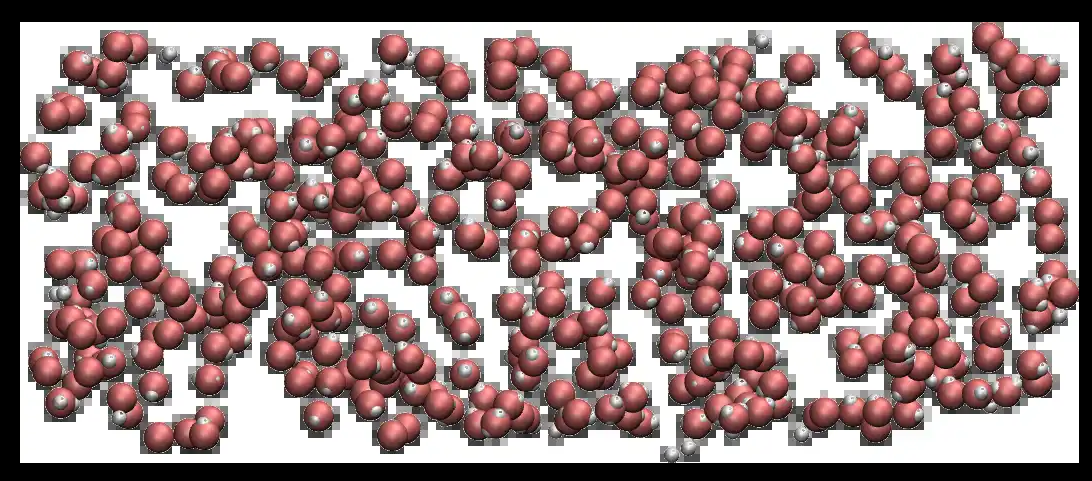
\includegraphics[width=\linewidth]{tutorials/level2/polymer-in-water/water_light.png}
\end{figure}

You can also open the temperature.dat and density.dat files
to ensure that the system converged toward an equilibrated
liquid system during the 50 ps of simulation:

\begin{figure}
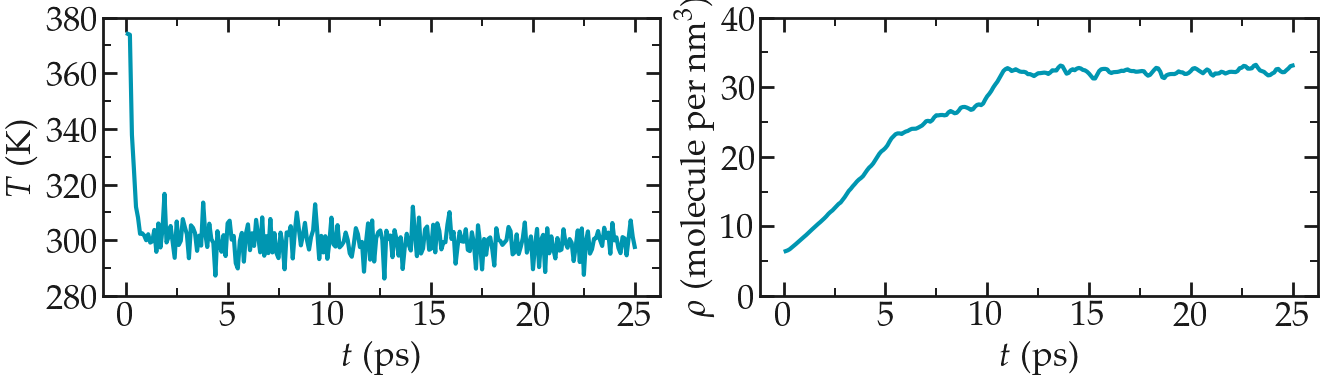
\includegraphics[width=\linewidth]{tutorials/level2/polymer-in-water/equilibration_H2O_light.png}
\end{figure}

Alternatively, you can \href{../../../../../inputs/level2/polymer-in-water/pureH2O/H2O.data}{download}
the water reservoir I have equilibrated and continue with
the tutorial.

\section{PEG molecule}

\noindent Now that the water box is ready, let us prepare the PEG
molecule in an empty box. Create a second folder next to pureH2O/, call it
singlePEG/, and create a new blank file called input.lammps
in it. Copy the same first lines as previously:

\begin{lcverbatim}
units real
atom_style full
bond_style harmonic
angle_style charmm
dihedral_style charmm
pair_style lj/cut/tip4p/long 1 2 1 1 0.105 12.0
kspace_style pppm/tip4p 1.0e-4
\end{lcverbatim}

\noindent Let us also add the \textit{special$\_$bonds} command to cancel the
Lennard-Jones interactions between the closest
atoms of a same molecule:

\begin{lcverbatim}
special_bonds lj/coul 0.0 0.0 0.5
\end{lcverbatim}

\noindent \begin{tcolorbox}[colback=mylightblue!5!white,colframe=mylightblue!75!black,title=About *special bonds*]
Usually, force fields like charmm are parametrized assuming that the first neighbors within a molecule do not
interact directly. Here, since we use 0.0 0.0 0.5, the first (for example C-O) and second (for example C-O-H) neighbors don't interact
with each other through LJ and Coulomb potentials, and therefore they only interact through direct bond interactions.
For the third neighbor (for example H-C-C-H), only half of the LJ and Coulomb interaction will be added.   
\end{tcolorbox}

\noindent Let us read the original positions for the atoms of the PEG molecule, as
well as the same parameter file as previously:

\begin{lcverbatim}
read_data init.data
include ../PARM.lammps
\end{lcverbatim}

\noindent \href{../../../../../inputs/level2/polymer-in-water/singlePEG/init.data}{Download}
the init.data file and save it in the singlePEG/ folder.
It contains the initial parameters of the PEG molecules
(atoms, bonds, charges, etc.) that was prepared using \href{https://github.com/simongravelle/PEGgenerator}{PEG generator}.
To make our life simpler later, let use use the exact same
box size for the PEG as for the water (the merging will be
simpler, see below). Open the previously generate H2O.data
file, and copy the 3 lines corresponding to the box
dimensions. In my case, its:

\begin{lcverbatim}
-21.64201909795004 21.64201909795004 xlo xhi
-8.115757161731125 8.115757161731125 ylo yhi
-8.115757161731125 8.115757161731125 zlo zhi
\end{lcverbatim}

\noindent Then, replace the box dimensions in the init.data file with
these 3 lines.
Let us print the atom positions and thermodynamic
information very frequently (because we anticipate that the
energy minimization will be short):

\begin{lcverbatim}
dump mydmp all atom 10 dump.lammpstrj
thermo 1
\end{lcverbatim}

\noindent Next, let us perform a minimisation of energy. Here, this
step is required because the initial configuration of the
PEG molecule is really far from equilibrium.

\begin{lcverbatim}
minimize 1.0e-4 1.0e-6 100 1000
\end{lcverbatim}

\noindent After the minimisation, the high resolution dump command is
cancelled, and a new dump command with lower frequency is
used (see below). We also reset the time to 0 with
\textit{reset$\_$timestep} command:

\begin{lcverbatim}
undump mydmp
reset_timestep 0
\end{lcverbatim}

\noindent The PEG is then equilibrated in the NVT ensemble (fix NVE +
temperature control = NVT). No box relaxation is required as
the PEG is in vacuum:

\begin{lcverbatim}
fix mynve all nve
fix myber all temp/berendsen 300 300 100
\end{lcverbatim}

\noindent Let us print the temperature in a file:

\begin{lcverbatim}
dump mydmp all atom 1000 dump.lammpstrj
dump_modify mydmp append yes
thermo 1000
variable mytemp equal temp
fix myat1 all ave/time 10 10 100 v_mytemp file temperature.dat
\end{lcverbatim}

\noindent The \textit{dump$\_$modify} ensures that the coordinates are written 
in the existing dump.lammpstrj file. 
Finally let us run the simulation for a very short time (10 ps):

\begin{lcverbatim}
timestep 1
run 10000
write_data PEG.data
\end{lcverbatim}

\noindent If you open the dump.lammpstrj file
using VMD, you can see the PEG molecule starting from
an extremely elongated and unrealistic shape, and 
gently equilibrating until reaching a reasonable state.

\begin{figure}
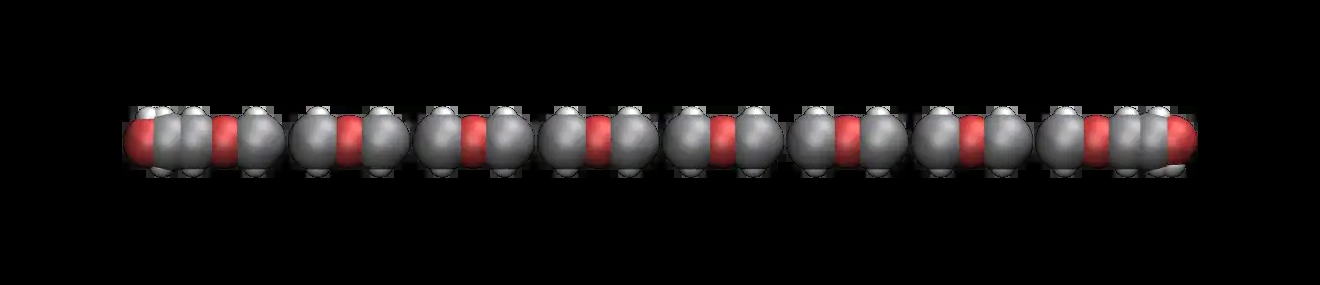
\includegraphics[width=\linewidth]{tutorials/level2/polymer-in-water/singlePEG-light.png}
\end{figure}

Alternatively, you can \href{../../../../../inputs/level2/polymer-in-water/singlePEG/PEG.data}{download}
the PEG molecule I have equilibrated and continue with the tutorial.

\section{Solvation of the PEG molecule}

\noindent Now, we merge the PEG molecule and the
water reservoir. We do it by:
\begin{itemize}
\item (1) importing both previously generated data files (PEG.data and H2O.data) into the same simulation,
\item (2) deleting the overlapping molecules, and 
\item (3) re-equilibrating the new system. 
\end{itemize}
Create a third folder alongside pureH2O/ and singlePEG/,
and call it mergePEGH2O/. Create a new blank file in it,
called input.lammps. Within input.lammps, copy the same first lines as
previously:

\begin{lcverbatim}
units real
atom_style full
bond_style harmonic
angle_style charmm
dihedral_style charmm
pair_style lj/cut/tip4p/long 1 2 1 1 0.105 12.0
kspace_style pppm/tip4p 1.0e-4
special_bonds lj/coul 0.0 0.0 0.5
\end{lcverbatim}

\noindent Then, import the two previously generated data files, as well as the same parameter file:

\begin{lcverbatim}
read_data ../singlePEG/PEG.data
read_data ../pureH2O/H2O.data add append
include ../PARM.lammps
\end{lcverbatim}

\noindent When using the \textit{read$\_$data} command more than once, one needs
to use the \textit{add append} keyword. When doing so, the
simulation box is initialized by the first \textit{read$\_$data} only, and the 
second \textit{read$\_$data} only imports additional atoms.
Let us create 2 groups to differentiate the PEG from the H2O:

\begin{lcverbatim}
group H2O type 1 2
group PEG type 3 4 5 6 7
\end{lcverbatim}

\noindent Water molecules that are overlapping with the PEG must be
deleted to avoid crashing:

\begin{lcverbatim}
delete_atoms overlap 2.0 H2O PEG mol yes
\end{lcverbatim}

\noindent Here the value of 2 Angstroms for the overlap cutoff was fixed arbitrarily,
and can be chosen through trial and error. If the cutoff is too small, the 
simulation will crash. If the cutoff it too long, too many water molecules will unnecessarily be deleted.
Finally, let us use shake to keep the water
molecules rigid, and use the NPT command to control the
temperature, as well as the pressure along the x axis:

\begin{lcverbatim}
fix myshk H2O shake 1.0e-4 200 0 b 1 a 1
fix mynpt all npt temp 300 300 100 x 1 1 1000
timestep 1.0
\end{lcverbatim}

\noindent The box dimension will only adjust along the x axis here.
Once more, let us dump the atom positions and a few
information about the evolution simulation:

\begin{lcverbatim}
dump mydmp all atom 100 dump.lammpstrj
thermo 100
variable mytemp equal temp
variable myvol equal vol
fix myat1 all ave/time 10 10 100 v_mytemp file temperature.dat
fix myat2 all ave/time 10 10 100 v_myvol file volume.dat
\end{lcverbatim}

\noindent Let us also print the total enthalpy:

\begin{lcverbatim}
variable myenthalpy equal enthalpy
fix myat3 all ave/time 10 10 100 v_myenthalpy file enthalpy.dat
\end{lcverbatim}

\noindent Finally, let us perform a short equilibration and print the
final state in a data file:

\begin{lcverbatim}
run 10000
write_data mix.data
\end{lcverbatim}

\noindent If you open the dump.lammpstrj file using VMD, you should
see that the box dimension slightly shrink along x.
The system looks like that:

\begin{figure}
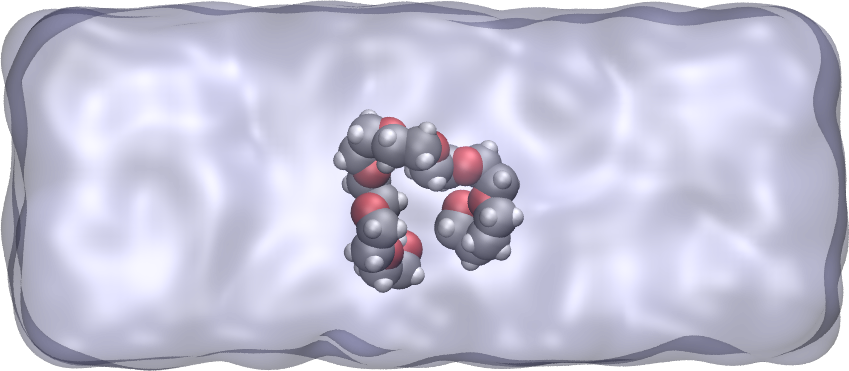
\includegraphics[width=\linewidth]{tutorials/level2/polymer-in-water/solvatedPEG_light.png}
\end{figure}

\section{Stretching the PEG molecule}

\noindent Here, a constant forcing is applied to the two ends of the
PEG molecule until it stretches. Create a new folder next
to the 3 previously created folders, call it pullonPEG/
and create a new input file in it called input.lammps.
First, let us create a variable containing the magnitude
of the force we are going to apply. The force magnitude is
chosen to be large enough to overcome the thermal
agitation and the entropic contribution from both water
and PEG molecules (it was chosen by trial and error). Copy
in the input file:

\begin{lcverbatim}
variable f0 equal 5 # kcal/mol/A # 1 kcal/mol/A = 67.2 pN
\end{lcverbatim}

\noindent Then, as previouly, copy:

\begin{lcverbatim}
units real
atom_style full
bond_style harmonic
angle_style charmm
dihedral_style charmm
pair_style lj/cut/tip4p/long 1 2 1 1 0.105 12.0
kspace_style pppm/tip4p 1.0e-4
special_bonds lj/coul 0.0 0.0 0.5
\end{lcverbatim}

\noindent Start the simulation from the equilibrated PEG + water
system, and include again the parameters:

\begin{lcverbatim}
read_data ../mergePEGH2O/mix.data
include ../PARM.lammps
\end{lcverbatim}

\noindent Then, let us create 4 atom groups: H2O and PEG (as
previously) as well as 2 groups containing one single atom
corresponding respectively to the oxygen atoms located at the
ends of the PEG molecule:

\begin{lcverbatim}
group H2O type 1 2
group PEG type 3 4 5 6 7
group oxygen_end1 id 65
group oxygen_end2 id 4
\end{lcverbatim}

\noindent Let us print again the atom positions in a dump:

\begin{lcverbatim}
dump mydmp all atom 1000 dump.lammpstrj
# write_dump all atom dump.lammpstrj
# dump myxtc xtc atom 1000 dump.xtc
\end{lcverbatim}

\noindent \begin{tcolorbox}[colback=mylightblue!5!white,colframe=mylightblue!75!black,title=Use less disk space by using the xtc format]

To generate smaller dump files, use the
compressed \textit{xtc} format. You can do it by commenting the
mydmp line and by uncommenting both the \textit{write$\_$dump} and
\textit{myxtc} lines. Note that \textit{xtc} files are compressed, and not readable
by humans, contrarily to the LAMMPS native format \textit{lammpstrj}. 
\end{tcolorbox}

\noindent Let us use a simple thermostating for all atoms 
and use shake for the rigid water molecules:

\begin{lcverbatim}
timestep 1
fix myshk H2O shake 1.0e-4 200 0 b 1 a 1
fix mynvt all nvt temp 300 300 100
\end{lcverbatim}

\noindent \begin{lcverbatim}
variable mytemp equal temp
fix myat1 all ave/time 10 10 100 v_mytemp file temperature.dat
variable x1 equal xcm(oxygen_end1,x)
variable x2 equal xcm(oxygen_end2,x)
variable delta_x equal abs(v_x1-v_x2)
fix myat2 all ave/time 10 10 100 v_delta_x file end-to-end-distance.dat
thermo 5000
\end{lcverbatim}

\noindent Finally, let us run the simulation for 10 ps (without
any external forcing):

\begin{lcverbatim}
run 10000
\end{lcverbatim}

\noindent This 10 ps serves as an extra small equilibration. In principle, 
it is not necessary as equilibration was properly performed during the 
previous step. Then, let us apply a forcing on the 2 oxygen atoms using 2
\textit{add$\_$force} commands, and run for 100 ps (for a total duration
of the simulation of 110 ps):

\begin{lcverbatim}
fix myaf1 oxygen_end1 addforce ${f0} 0 0
fix myaf2 oxygen_end2 addforce -${f0} 0 0
run 50000
\end{lcverbatim}

\noindent If you open the \textit{dump.lammpstrj} file using \textit{VMD}, you should
see this:

\begin{figure}
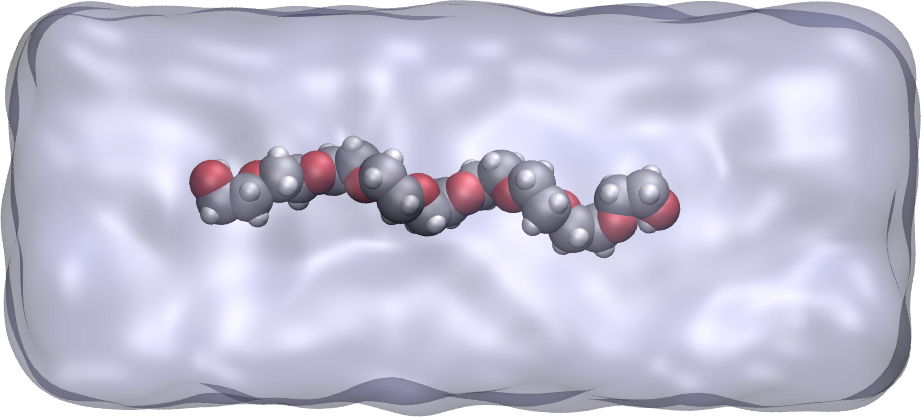
\includegraphics[width=\linewidth]{tutorials/level2/polymer-in-water/pulled_peg_light.png}
\end{figure}

The evolution of the end-to-end
distance over time shows the PEG adjusting
to the external forcing:

\begin{figure}
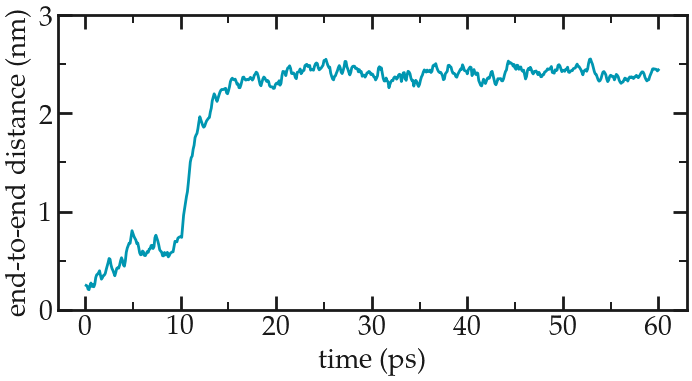
\includegraphics[width=\linewidth]{tutorials/level2/polymer-in-water/distance-light.png}
\end{figure}

\section{What now?}

\noindent Now that you have completed this relatively advanced molecular dynamics tutorials, and 
that all input scripts are working, I suggest you to mess around with the inputs and 
try to trigger warnings and error. The more warning and error you trigger from a working input, the 
easier it will be to solve future issue in your own input. 

\section{Going further with exercises}

\noindent \subsection{Generate a PEG-H2O mixture}

Use the same script and a similar procedure and create a
PEG-H2O mixture with several PEG molecules hydrated in a
cubic box.

\begin{tcolorbox}[colback=mylightblue!5!white,colframe=mylightblue!75!black,title=Hints]
LAMMPS has internal commands allowing to replicate
a molecule or a system.
There is no obligation to equilibrate the water molecules separately from the PEG,
as we did here. You can also create the water molecules directly around the PEG molcule
using the \textit{create$\_$atom} command.
\end{tcolorbox}

\noindent \subsection{End-to-end distance}

Create 2 simulations, one with a PEG molecule in vacuum, one
with a PEG molecule in water, and measure their respective
end-to-end equilibrium distance. PEG are hydrophilic and
form hbonds with water molecules, therefore, when immersed
in water, PEG molecules slightly unfold, which changes the
equilibrium end-to-end distance.

\subsection{Post-mortem analysis}

\noindent In today research, most data analyses are
done after the simulation is over, and it is important for
LAMMPS users to know how to do it.
Import the trajectory using Python, and re-extract the
end-to-end distance.

\begin{tcolorbox}[colback=mylightblue!5!white,colframe=mylightblue!75!black,title=Hints]
You can import \textit{lammpstrj} file using \textit{MDAnalysis} in \textit{Python}:
\begin{lcverbatim}
u = mda.Universe("dump.lammpstrj", format = "LAMMPSDUMP")
\end{lcverbatim}

\noindent \end{tcolorbox}


\chapter{Nanosheared electrolyte}
\label{sheared-confined-label}

\vspace{-1cm} \noindent \textcolor{graytitle}{\textit{{\Large Aqueous NaCl solution sheared by two walls}}\vspace{0.5cm} }

\noindent \hspace{-0.45cm}\begin{wrapfigure}{r}{4cm}
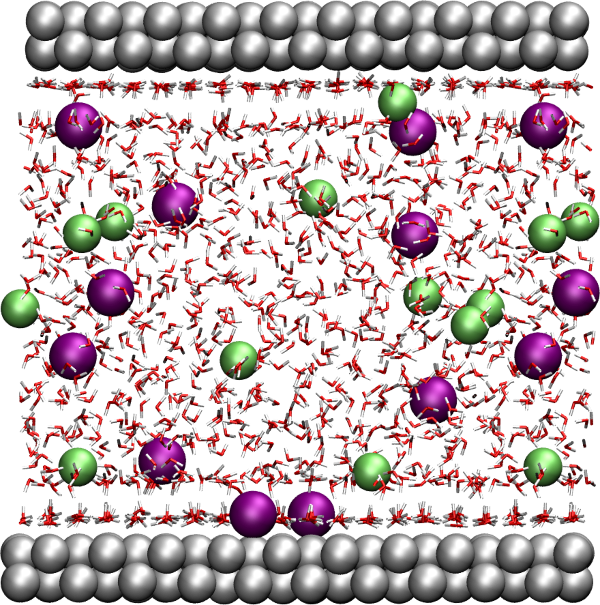
\includegraphics[width=4cm]{tutorials/level2/nanosheared-electrolyte/nanoconfined-electrolyte-light.png}
\end{wrapfigure}

\noindent The objective of this tutorial is to
simulate an electrolyte sheared by two walls. Some properties
of the sheared fluid, such as the time-averaged velocity profile
will be extracted. 
This tutorial illustrates the important aspects of
combining a fluid and a solid in the same simulation.

\section{System generation}

\noindent Create a new folder called \textit{SystemCreation/}. Within \textit{SystemCreation/},
open a blank file called \textit{input.lammps}, and copy 
the following lines into it:

\begin{lcverbatim}
# LAMMPS input file
units real
atom_style full
bond_style harmonic
angle_style harmonic
pair_style lj/cut/tip4p/long 1 2 1 1 0.1546 12.0
kspace_style pppm/tip4p 1.0e-4
\end{lcverbatim}

\noindent These lines are used to define the most basic parameters,
including the \textit{atom}, \textit{bond}, and \textit{angle} styles, as well as 
interaction potential (here Lennard Jones with cut-off and long 
range Coulombic) and long range solver (here PPPM). 
These lines are relatively similar to the 
previous tutorial (\ref{all-atoms-label}).

\begin{tcolorbox}[colback=mylightblue!5!white,colframe=mylightblue!75!black,title=About lj/cut/tip4p/long pair style]
The lj/cut/tip4p/long pair style is similar to the conventional 
Lennard Jones + Coulomb interaction, except that it is made specifically 
for four point water model (tip4p). The atom of the water model
will be type 1 (O) and 2 (H). All the other atoms of the simulations 
are treated \textit{normally} with long range coulomb interaction.
\end{tcolorbox}

\noindent Let us create the box:

\begin{lcverbatim}
# ------------- System definition
lattice fcc 4.04
region box block -4 4 -4 4 -13 13
create_box 5 box &
\end{lcverbatim}

\noindent The \textit{lattice} command defines the unit
cell. Here, the face-centered cubic (fcc) lattice with a scale factor of
4.04 has been chosen for the future positioning of the atoms
of the walls.

The \textit{region} command defines a geometric
region of space. By choosing \textit{xlo=-4} and \textit{xhi=4}, and
because we have previously chosen a lattice with scale
factor of 4.04, the region box extends from -16.16 Å to 16.16 Å.

The \textit{create$\_$box} command creates a simulation box with 5 types of atoms in
the simulation. This command extends over 6 lines thanks to the
$\&$ character. The second and third lines are used to
specify that the simulation contains 1 type of bond and 1
type of angle (both required by the water molecule). The parameters of
these bond and angle constraints will be given later. The
three last lines are for memory allocation.
Note that 5 atom types are needed for respectively the oxygen and hydrogen
of the water molecules, the two types of ions ($\text{Na}^+$, $\text{Cl}^-$), and the
single atom type of the walls.

Now, we can add atoms to the system. First, let us create two
sub-regions corresponding respectively to the two solid
walls, and create a larger region from the union of the two
regions. Then, let us create atoms of type 5 (the wall) within the two
regions:

\begin{lcverbatim}
# create the walls
region rbotwall block -4 4 -4 4 -12 -10
region rtopwall block -4 4 -4 4 10 12
region rwall union 2 rbotwall rtopwall
create_atoms 5 region rwall
\end{lcverbatim}

\noindent Atoms will be placed at the positions of the previously
defined lattice.
In order to add the water molecules, we first need to
download the \href{../../../../../inputs/level2/nanosheared-electrolyte/TIP4P2005.txt}{TIP4P2005.txt}
file and place it in \textit{SystemCreation/}. It contains all the
necessary information about the water molecule, such as
atom positions, bonds, and the angle.

Add the following lines
to input.lammps:

\begin{lcverbatim}
# create the fluid
region rliquid block -4 4 -4 4 -9 9
molecule h2omol ../TIP4P2005.txt
lattice sc 4.04
create_atoms 0 region rliquid mol h2omol 482793
\end{lcverbatim}

\noindent Withing the last four lines, a \textit{region} named \textit{rliquid} for depositing the water molecules is created based
on the last defined lattice, which is \textit{fcc 4.04}. 
The \textit{molecule} command opens up the \textit{TIP4P2005.txt} file, and names
the associated molecule \textit{h2omol}.
A new simple cubic lattice is defined in order to place the water
molecules on it, with a distance of 4.04 Ångstroms between
each water molecule. Note that the new lattice replaces the
previous one, as LAMMPS reads a script from top to bottom.
Note that the distance of 4.04 Ångstroms is larger than the typical
equilibrium distance between water molecules in a liquid,
but this will allow us to insert ions more safely (see below). 
Finally, molecules are created on the sc lattice by the \textit{create$\_$atoms} command. The
first parameter is '0' because we use the atom id from the
\textit{TIP4P2005.txt} file. The number \textit{482793} is a seed that is
required by LAMMPS, it can be any positive integer.
Let us create 20 ions (10 $\text{Na}^+$ and 10 $\text{Cl}^-$)
in between the water molecules:

\begin{lcverbatim}
# create the ions
create_atoms 3 random 10 52802 rliquid overlap 0.3 maxtry 500
create_atoms 4 random 10 90182 rliquid overlap 0.3 maxtry 500
set type 3 charge 1.0
set type 4 charge -1.0
\end{lcverbatim}

\noindent Each \textit{create$\_$atoms} command will add 10 ions at random positions
within the 'rliquid' region. Feel free to increase or decrease the salt
concentration by changing the number of desired ions.
The charges of the newly added ions are specified by the two \textit{set} commands.
To keep the system charge neutral, always insert the same number of 
$\text{Na}^+$ and $\text{Cl}^-$ (unless of course there are other charges in the system).
We need to define the parameters of the simulation: the mass
of the 6 atoms (O, H, $\text{Na}^+$, $\text{Cl}^-$, and wall), the
pairwise interaction parameters (here the parameters for the
Lennard-Jones potential), and the bond and angle parameters.
Copy the following line into input.lammps:

\begin{lcverbatim}
# settings
include ../PARM.lammps
\end{lcverbatim}

\noindent Create a new text file, call it \textit{PARM.lammps}, and copy it
next to the \textit{SystemCreation/} folder. Copy the following lines
into PARM.lammps:

\begin{lcverbatim}
# Parameter file
mass 1 15.9994 # water
mass 2 1.008 # water
mass 3 28.990 # ion
mass 4 35.453 # ion
mass 5 26.9815 # wall
pair_coeff 1 1 0.185199 3.1589 # water
pair_coeff 2 2 0.0 0.0 # water
pair_coeff 3 3 0.04690 2.4299 # ion
pair_coeff 4 4 0.1500 4.04470 # ion
pair_coeff 5 5 11.697 2.574 # wall
bond_coeff 1 0 0.9572 # water
angle_coeff 1 0 104.52 # water

\end{lcverbatim}

\noindent Each \textit{mass} command assigns a mass in grams/mole to an atom type. Each
\textit{pair$\_$coeff} assigns respectively the depth of the potential
(in Kcal/mole), and the distance (in Ångstrom) at which the
particle-particle potential energy is 0.

\begin{tcolorbox}[colback=mylightblue!5!white,colframe=mylightblue!75!black,title=About the parameters]
The parameters for water
correspond to the TIP4P/2005 water model, and the parameters
for $\text{Na}^+$ and $\text{Cl}^-$  are
taken from the CHARMM-27 force field.
\end{tcolorbox}

\noindent Only pairwise interaction between atoms of
identical type were assigned. By default, LAMMPS calculates
the pair coefficients for the interactions between atoms
of different types (i and j) by using geometrical
average: $\epsilon_{ij} = \epsilon_i + \epsilon_j)/2$, 
$\sigma_{ij} = (\sigma_i + \sigma_j)/2.$
Other rules for cross coefficients can be set with the
\textit{pair$\_$modify} command, but for the sake of simplicity,
let us keep the default option here.
The bond coefficient (here for the O-H bond of the water
molecule) sets respectively the energy of the harmonic
potential and the equilibrium distance in Ångstrom. The
value is '0' for the energy, because we are going to use a
rigid model for the water molecule. The shape of the
molecule will be preserved later by the shake algorithm.
Similarly, the angle coefficient (here for the H-O-H angle
of the water molecule) sets the energy of the harmonic
potential (also 0) and the equilibrium angle is in degree.
Finally, add the following lines to the input file:

\begin{lcverbatim}
# run
run 0
write_data system.data
write_dump all atom dump.lammpstrj
\end{lcverbatim}

\noindent With \textit{run 0}, the simulation will run for 0 step,
enough for creating the system and saving the final state.
The \textit{write$\_$data} finally creates a file named \textit{system.data}
containing all the information required to restart the
simulation from the final configuration generated by this
input file.
The \textit{write$\_$dump} command print the final
positions of the atoms, and can be used with VMD or ovito
to visualize the system.
This input script is ready to be ran with LAMMPS. When the
run is over, open the log file and make sure that atoms have
been created (look for lines like 'Created 3648 atoms'), or
just look at the dump file with VMD:

\begin{figure}
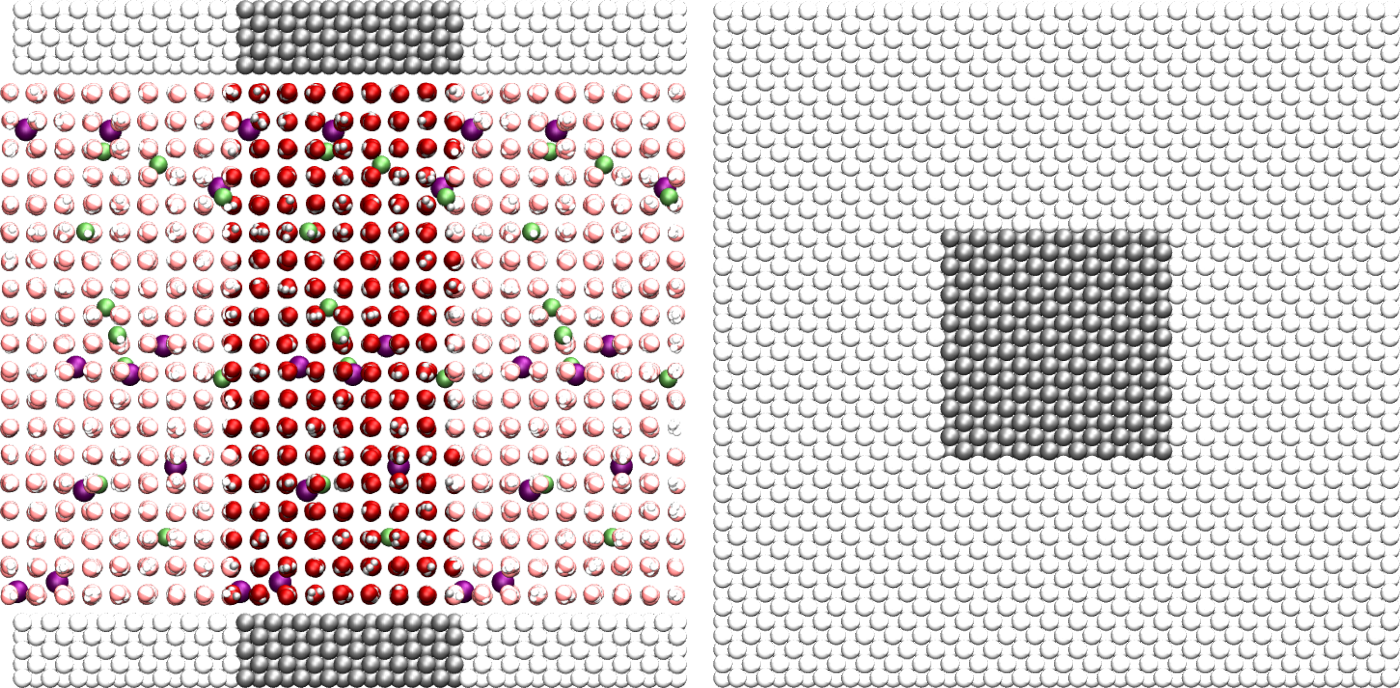
\includegraphics[width=\linewidth]{tutorials/level2/nanosheared-electrolyte/systemcreation-light.png}
\end{figure}

Always check that your system has been correctly created
by showing the periodic images. Atomic defects often
occur at the boundary.

\section{Energy minimization}

\noindent \begin{tcolorbox}[colback=mylightblue!5!white,colframe=mylightblue!75!black,title=Why is energy minimization necessary?]
It is clear from the way the system has been created that
the atoms are not at equilibrium distances from each
others. Indeed, some of the ions added using the \textit{create$\_$atoms}
commands are too close to the water molecules.
If we were to start a molecular dynamics
simulation now (i.e. solve the equations of motion) with
a conventional timestep of 1 femto-seconds, the atoms
would exert huge forces on each others, accelerate
brutally, and the simulation would fail.
\end{tcolorbox}

\noindent \begin{tcolorbox}[colback=mylightblue!5!white,colframe=mylightblue!75!black,title=Dealing with overlapping atoms]
MD simulations failing due to overlapping atoms are
extremely common, and I can almost guarantee that you
will face a similar issue at some point. If it occurs,
you can either
\begin{itemize}
\item delete the overlapping atoms using the \textit{delete$\_$atoms} command of LAMMPS, or
\item move the atoms to more reasonable distances before the simulation starts.
\end{itemize}
\end{tcolorbox}

\noindent Let us move the atoms and place them
in more energetically favorable positions before starting the simulation.
To perform the energy minimization with our system, let us
create a new folder named Minimization/, and create a new
input file named input.lammps in it. The first lines will be
very similar to the previous input file:

\begin{lcverbatim}
# Initialisation
boundary p p p
units real
atom_style full
bond_style harmonic
angle_style harmonic
pair_style lj/cut/tip4p/long 1 2 1 1 0.1546 12.0
kspace_style pppm/tip4p 1.0e-4
# System definition
read_data ../SystemCreation/system.data
# settings
include ../PARM.lammps
\end{lcverbatim}

\noindent The only difference with the previous input is that, instead
of creating a new box and new atoms, we open the
previously created file \textit{system.data} located in \textit{SystemCreation/}.
\textit{system.data} contains the definition of the simulation box and the positions of the atoms.
Next, let us create a group for the water:

\begin{lcverbatim}
group gH2O type 1 2
\end{lcverbatim}

\noindent Creating groups will allow us to apply different dynamics and constraints to the
liquid and to the walls.
Let us also print the atoms positions in a dump file:

\begin{lcverbatim}
dump mydmp all atom 1000 dump.lammpstrj
\end{lcverbatim}

\noindent Now, we can include the most important commands for the
minimization:

\begin{lcverbatim}
fix mynve all nve/limit 0.1
fix myber all temp/berendsen 1 1 1
\end{lcverbatim}

\noindent The fix \textit{nve/limit} performs constant NVE integration to
update positions and velocities of the atoms at each
timestep, but limit the maximum motion an atom can do at
every timestep. The temp/berendsen fix rescales the
velocities of the atoms every timestep in order to reset the
temperature.

Since we want to perform a minimization step, both initial
and final temperatures have been chosen equal to 1K. The
third parameter is the damping factor, in time units, which
determines how rapidly the temperature is relaxed. Such
damping factor of 1 fs would be too small for a regular
molecular dynamics simulation, but is acceptable for a
minimization step during which we just want the atoms to
move slightly from their initial positions.

If we were to run the simulation as it is, it would fail
because nothing maintains the shape of the water molecules
(and the bond and angle energies are equal to 0). Let us use
the shake algorithm in order to maintain the shape of the
molecules. In addition, let us add a fix \textit{recenter} in order
to maintain the system centered in the middle of the box in
the \textit{z} direction:

\begin{lcverbatim}
fix myshk gH2O shake 1.0e-4 200 0 b 1 a 1
fix myrct all recenter NULL NULL INIT
\end{lcverbatim}

\noindent Fix recenter has no influence on the dynamics, but will keep the system in the 
center of the box, which makes the visualization easier.
Finally, let us choose a small timestep (because we
anticipate that the atoms are initially too close to each
others) and run for 10000 steps:

\begin{lcverbatim}
timestep 0.5
thermo 50
run 10000
write_data system.data
\end{lcverbatim}

\noindent When running the input.lammps file, you should see that the
total energy of the system decreases as expected (fifth
colum):

\begin{lcverbatim}
Step   Temp          E_pair         E_mol          TotEng         Press     
50   3.492673      -107825.17      0             -107786.32     -19733.701    
100   2.6260191     -108926.18      0             -108896.97     -20225.668    
150   2.2025292     -109692.83      0             -109668.34     -20319.962 
(...)
9800   1.0233163     -120975.23      0             -120963.85     -12590.345    
9850   1.022532      -120988.11      0             -120976.74     -12582.803    
9900   1.0222164     -121000.48      0             -120989.11     -12573.028    
9950   1.0215887     -121012.78      0             -121001.42     -12562.843    
10000   1.0206449     -121024.53      0             -121013.18     -12551.132 
\end{lcverbatim}

\noindent You can easily import log file into \textit{Python} using the
\href{https://pypi.org/project/lammps-logfile/}{LAMMPS logfile} tool, and plot the thermodynamic quantities as a function 
of the time:

\begin{figure}
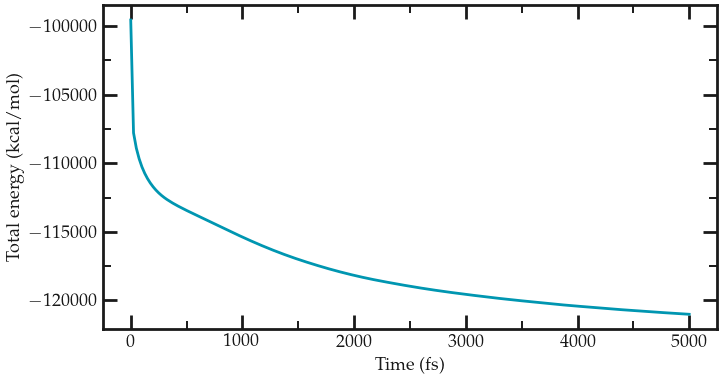
\includegraphics[width=\linewidth]{tutorials/level2/nanosheared-electrolyte/minimization-light.png}
\end{figure}

If you look at the trajectory using VMD, you will see some
of the atoms (the one that where initially in a problematic
position) slightly move from each others, as seen in \href{https://youtu.be/JWGZnFN4TOo}{this video}.

\section{System equilibration}

\noindent Now, let us properly equilibrate the system by letting both
fluid and piston relax at ambient temperature.
Create a new folder called \textit{Equilibration/}, create a new
input file in it, and add the following lines:

\begin{lcverbatim}
# Initialisation
boundary p p p
units real
atom_style full
bond_style harmonic
angle_style harmonic
pair_style lj/cut/tip4p/long 1 2 1 1 0.1546 12.0
kspace_style pppm/tip4p 1.0e-4
# System definition
read_data ../Minimization/system.data
# Simulation settings
include ../PARM.lammps
# Define groups
group gH2O type 1 2
group gNa type 3
group gCl type 4
group gliquid type 1 2 3 4
group gwall type 5
region rtop block INF INF INF INF 0 INF
region rbot block INF INF INF INF INF 0
group gtop region rtop
group gbot region rbot
group gwalltop intersect gwall gtop
group gwallbot intersect gwall gbot
\end{lcverbatim}

\noindent Here, several groups have been defined in order to differentiate
between solid, liquid (salt+water), $\text{Na}^+$, etc. (although
not all of them are used). In addition, groups containing only the
top wall (gwalltop) and the bottom wall (gwallbot) have been
created using the intersect keyword: the intersection
between all the atom on the top part of the box (gtop) and
all the atom of type 5 (gwall) corresponds to the top wall.
Then, add the following lines for the visualisation :

\begin{lcverbatim}
# visualisation
dump mydmp all atom 1000 dump.lammpstrj
thermo 50
variable walltopz equal xcm(gwalltop,z)
variable wallbotz equal xcm(gwallbot,z)
variable deltaz equal v_walltopz-v_wallbotz
fix myat1 all ave/time 10 10 100 v_deltaz file interwall_distance.dat
\end{lcverbatim}

\noindent The two variables allow to extract the centers of mass of
the two walls, respectively, and the deltaz variable
calculates the difference between the two centers of mass.
Finally, add the end of the input:

\begin{lcverbatim}
# Dynamics
fix mynve all nve
compute tliq gliquid temp
fix myber1 gliquid temp/berendsen 300 300 100
fix_modify myber1 temp tliq
compute twall gwall temp
fix myber2 gwall temp/berendsen 300 300 100
fix_modify myber2 temp twall
fix myshk gH2O shake 1.0e-4 200 0 b 1 a 1
fix myrct all recenter NULL NULL INIT
timestep 1.0
run 20000
write_data system.data
\end{lcverbatim}

\noindent The main differences with the previous step (minimize) are
the timestep of 1 fs instead of 0.5 fs, the thermostat that imposes a temperature of 300 K, for which the
fluid is expected to behave as a liquid, and the two thermostats are used instead of one:
one for the fluid, one for the solid (the use of \textit{fix$\_$modify} ensures
that the right temperature is used by the temp/berenden).

Run the input script. Note, I am running on 4 CPU cores using:

\begin{lcverbatim}
mpirun -np 4 lmp -in input.lammps
\end{lcverbatim}

\noindent To complete the 20000 steps (20 ps), it takes about 6 minutes. The duration 
may differ on your computer.
The distance between the two walls
reduces until it reaches an equilibrium value (see the data
printed by \textit{fix myat1}):

\begin{figure}
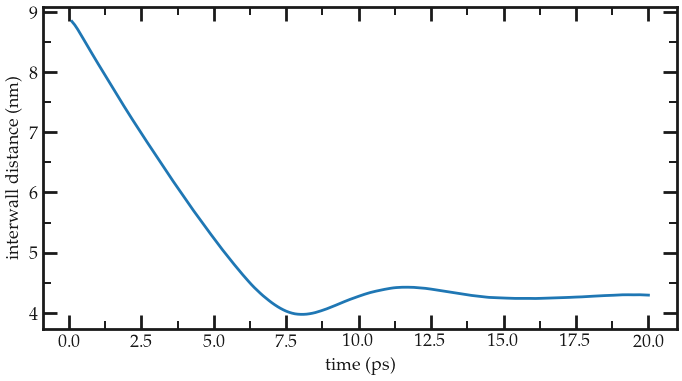
\includegraphics[width=\linewidth]{tutorials/level2/nanosheared-electrolyte/equilibration-light.png}
\end{figure}

Note that for actual reseach, it is recommended to run this equilibration step for longer times
to make sure that proper equilibration was reached. Here, since the slowest
process is the ionic diffusion, the equilibration 
should be longer than the typical diffusion time of the ions over the 
size of the pore (~3 nm), i.e. of the order of the nanosecond.

\section{Imposed shearing}

\noindent From the equilibrated configuration, let us impose the
motion of the two walls in order to shear the electrolyte.
In a new folder called \textit{Shearing/},
create a new input that starts like the previous ones:

\begin{lcverbatim}
# Initialisation
boundary p p p
units real
atom_style full
bond_style harmonic
angle_style harmonic
pair_style lj/cut/tip4p/long 1 2 1 1 0.1546 12.0
kspace_style pppm/tip4p 1.0e-4
# System definition
read_data ../Equilibration/system.data
change_box all z final -40 40
# Simulation settings
include ../PARM.lammps
# Groups
group gH2O type 1 2
group gNa type 3
group gCl type 4
group gliquid type 1 2 3 4
group gwall type 5
region rtop block INF INF INF INF 0 INF
region rbot block INF INF INF INF INF 0
group gtop region rtop
group gbot region rbot
group gwalltop intersect gwall gtop
group gwallbot intersect gwall gbot
# Dynamics
fix mynve all nve
compute tliq gliquid temp/partial 0 1 1
fix myber1 gliquid temp/berendsen 300 300 100
fix_modify myber1 temp tliq
compute twall gwall temp/partial 0 1 1
fix myber2 gwall temp/berendsen 300 300 100
fix_modify myber2 temp twall
fix myshk gH2O shake 1.0e-4 200 0 b 1 a 1
fix myrct all recenter NULL NULL INIT
\end{lcverbatim}

\noindent The main difference with the previous \textit{equilibration} step, so far, is
the use of temperature \textit{compute} with \textit{temp/partial 0 1 1} options.
This is meant to exclude the \textit{x} coordinate from the thermalisation, which is 
important since a large velocity will be imposed along \textit{x}. Another difference is the
\textit{change$\_$box} command used to reduce the size of the box along \textit{z} (otherwise there 
is too much unecessary vacuum).
Then, let us impose the motion of the two walls:

\begin{lcverbatim}
fix mysf1 gwalltop setforce 0 NULL NULL
fix mysf2 gwallbot setforce 0 NULL NULL
velocity gwallbot set -20e-5 NULL NULL
velocity gwalltop set 20e-5 NULL NULL
\end{lcverbatim}

\noindent The \textit{setforce} commands cancel the forces on a group of atoms at
every timestep, so the atoms of the group do not
experience any force from the rest of the system. In absence of force
acting on those atoms, they will conserve their initial velocity.
The \textit{velocity} commands act only once and impose
the velocity of the atoms of the groups \textit{gwallbot} and \textit{gwalltop}, respectively.
Finally, let us dump the atom positions, extract the
velocity profile using the ave/chunk command, extract the
force applied on the walls, and then run for 20 ps (feel free to increase the duration 
for more accurate velocity profile):

\begin{lcverbatim}
# vizualisation
dump mydmp all atom 5000 dump.lammpstrj
thermo 500
thermo_modify temp tliq
compute cc1 gliquid chunk/atom bin/1d z 0.0 1.0
fix myac1 gliquid ave/chunk 10 1500 20000 cc1 vx file vel.profile.dat
compute cc2 gwall chunk/atom bin/1d z 0.0 1.0
fix myac2 gwall ave/chunk 10 1500 20000 cc2 vx file vel.solid.dat
fix myat1 all ave/time 10 100 1000 f_mysf1[1] f_mysf2[1] file forces.dat
timestep 1.0
run 20000
write_data system.data
\end{lcverbatim}

\noindent Note that a duration of 20 ps is too short to measure meaningfull quantities.
If you computer allows it, use 200 ps instead.
The averaged velocity profile (with a 200 ps run) is the following:

\begin{figure}
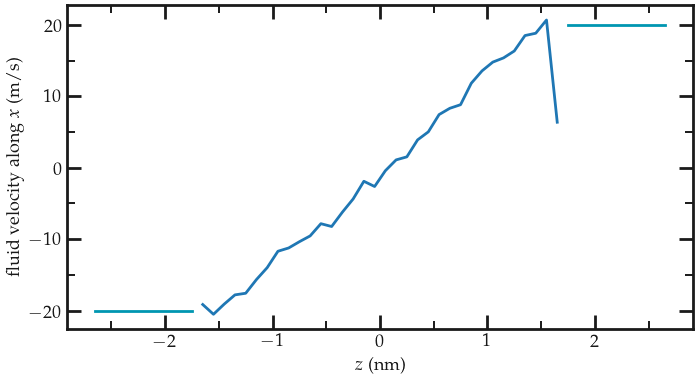
\includegraphics[width=\linewidth]{tutorials/level2/nanosheared-electrolyte/shearing-light.png}
\end{figure}

From the force applied by the fluid on the solid, one can
extract the stress within the fluid, which allows one to
measure its viscosity $\dot{\eta}$ 
according to \href{https://pure.tudelft.nl/ws/portalfiles/portal/89280267/PhysRevFluids.6.034303.pdf}{gravelle2021}:
$\eta = \tau / \dot{\gamma}$ where $\tau$
is the stress applied by the fluid on the shearing wall, and
$\dot{\gamma}$ the shear rate (which is imposed
here). Here the shear rate is approximatively 6.25e9
s-1, and using a surface area of 1e-17 m2, I
get a viscosity for the fluid equal to 2.25 mPa.s
The viscosity calculated at such high shear rate may
differ from the bulk value. In general, it is recommanded to use a lower
value for the shear rate. Note that for lower shear rate, the ratio noise-to-signal
is larger, and longer simulations must be performed.
Also note that the viscosity of a fluid next to a solid surface is
typically larger than in bulk due to interaction with the
walls. Therefore one expect the present simulation to return 
a viscosity that is slightly larger than what would be measured with 
the fluid alone.

\section{Going further with exercises}

\noindent \subsection{Density profiles}

Perform an equilibrium simulation, and extract both density
profiles and diffusion coefficients in all 3 directions of
space.
Hint: in general, data extraction can ne done either (1)
using the internal LAMMPS commands (e.g. variable/compute
+ fix ave/time), or (2) using a post-processing analysis
tool (e.g. Python).

\subsection{Poiseuille flow}

\noindent Instead of inducing shearing using the walls, induce a flow
of the liquid in the direction tangential to the walls, and
extract the the velocity profile.
Advice: the forcing must be chosen with care. If too
large, the system will be strongly out-of-equilibrium. If
too small, no net velocity will be measured because of
the thermal noise.
Question: Is the velocity profile you obtain consistent with
Poiseuille's predictions?


\chapter{Reactive silicon dioxide}

\vspace{-1cm} \noindent \textcolor{graytitle}{\textit{{\Large Simulating a chemically reactive structure}}\vspace{0.5cm} }

\noindent \hspace{-0.45cm}\begin{wrapfigure}{r}{4cm}
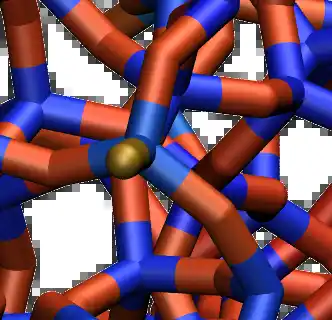
\includegraphics[width=4cm]{tutorials/level3/reactive-silicon-dioxide/SiO_gif_light.png}
\end{wrapfigure}

\noindent The objective of this tutorial is to use a molecular
dynamics system made of silicon dioxide (SiO2), and deform 
it until it breaks. The reactive force field \textit{reaxff} is used, and 
a particular attention is given to the evolution of the charges
of the atoms during the deformation of the structure. 

\section{Relax the structure}

\noindent Create a folder, name it RelaxSilica/, and \href{../../../../../inputs/level3/reactive-silicon-dioxide/RelaxSilica/silica.data}{download}
the initial topology of a small amorphous silica structure.
The system was created by temperature annealing using another force field 
(\href{../../../../../inputs/level3/reactive-silicon-dioxide/CreateSilica/SiO.1990.vashishta}{vashishta}), therefore the structure is slightly
different to what is expected from the reaxff force field. 
For instance, the average bond lengths, angles, and charges 
are likely to be different, and the structure needs 
to be relaxed again using reaxff. 
If you are interested, the input file used for creating the initial topology is 
available \href{../../../../../inputs/level3/reactive-silicon-dioxide/CreateSilica/input.lammps}{here}, but its description is not part of this tutorial.
The Atoms section of the \textit{silica.data} file starts like that:

\begin{lcverbatim}
Atoms # full
132 15 2 -0.55 1.722106654667303 6.0790786378597526 5.627968948336774 -6 4 -5
172 20 1 1.1 5.755393150671698 3.31535305846982 1.0501387543709164 4 3 2
231 26 2 -0.55 5.617126717910301 7.487471864752421 1.963810241571427 -16 8 -3
54 6 2 -0.55 4.060884959755418 1.6283060986470597 4.297860218329581 -7 -4 3
174 20 1 1.1 2.9926597997825395 2.0364512736354192 0.7520371846065788 -2 -6 -7
180 20 2 -0.55 3.18438907446254 2.5721052475107857 6.622363526485664 0 -12 1
121 14 2 -0.55 5.537222937373211 1.456250286791573 6.343752399466858 -9 -12 -4
111 13 1 1.1 1.7279273441891305 7.28674041911877 6.669158065545038 6 -10 -2
51 6 2 -0.55 5.366932941422638 4.1504125630630435 2.3740196532457105 0 -1 -3
202 23 2 -0.55 7.313845702241226 3.321272888336706 3.777618751313188 0 5 -13
215 24 2 -0.55 6.690317849940269 5.754543737004929 4.103252634559489 -6 2 0
183 21 1 1.1 1.777618482333677 6.145548171417662 3.999369841948803 -5 -5 -3
95 11 2 -0.55 4.561227581704491 2.3474960588346616 0.6330321107351076 -1 -6 3
105 12 2 -0.55 5.0710009155644125 3.8511969818510208 5.143556706337486 -1 0 5
(...)
\end{lcverbatim}

\noindent Due to the use of vashishta force field for creating the initial configuration,
all silicon atoms have the same charge q = 1.1e,
and all oxygen atoms the charge q = -0.55e. This is common to most
classical force field. Let us keep that in mind before we start using \textit{reaxff}.
The first step is to relax the structure, which we are gonna do using molecular
dynamics. To make sure that the system equilibrates nicely, let us track the
changes in our system over time. 
Create an input file called input.lammps in RelaxSilica/, and copy in it: 

\begin{lcverbatim}
units real
atom_style full
read_data silica.data
mass 1 28.0855 # Si
mass 2 15.999 # O
\end{lcverbatim}

\noindent So far, the input is very similar to what is seen in the other tutorials here,
with some basic parameters being defined (\textit{units}, \textit{atom$\_$style} and \textit{masses}), and 
the data file being imported by the \textit{read$\_$data} command.
Now let us enter 3 crucial lines:

\begin{lcverbatim}
pair_style reaxff NULL safezone 3.0 mincap 150
pair_coeff * * reaxCHOFe.ff Si O
fix myqeq all qeq/reaxff 1 0.0 10.0 1.0e-6 reaxff maxiter 400
\end{lcverbatim}

\noindent Here, the reaxff \textit{pair$\_$style} is used with no control file, and the \textit{safezone} and \textit{mincap}
keywords have been added for memory allocation issue. If not there, the segmentation
faults and bondchk failed errors sometimes occur.
The \textit{pair$\_$coeff} uses the \href{../../../../../inputs/level3/reactive-silicon-dioxide/RelaxSilica/reaxCHOFe.ff}{reaxCHOFe.ff} file which is assumed to be saved in the
same folder as the input. The atoms of type 1 are set as silicon (Si),
and type 2 as oxygen (O) in order to be consistent with the data file and
mass definition.
Finally, the fix \textit{qeq/reaxff} is used to perform charge equilibration every timestep. The values 0 and 10.0
are low and high cutoffs, respectively, and $1.0 \text{e}-6$ a tolerance. Finally, maxiter sets
a limit to the number of attempt to equilibrate the charge. 

\begin{tcolorbox}[colback=mylightblue!5!white,colframe=mylightblue!75!black,title=Note]
If the charge does not
properly equilibrate despite the 400 attempts, a warning will appear. Such warning
are likely to appear if the initial charges are too far from equilibrium values. 
\end{tcolorbox}

\noindent Then, let us use some (familiar) commands controlling the building of the 
neighbor lists. Let us also print thermodynamic information, the charge of both atom types,
and create a dump file for visualization.

\begin{lcverbatim}
neighbor 0.5 bin
neigh_modify every 5 delay 0 check yes 
group grpSi type 1
group grpO type 2
variable totqSi equal charge(grpSi)
variable totqO equal charge(grpO)
variable nSi equal count(grpSi)
variable nO equal count(grpO)
variable qSi equal v_totqSi/${nSi}
variable qO equal v_totqO/${nO}
dump dmp all custom 100 dump.lammpstrj id type q x y z
thermo 10
thermo_style custom step temp etotal press vol v_qSi v_qO
\end{lcverbatim}

\noindent Let us perform a very short run using anisotropic NPT command
and relax the density of the system. 

\begin{lcverbatim}
velocity all create 300.0 3482028
fix mynpt all npt temp 300.0 300.0 10 aniso 1.0 1.0 100
timestep 0.5
run 2000
\end{lcverbatim}

\noindent \begin{tcolorbox}[colback=mylightblue!5!white,colframe=mylightblue!75!black,title=Note]
Here, I choose values of 10 fs for the temperature damping parameter and 100 fs
for the pressure. These choices were made to reach equilibrium faster and 
allow very short run to be performed. For an actual simulation (and not a tutorial),
longer equilibration and larger damping times should be used (100 fs and 1000 fs
for temperature and pressure respectively are usually used for atomic systems).
\end{tcolorbox}

\noindent As the simulation runs, you can see that the charges of the atoms are fluctuating,
as the atoms adjust themselves to the topology:

\begin{figure}
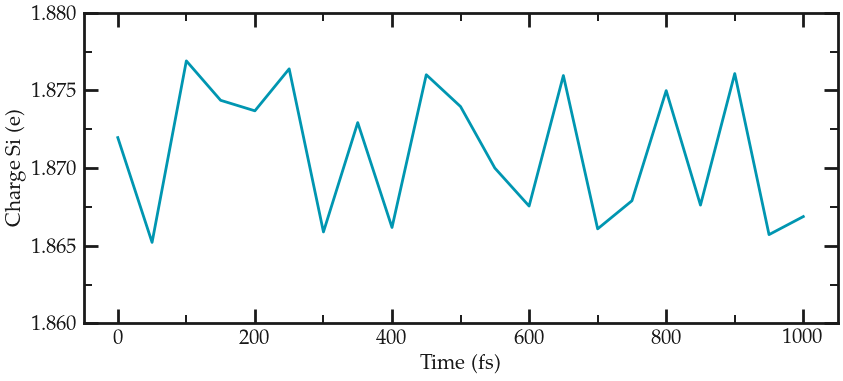
\includegraphics[width=\linewidth]{tutorials/level3/reactive-silicon-dioxide/average-charge-light.png}
\end{figure}

Moreover, and because each atom adopts its own fluctuating charge value,
the charges are distributed around a mean value:

\begin{figure}
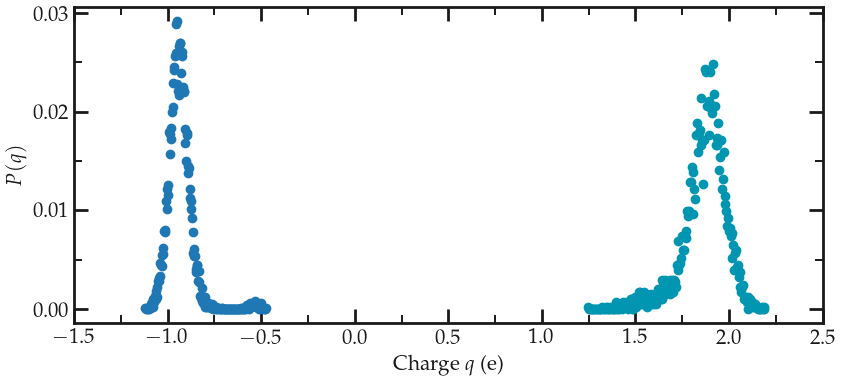
\includegraphics[width=\linewidth]{tutorials/level3/reactive-silicon-dioxide/distribution-charge-light.png}
\end{figure}

Using VMD and coloring the atoms by their charges, one can see that 
the atoms with the extreme-most charges are located at defects in the 
amorphous structure (here at the positions of the dandling oxygen groups):

\begin{figure}
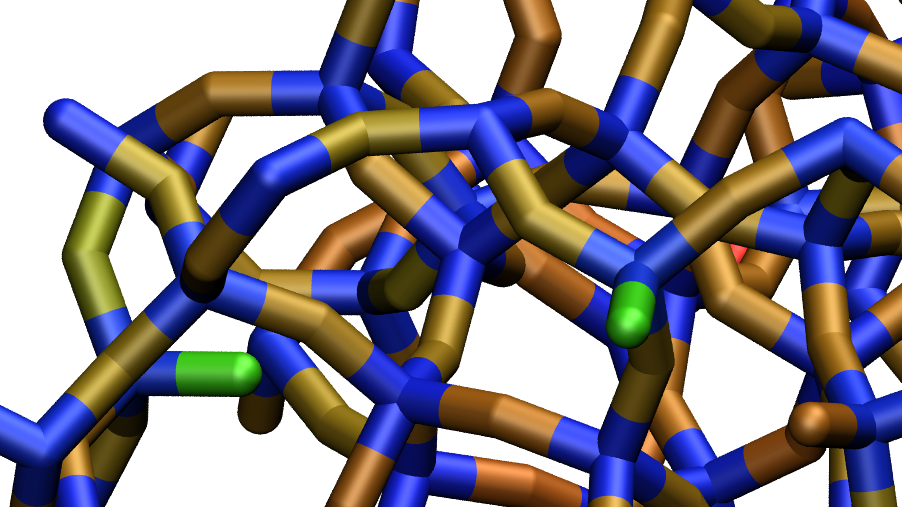
\includegraphics[width=\linewidth]{tutorials/level3/reactive-silicon-dioxide/silicon-light.png}
\end{figure}

Note for VMD user: to color the atoms by their charge, use \textit{Charge} as coloring method in the 
representation windows, and then tune the \textit{Color scale} in the \textit{Color control windows}.

\section{Deform the structure}

\noindent Let us apply a deformation to the structure in order to force some bonds 
to dynamically break and reassemble. 
Next to \textit{RelaxSilica/}, create a folder, call it \textit{Deform/} and create a
file named input.lammps in it. Copy the following lines:

\begin{lcverbatim}
# SiO amorphous silica deformed with reaxff potential
units real
atom_style full
read_data ../RelaxSilica/silica-relaxed.data
mass 1 28.0855 # Si
mass 2 15.999 # O
pair_style reaxff NULL safezone 3.0 mincap 150
pair_coeff * * ../RelaxSilica/reaxCHOFe.ff Si O
fix myqeq all qeq/reaxff 1 0.0 10.0 1.0e-6 reaxff maxiter 400
neighbor 0.5 bin
neigh_modify every 5 delay 0 check yes 
group grpSi type 1
group grpO type 2
variable totqSi equal charge(grpSi)
variable totqO equal charge(grpO)
variable nSi equal count(grpSi)
variable nO equal count(grpO)
variable qSi equal v_totqSi/${nSi}
variable qO equal v_totqO/${nO}
dump dmp all custom 100 dump-deform.lammpstrj id type q x y z
thermo 100
thermo_style custom step temp etotal press vol v_qSi v_qO
fix mynvt all nvt temp 300.0 300.0 100
timestep 0.5 
run 2000
fix mydef all deform 1 x erate 5e-5
run 25000
unfix mydef
undump dmp
dump dmp all custom 100 dump.lammpstrj id type q x y z
run 2000
write_data silica-deformed.data
\end{lcverbatim}

\noindent The main differences with the previous input are
\begin{itemize}
\item the use of fix deform for elongating progressively the box along x,
\item the use of fix NVT instead of NPT (because the box deformation is already ensured by fix deform).
\end{itemize}

After a first run of 25000 steps, a short run of 2000 steps is performed 
in order to extract the final charges of the atoms from an structure that is not 
under deformation.
During the deformation, the charges progressively changes, until the structure eventually
breaks up. After the structure breaks, the charges equilibrates near a new 
average value that differs from the starting charge, which is expected due to the
presence of the new solid/vacuum interface:

\begin{figure}
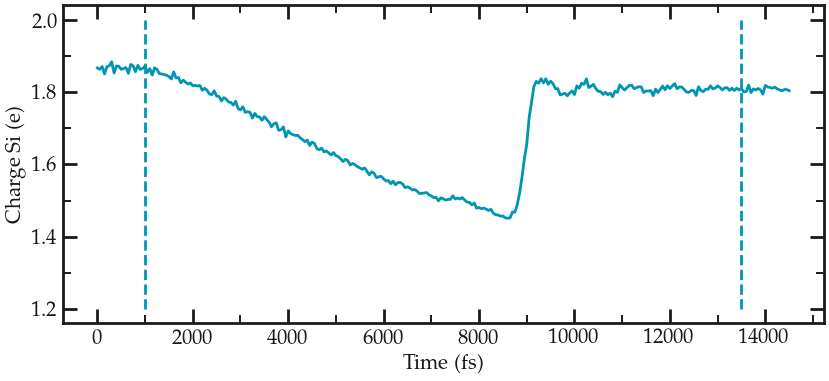
\includegraphics[width=\linewidth]{tutorials/level3/reactive-silicon-dioxide/deformed-charge-light.png}
\end{figure}

At the end of the deformation,  one can visualize the broken material. Notice
the different charge of the atoms located near the interface and compared to the 
atoms located in the bulk of the material:

\begin{figure}
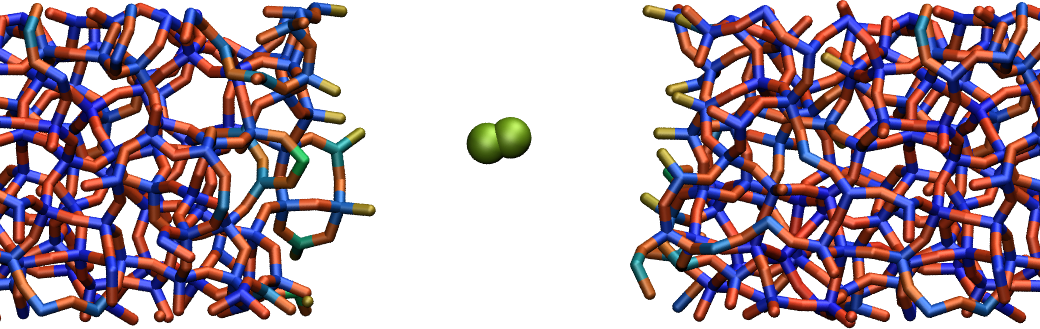
\includegraphics[width=\linewidth]{tutorials/level3/reactive-silicon-dioxide/deformed-light.png}
\end{figure}

One O2 molecule was formed during the process (here appearing in green),
most likely because the rate of deformation was really high.
One can have a look at the final charge distribution:

\begin{figure}
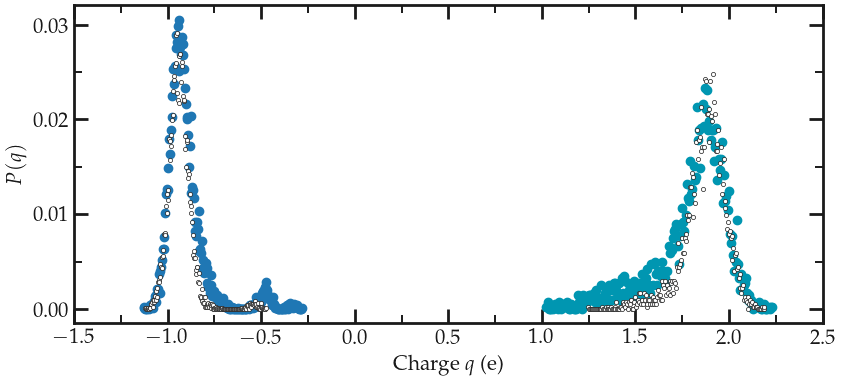
\includegraphics[width=\linewidth]{tutorials/level3/reactive-silicon-dioxide/deformed-distribution-charge-light.png}
\end{figure}

The final charge distribution differs from the previously calculated, as a new peak 
near -0.5e for the oxygen. 

\section{Add O2 molecules}

\noindent Let us add more O2 molecule to our previously equilibrated structure, equilibrate it again, 
and extract the charge density profile along the x axis.
Create a new folder, name it AddOxygen/, and create a new molecule file named O2.mol in it:

\begin{lcverbatim}
# O2 reaxff file
2 atoms
Coords
1 -0.6 0 0
2 0.6 0 0
Types
1        2
2        2   
Charges 
1	0.0
2	0.0
\end{lcverbatim}

\noindent Here the O2 molecule is simply made of 2 oxygen (type 2) atoms that are not 
connected by any bond (because there is no need with reaxff).
Then, create a new input.lammps file, and copy the same first lines as
previously in it: 

\begin{lcverbatim}
units real
atom_style full
read_data ../Deform/silica-deformed.data
mass 1 28.0855 # Si
mass 2 15.999 # O
pair_style reaxff NULL safezone 3.0 mincap 150
pair_coeff * * ../RelaxSilica/reaxCHOFe.ff Si O
fix myqeq all qeq/reaxff 1 0.0 10.0 1.0e-6 reaxff maxiter 400
neighbor 0.5 bin
neigh_modify every 5 delay 0 check yes 
\end{lcverbatim}

\noindent Optionally, let us shift the structure to recenter it in the box. The best value 
for the shift may be different in your case. This step is not necessary, but the
recentered system looks better.

\begin{lcverbatim}
displace_atoms all move -13 0 0 units box
\end{lcverbatim}

\noindent Then, let us import the molecule template O2.mol and create 10 molecules. 
The overlap and maxtry keywords allow us to prevent overlapping
between the atoms:

\begin{lcverbatim}
molecule O2mol O2.mol
create_atoms 0 random 10 456415 NULL mol O2mol 454756 overlap 3.0 maxtry 50
\end{lcverbatim}

\noindent The value of 3 Angstroms for the minimum interatomic overlapping is 
very safe for the present system. Smaller values may lead to molecules being 
too close from each others.
Finally, let us minimize the energy of the system, and run for a relatively long time:

\begin{lcverbatim}
minimize 1.0e-4 1.0e-6 100 1000
reset_timestep 0
group grpSi type 1
group grpO type 2
variable totqSi equal charge(grpSi)
variable totqO equal charge(grpO)
variable nSi equal count(grpSi)
variable nO equal count(grpO)
variable qSi equal v_totqSi/${nSi}
variable qO equal v_totqO/${nO}
dump dmp all custom 1000 dump.lammpstrj id type q x y z
thermo 1000
thermo_style custom step temp etotal press vol v_qSi v_qO
fix mynvt all nvt temp 300.0 300.0 100
timestep 0.5 
run 100000
\end{lcverbatim}

\noindent Run the simulation. You should see additional O2 molecules in the system:

\begin{figure}
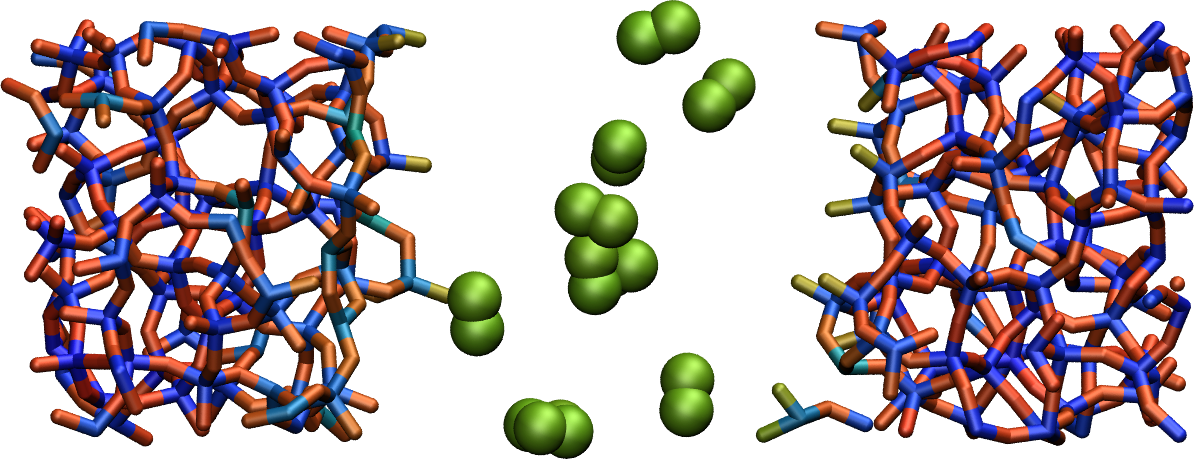
\includegraphics[width=\linewidth]{tutorials/level3/reactive-silicon-dioxide/O2_light.png}
\end{figure}

\section{Exercises}

\noindent \subsection{Decorate dandling oxygens}

Under ambient conditions, dandling oxygen are typically terminated by hydrogen atoms. 
Let us improve the current structure by decorating some of the dandling oxygen with
hydrogen atoms, before relaxing it thanks to reaxff. 
Add hydrogen atoms to the dandling oxygens. Then relax the structure using \textit{reaxff} with LAMMPS.
Hydrogen atoms can be added using \textit{create$\_$atoms} command, \textit{gcmc}, or external \textit{Python} script as I did here:

\begin{figure}
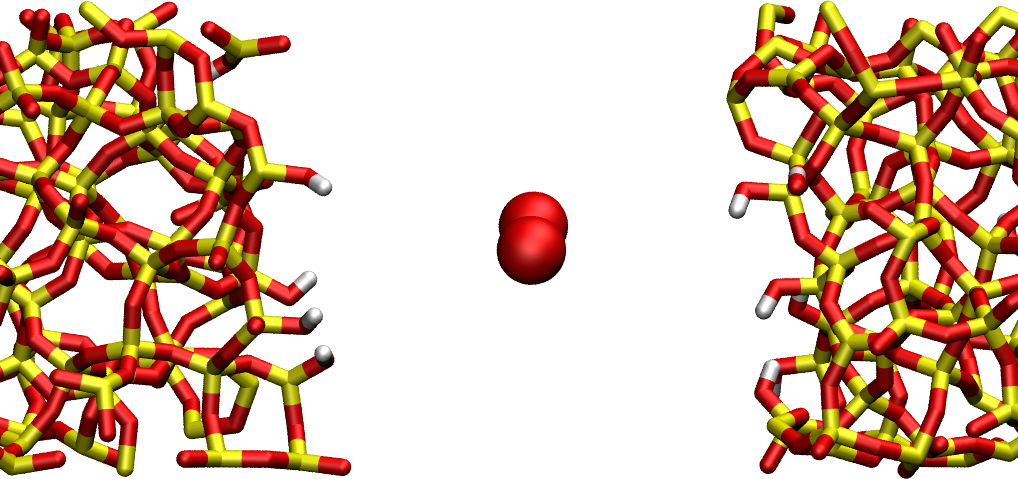
\includegraphics[width=\linewidth]{tutorials/level3/reactive-silicon-dioxide/exercice-light.png}
\end{figure}

\begin{tcolorbox}[colback=mylightblue!5!white,colframe=mylightblue!75!black,title=Hint n°1]
The structure can be imported in MDAnalysis/Python using \textit{u = mda.Universe("silica-deformed.data")}
Then dandling oxygen can be detected by counting the number of neighbor (oxygen with only 
one connected silicon is dandling and should be completed with an hydrogen).
\end{tcolorbox}

\noindent \begin{tcolorbox}[colback=mylightblue!5!white,colframe=mylightblue!75!black,title=Hint n°2]
Once hydrogen have been added, run LAMMPS using:
\begin{lcverbatim}
mass 1 28.0855 # Si
mass 2 15.999 # O
mass 3 1.008 # H
\end{lcverbatim}

\noindent and:
\begin{lcverbatim}
pair_coeff * * reaxCHOFe.ff Si O H
\end{lcverbatim}

\noindent \end{tcolorbox}


\chapter{Water adsorption in silica}

\vspace{-1cm} \noindent \textcolor{graytitle}{\textit{{\Large Dealing with a varying number of molecules}}\vspace{0.5cm} }

\noindent \hspace{-0.45cm}\begin{wrapfigure}{r}{4cm}
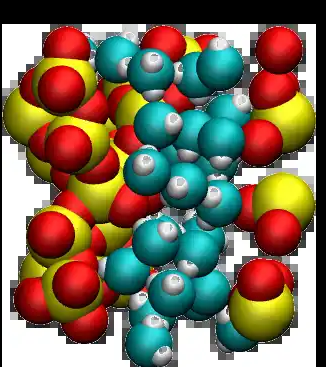
\includegraphics[width=4cm]{tutorials/level3/water-adsorption-in-silica/avatar-light.png}
\end{wrapfigure}

\noindent The objective of this tutorial is to combine molecular
dynamics and grand canonical Monte Carlo simulations to
compute the adsorption of water molecules in a cracked silica material.
This tutorial illustrates the use of the grand canonical
ensemble in molecular simulation, an open ensemble in which the number of 
molecules or atoms is not constant.

\section{Generation of the silica block}

\noindent Let us first generate a block of amorphous silica (SiO2). To do
so, we are going to replicate a building block containing 3
Si and 6 O atoms. 

Create two folders side by side, and name them respectively \textit{Potential/}
and \textit{SilicaBlock/}.
An initial data file for the SiO atoms can be
downloaded by clicking \href{../../../../../inputs/level3/water-adsorption-in-silica/SilicaBlock/SiO.data}{here}.
Save it in \textit{SilicaBlock/}. This data file
contains the coordinates of the 9 atoms, their masses, and
their charges. The fine can be directly read by LAMMPS using the
\textit{read$\_$file} command. Let us replicate these atoms using
LAMMPS, and apply an annealing procedure to obtain a block
of amorphous silica.

\begin{tcolorbox}[colback=mylightblue!5!white,colframe=mylightblue!75!black,title=About annealing procedure]
The annealing procedure consists of adjusting the system temperature in successive steps.
Here, a large initial temperature is chosen to ensure the melting of the SiO2 structure.
Then, several steps are used to progressively cool down the system until it solidifies and forms 
amorphous silica. Depending on the material, different cooling velocities can sometimes
lead to different crystal structure or different degree of defect.
\end{tcolorbox}

\noindent \subsection{Vashishta potential}

Create a new input file named \textit{input.lammps} in the \textit{SilicaBlock/} folder, and copy
the following lines in it:

\begin{lcverbatim}
units metal
boundary p p p
atom_style full
pair_style vashishta
neighbor 1.0 bin
neigh_modify delay 1
\end{lcverbatim}

\noindent The main difference between the previous tutorials is the use of 
the Vashishta pair style. Download the Vashishta potential by
clicking \href{../../../../../inputs/level3/water-adsorption-in-silica/Potential/SiO.1990.vashishta}{here}, and copy it within the \textit{Potential/} folder.

\begin{tcolorbox}[colback=mylightblue!5!white,colframe=mylightblue!75!black,title=About the Vashishta potential]
The \href{https://pubmed.ncbi.nlm.nih.gov/9993674/}{Vashishta}
potential is a bond-angle energy based potential, it
deduces the bonds between atoms from their relative
positions. Therefore, there is no need to provide bond
and angle information as we do with classic force fields
like GROMOS or AMBER.

Note that Vashishta potential requires the use of metal units system. 

Bond-angle energy based potentials
are more computationally heavy than classical force
fields and require the use of a smaller timestep, but
they allow for the modelling of bond formation and
breaking, which is what we need here as we want to create
a crack in the silica.
\end{tcolorbox}

\noindent Let us then import the system made of 9 atoms, replicate it four times in all three
directions of space, thus creating a system with 576 atoms.

\begin{lcverbatim}
read_data SiO.data
replicate 4 4 4
\end{lcverbatim}

\noindent Then, let us specify the pair coefficients by indicating
that the first atom type is Si, and the second is O. Let us also
add a dump command for printing out the positions of the
atoms every 5000 steps:

\begin{lcverbatim}
pair_coeff * * ../Potential/SiO.1990.vashishta Si O
\end{lcverbatim}

\noindent Let us add some commands to help us follow the evolution of the system,
such as its temperature, volume, and potential-energy:

\begin{lcverbatim}
dump dmp all atom 5000 dump.lammpstrj
variable myvol equal vol
variable mylx equal lx
variable myly equal ly
variable mylz equal lz
variable mypot equal pe
fix myat1 all ave/time 10 100 1000 v_mytemp file temperature.dat
fix myat2 all ave/time 10 100 1000 v_myvol v_mylx v_myly v_mylz file dimensions.dat
fix myat3 all ave/time 10 100 1000 v_mypot file potential-energy.dat
thermo 1000
\end{lcverbatim}

\noindent \subsection{Annealing procedure}

Finally, let us create the last part of our script. The
annealing procedure is the following: we first start with a
small phase at 6000 K, then cool down the system to 4000 K
using a pressure of 100 atm. Then we cool down the system
further while also reducing the pressure, then perform a
small equilibration step at the final desired condition, 300
K and 1 atm.
\textit{Disclaimer --} I created this procedure by intuition and
not from proper calibration, do not copy it without
making your own tests if you intend to publish your
results.

\begin{lcverbatim}
velocity all create 6000 4928459 rot yes dist gaussian
fix npt1 all npt temp 6000 6000 0.1 iso 100 100 1
timestep 0.001
run 50000
fix npt1 all npt temp 6000 4000 0.1 aniso 100 100 1
run 50000
fix npt1 all npt temp 4000 300 0.1 aniso 100 1 1
run 200000
fix npt1 all npt temp 300 300 0.1 aniso 1 1 1
run 50000
write_data amorphousSiO.data
\end{lcverbatim}

\noindent \begin{tcolorbox}[colback=mylightblue!5!white,colframe=mylightblue!75!black,title=Anisotropic versus isotropic barostat]
Here, an isotropic barostat is used for the melted phase at 6000 K, and then 
an anisotropic barostat when cooling down the system. With the anisotropic 
barostat, all three directions of space are adjusted independently from one another. Such
anisotropic barostat is usually a better choice for a solid phase, 
when there is no reason for the final solid phase to
have the same dimensions along all 3 axis. For a
liquid or a gas, the isotropic barostat is usually the best choice.
\end{tcolorbox}

\noindent The simulation takes about 15-20 minutes on 4 cpu cores.
Let us check the evolution of the temperature from the \textit{temperature.dat} file.
Apart from an initial spike (may be due to an initial bad configuration, probably harmless here),
the temperature follows well the desired annealing procedure:

\begin{figure}
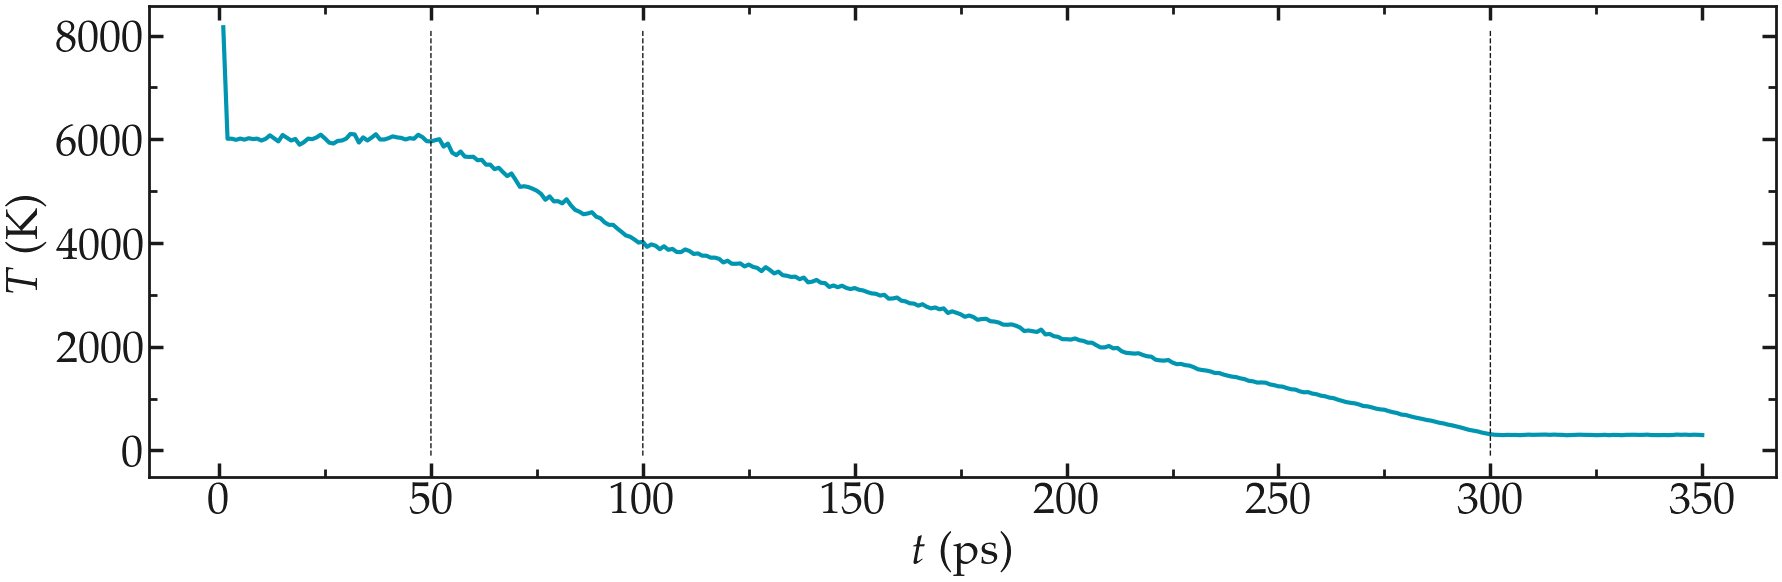
\includegraphics[width=\linewidth]{tutorials/level3/water-adsorption-in-silica/temperature_evolution-light.png}
\end{figure}

Let us also make sure that the box was indeed deformed isotropically during the first 
stage of the simulation, and then anisotropically by plotting lx (blue), ly (orange), and lz:

\begin{figure}
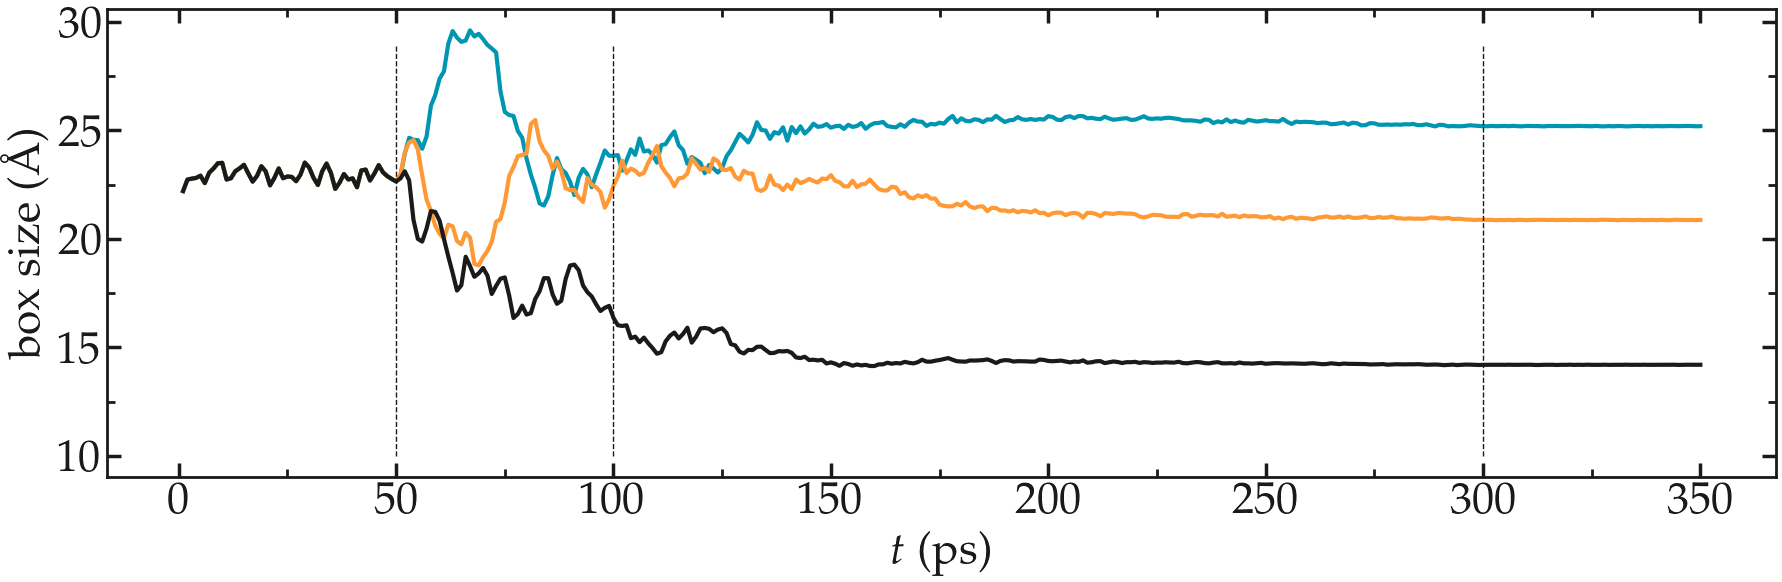
\includegraphics[width=\linewidth]{tutorials/level3/water-adsorption-in-silica/dimensions_evolution-light.png}
\end{figure}

\hspace{-0.45cm}\begin{wrapfigure}{r}{4cm}
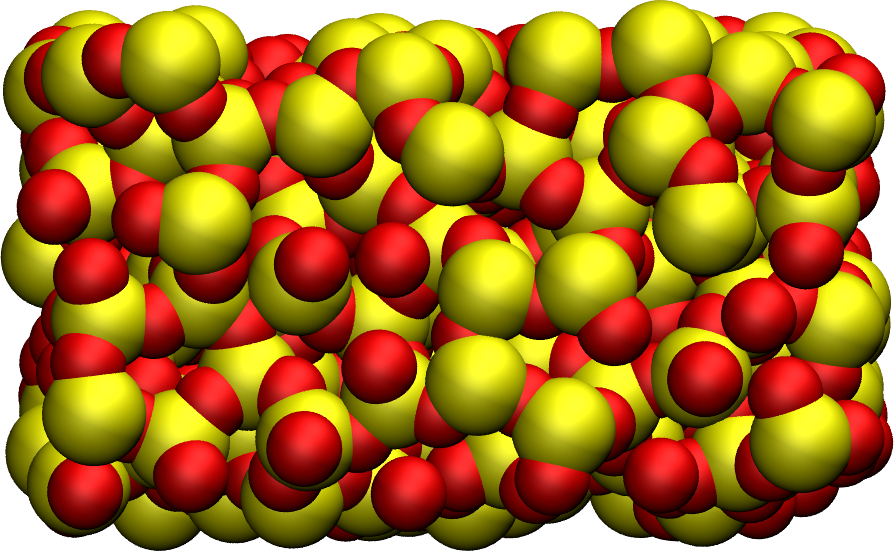
\includegraphics[width=4cm]{tutorials/level3/water-adsorption-in-silica/generated-silica-light.png}
\end{wrapfigure}

\noindent The snapshot on the side shows the final amorphous silica (SiO2).
After running the simulation, the final LAMMPS topology file named
\textit{amorphousSiO.data} will be located in \textit{SilicaBlock/}. Alternatively, if you are only interested in the
next steps of this tutorial, you can download it by clicking
\href{../../../../../inputs/level3/water-adsorption-in-silica/SilicaBlock/amorphousSiO.data}{here}.

\begin{tcolorbox}[colback=mylightblue!5!white,colframe=mylightblue!75!black,title=Tip for research project]
In the case of a research project, the validity of the generated
structure must be tested and compared to reference values, ideally from
experiments. 

For instance, radial distribution functions or Young modulus
can both be compared to experimental values. This is beyond the
scope of this tutorial.
\end{tcolorbox}

\noindent \section{Cracking the silica}

Let us dilate the block of silica to create a
crack. Create a new folder called \textit{Cracking/} next to \textit{SilicaBlock/}, and create a
new input.lammps file starting with:

\begin{lcverbatim}
units metal
boundary p p p
atom_style full
neighbor 1.0 bin
neigh_modify delay 1
read_data ../SilicaBlock/amorphousSiO.data
pair_style vashishta
pair_coeff * * ../Potential/SiO.1990.vashishta Si O
dump dmp all atom 1000 dump.lammpstrj
\end{lcverbatim}

\noindent Then, let us progressively increase the size of the
box in the z direction, thus forcing the silica to deform and crack. To do
so, we are going to make a loop using the jump command. At
every step of the loop, the box dimension over x will
be multiplied by a factor 1.005. Here, we use a NVT
thermostat because we want to impose a deformation of the
volume.

\begin{tcolorbox}[colback=mylightblue!5!white,colframe=mylightblue!75!black,title=NVT vs 2D barostat]
Here, box deformations are applied in the x-direction, while the 
y and z box dimensions are kept constants. 
Another possible choice would be to apply a barostat along the y and z 
direction, allowing the system more freedom to deform. In LAMMPS, this 
can be done by using :
\begin{lcverbatim}
fix npt1 all npt temp 300 300 0.1 y 1 1 1 z 1 1 1
\end{lcverbatim}

\noindent instead of:

\begin{lcverbatim}
fix nvt1 all nvt temp 300 300 0.1
\end{lcverbatim}

\noindent Here, the latter command will be used (see below), but feel free to improvise.
\end{tcolorbox}

\noindent Add the following lines to the input script:

\begin{lcverbatim}
fix nvt1 all nvt temp 300 300 0.1
timestep 0.001
thermo 1000
variable var loop 45
label loop
change_box all x scale 1.005 remap
run 2000
next var
jump input.lammps loop
run 20000
write_data dilatedSiO.data
\end{lcverbatim}

\noindent Use different factor (1.005) or different number of 
loop (45) if you want to generate different defects in the silica.

\hspace{-0.45cm}\begin{wrapfigure}{r}{4cm}
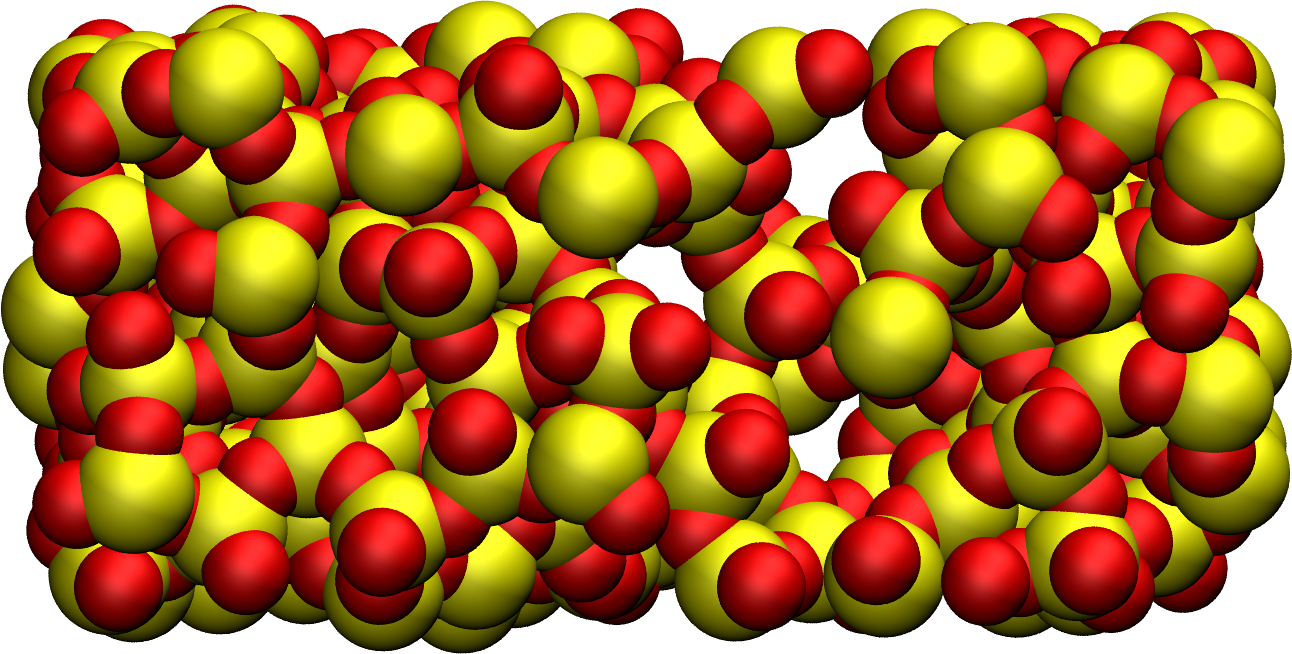
\includegraphics[width=4cm]{tutorials/level3/water-adsorption-in-silica/cracked-light.png}
\end{wrapfigure}

\noindent The snapshot on the side shows the block of silica with holes and deformed bonds.
After the dilatation, a final equilibration step of 20
picoseconds is performed. If you look at the dump file
produced after executing this script, or at \href{https://www.youtube.com/watch?v=8rBqYIcTgno&ab_channel=SimonGravelle}{this video},
you can see the dilatation occurring step-by-step, and the
atoms adjusting progressively to the box size. 

At first, the deformations
are reversible (elastic regime). At some point, bonds
start breaking and dislocations appear (plastic regime). 

Alternatively, you
can download the final state directly by clicking
\href{../../../../../inputs/level3/water-adsorption-in-silica/Cracking/dilatedSiO.data}{here}. The final system, with the crack, resembles:

\begin{tcolorbox}[colback=mylightblue!5!white,colframe=mylightblue!75!black,title=Passivated silica]
In ambient conditions, Some of the surface SiO2 atoms are chemically
passivated by forming covalent bonds with hydrogen (H)
atoms. For the sake of simplicity, we are not going to
add surface hydrogen atoms here. 

An example of procedure allowing for properly inserting hydrogen atoms is given in one 
exercise from this tutorial: :ref:`reactive-silicon-dioxide-label`.
\end{tcolorbox}

\noindent \section{Adding water}

\begin{tcolorbox}[colback=mylightblue!5!white,colframe=mylightblue!75!black,title=About the GCMC method]
In order to add the water molecules to the silica, we are
going to use the Monte Carlo method in the grand canonical
ensemble (GCMC). In short, the system is put into contact
with a virtual reservoir of given chemical potential
$\mu$, and multiple attempts to insert water
molecules at random positions are made. Attempts are
either accepted or rejected based on energy consideration.
If you are interested in learning more about GCMC, I am developing
another website with the goal of delving deeper into the algorithms: \href{https://mdcourse.github.io}{mdcourse.github.io}.
\end{tcolorbox}

\noindent \subsection{Using hydrid potentials}

In a new folder called \textit{Addingwater/}, add this template file
for the water molecule: \href{../../../../../inputs/level3/water-adsorption-in-silica/AddingWater/TIP4P2005.txt}{TIP4P2005.txt}.
Create a new input file, and copy the following lines into it:

\begin{lcverbatim}
units metal
boundary p p p
atom_style full
neighbor 1.0 bin
neigh_modify delay 1
pair_style hybrid/overlay vashishta lj/cut/tip4p/long 3 4 1 1 0.1546 10
kspace_style pppm/tip4p 1.0e-4
bond_style harmonic
angle_style harmonic
\end{lcverbatim}

\noindent There are several differences with the previous input files
used in this tutorial because, from now on, the system will combine water and silica.
Two force fields are combined, Vashishta for
SiO, and lj/cut/tip4p/long for TIP4P water model, which is
done using the hybrid/overlay pair style.
The kspace solver is used to calculate the long
range Coulomb interactions associated with tip4p/long.
Finally, the style for the bonds and angles
of the water molecules are defined (although not important
since its a rigid water model).
Before going further, we also need to make a few change to our data file.
Currently, \textit{dilatedSiO.data} only includes two atom types, but
we need four. Copy the previously generated \textit{dilatedSiO.data}
file within \textit{Addingwater/}. Currently, \textit{dilatedSiO.data} starts with:

\begin{lcverbatim}
LAMMPS data file via write_data, version 2 Aug 2023, timestep = 110000, units = metal
576 atoms
2 atom types
-5.512084438507452 26.09766215010596 xlo xhi
-0.12771230207837192 20.71329001367807 ylo yhi
3.211752393088563 17.373825318513106 zlo zhi
Masses
1 28.0855
2 15.9994
Atoms # full
(...)
\end{lcverbatim}

\noindent Make the following changes to allow for the addition of water
molecules. Modify the file so that it looks like the following 
(with 4 atom types, 1 bond type, 1 angle type, and four masses):

\begin{lcverbatim}
LAMMPS data file via write_data, version 30 Jul 2021, timestep = 90000
576 atoms
4 atom types
1 bond types
1 angle types
2 extra bond per atom
1 extra angle per atom
2 extra special per atom
0.910777522101565 19.67480018949893 xlo xhi
2.1092682236518137 18.476309487947546 ylo yhi
-4.1701120819606885 24.75568979356097 zlo zhi
Masses
1 28.0855
2 15.9994
3 15.9994
4 1.008
Atoms # full
(...)
\end{lcverbatim}

\noindent Doing so, we anticipate that there will be 4 atoms types in
the simulations, with O and H of H2O having indexes 3 and 4,
respectively. There will also be 1 bond type and 1 angle
type. The extra bond, extra angle, and extra special lines
also need to be added for memory allocation. 
We can continue to fill in the
\textit{input.lammps} file, by adding the system definition:

\begin{lcverbatim}
read_data dilatedSiO.data
molecule h2omol TIP4P2005.txt
lattice sc 3
create_atoms 0 box mol h2omol 45585
lattice none 1
group SiO type 1 2
group H2O type 3 4
\end{lcverbatim}

\noindent After reading the data file and defining the h2omol molecule
from the txt file, the \textit{create$\_$atoms} command is used to
include some water molecules in the system on a 
simple cubic lattice. Not adding a molecule before starting the
GCMC steps usually lead to failure. Note that here,
most water molecules are overlapping with the silica. These 
overlapping water molecules will be deleted before 
starting the simulation. 
Then, add the following settings to \textit{Addingwater/input.lammps}:

\begin{lcverbatim}
pair_coeff * * vashishta ../Potential/SiO.1990.vashishta Si O NULL NULL
pair_coeff * * lj/cut/tip4p/long 0 0
pair_coeff 1 3 lj/cut/tip4p/long 0.0057 4.42 # epsilonSi = 0.00403, sigmaSi = 3.69
pair_coeff 2 3 lj/cut/tip4p/long 0.0043 3.12 # epsilonO = 0.0023, sigmaO = 3.091
pair_coeff 3 3 lj/cut/tip4p/long 0.008 3.1589
pair_coeff 4 4 lj/cut/tip4p/long 0.0 0.0
bond_coeff 1 0 0.9572
angle_coeff 1 0 104.52
variable oxygen atom "type==3"
group oxygen dynamic all var oxygen
variable nO equal count(oxygen)
fix myat1 all ave/time 100 10 1000 v_nO file numbermolecule.dat
fix shak H2O shake 1.0e-4 200 0 b 1 a 1 mol h2omol
\end{lcverbatim}

\noindent The force field Vashishta applies only to Si (type 1) and O of SiO2 (type 2),
and not to the O and H of H2O, thanks to the NULL
parameters used for atoms of types 3 and 4. 

Pair coefficients for lj/cut/tip4p/long are
defined between O atoms, as well as between
O(SiO)-O(H2O) and Si(SiO)-O(H2O). Therefore, the fluid-solid 
interactions will be set by Lennard Jones and Coulomb potential. 

The number of oxygen atoms from water molecule (i.e. the number of molecule)
will be printed in the file \textit{numbermolecule.dat}.

The shake algorithm is used to
maintain the shape of the water molecule over time. Some of
these features have been seen in previous tutorials.
Let us delete the overlapping water molecules, and print the 
positions in a dump file:

\begin{lcverbatim}
delete_atoms overlap 2 H2O SiO mol yes
dump dmp all atom 1000 dump.init.lammpstrj
\end{lcverbatim}

\noindent \subsection{GCMC simulation}

Let us make a first equilibration step:

\begin{lcverbatim}
compute_modify thermo_temp dynamic yes
compute ctH2O H2O temp
compute_modify ctH2O dynamic yes
fix mynvt1 H2O nvt temp 300 300 0.1
fix_modify mynvt1 temp ctH2O
compute ctSiO SiO temp
fix mynvt2 SiO nvt temp 300 300 0.1
fix_modify mynvt2 temp ctSiO
timestep 0.001
thermo 1000
run 5000
\end{lcverbatim}

\noindent \begin{tcolorbox}[colback=mylightblue!5!white,colframe=mylightblue!75!black,title=On thermostating groups instead of the entire system]
Two different thermostats are used for SiO and for H2O, respectively. Using 
separate thermostat is usually better when the system contains two separate species, such as one solid and one
liquid. It is particularly important to use two thermostats
here, because the number of water molecules will fluctuate with time.

\end{tcolorbox}

\noindent The \textit{compute$\_$modify} 'dynamic yes' for water is used to specify that the
number of molecules is not constant.
Finally, let us use the fix gcmc and perform the grand
canonical Monte Carlo steps:

\begin{lcverbatim}
variable tfac equal 5.0/3.0
variable xlo equal xlo+0.1
variable xhi equal xhi-0.1
variable ylo equal ylo+0.1
variable yhi equal yhi-0.1
variable zlo equal zlo+0.1
variable zhi equal zhi-0.1
region system block ${xlo} ${xhi} ${ylo} ${yhi} ${zlo} ${zhi} 
fix fgcmc H2O gcmc 100 100 0 0 65899 300 -0.5 0.1 mol h2omol tfac_insert ${tfac} group H2O shake shak full_energy pressure 10000 region system
run 25000
write_data SiOwithwater.data
write_dump all atom dump.lammpstrj
\end{lcverbatim}

\noindent \begin{tcolorbox}[colback=mylightblue!5!white,colframe=mylightblue!75!black,title=Dirty fix]
The region \textit{system} was created to avoid the error "Fix gcmc region extends outside simulation box"
which seems to occur with some LAMMPS version.
\end{tcolorbox}

\noindent The \textit{tfac$\_$insert} option ensures that the correct estimate is
made for the temperature of the inserted water molecules by
taking into account the internal degrees of freedom. Running
this simulation, you should see the number of molecule
increasing progressively. When using the pressure argument,
LAMMPS ignores the value of the chemical potential [here $\mu = -0.5$ eV
which corresponds roughly to ambient conditions (i.e. RH approx 50%).]
The large pressure value of 10000 bars was chosen to ensure that 
some successful insertions of molecules would occur during the 
relatively short duration of the simulation.
When you run the simulation, make sure that some water molecules 
remain in the system after the \textit{delete$\_$atoms} command. You can control 
that either using the log file, or using the \textit{numbermolecule.dat} data file.
Depending on your LAMMPS version, you may have to run LAMMPS
on a single cpu core, due to some restrictions of the fix gcmc.
You can see, by looking at the log file, that 280 molecules
were added by the \textit{create$\_$atoms} command (the exact number may differ):

\begin{lcverbatim}
Created 840 atoms
\end{lcverbatim}

\noindent You can also see that 258 molecules where immediately deleted,
leaving 24 water molecules (the exact number may differ):

\begin{lcverbatim}
Deleted 774 atoms, new total = 642
Deleted 516 bonds, new total = 44
Deleted 258 angles, new total = 22
\end{lcverbatim}

\noindent After just a few GCMC steps, you should see that the number of molecules increases with time.
When the crack is fully filled, the number of molecule reaches a plateau:

\begin{figure}
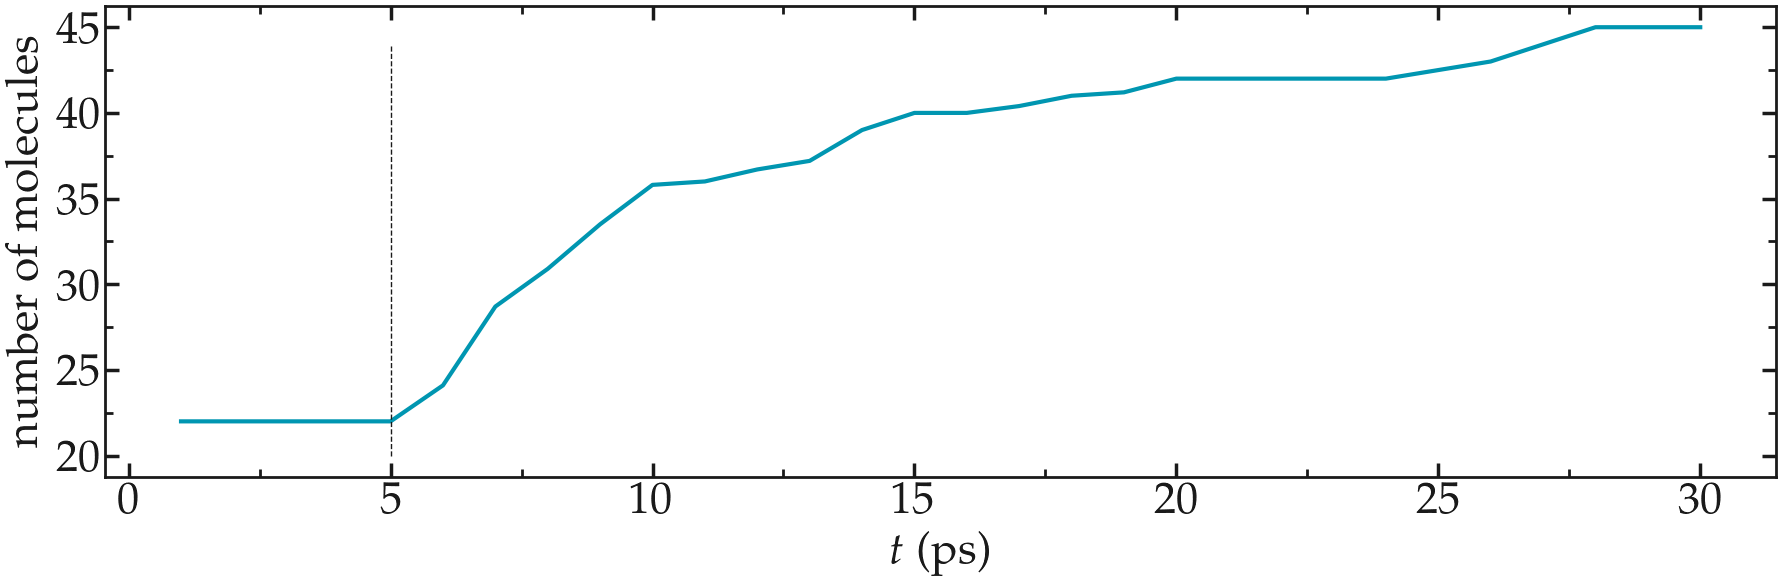
\includegraphics[width=\linewidth]{tutorials/level3/water-adsorption-in-silica/number_evolution-light.png}
\end{figure}

Note that the final number of molecules depends on the imposed pressure, 
temperature, and on the interaction between water and silica (its hydrophilicity). 

\hspace{-0.45cm}\begin{wrapfigure}{r}{4cm}
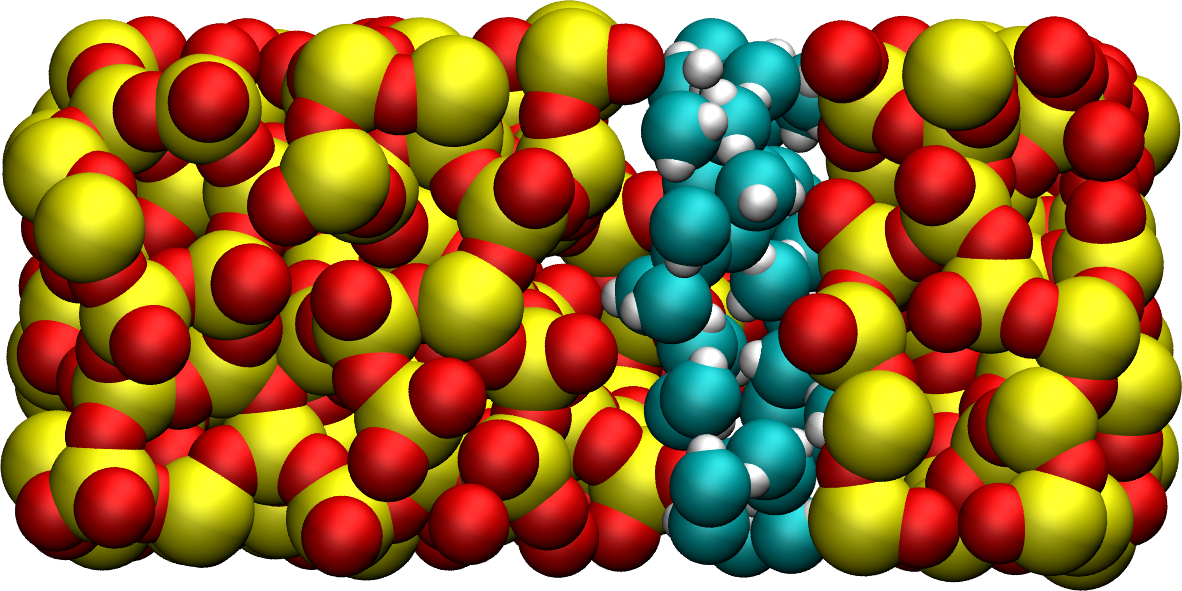
\includegraphics[width=4cm]{tutorials/level3/water-adsorption-in-silica/solvated-light.png}
\end{wrapfigure}

\noindent The figure on the side shows a snapshot of the final state, with the oxygen of the
water molecules represented in cyan.
Note that gcmc simulations of such dense phases are usually slow to converge due to the
very low probability of successfully inserting a molecule. Here, the short simulation 
duration was made possible by the use of a huge pressure.

\begin{tcolorbox}[colback=mylightblue!5!white,colframe=mylightblue!75!black,title=Vizualising varying number of molecules]
By default, VMD fails to properly render systems with varying number of atoms,
but Ovito does it well.
\end{tcolorbox}

\noindent \section{Exercises}

.. include:: ../../contact/requestsolution.rst

\subsection{Apply GCMC to water in ZIF-8 }

\noindent \hspace{-0.45cm}\begin{wrapfigure}{r}{4cm}
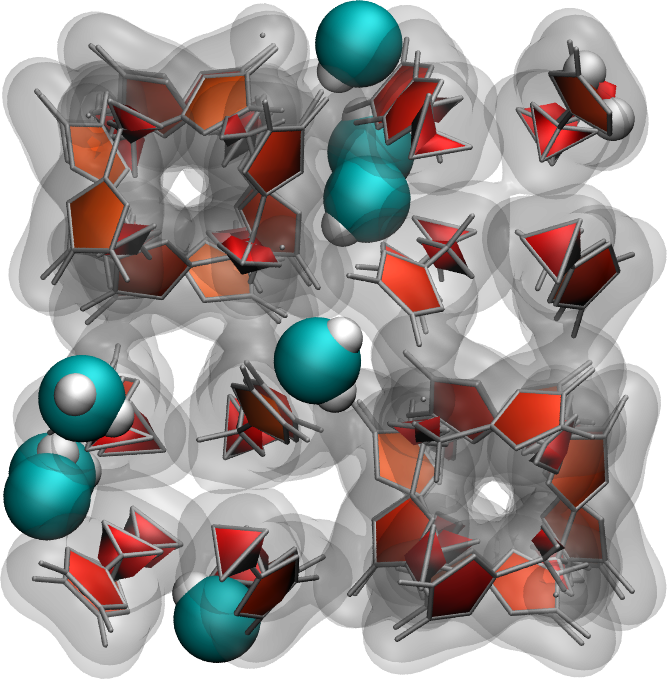
\includegraphics[width=4cm]{tutorials/level3/water-adsorption-in-silica/zif8-light.png}
\end{wrapfigure}

\noindent Use the same protocole as the one implemented in this tutorial to add water
molecules to a Zif-8 nanoporous material. A snapshot of the system with a 
few water molecules is presented on the right.
Download the initial Zif-8 \href{../../../../../inputs/level3/water-adsorption-in-silica/Exercises/Zif-8/zif-8.data}{structure}, the \href{../../../../../inputs/level3/water-adsorption-in-silica/Exercises/Zif-8/parm.lammps}{parameters} file, and this
new \href{../../../../../inputs/level3/water-adsorption-in-silica/Exercises/Zif-8/water.mol}{water template}. The ZIF-8 structure is made of 7 atom types (C1, C2, C3, H2, H3, N, Zn), connected
by bonds, angles, dihedrals, and impropers. It uses the same \textit{pair$\_$style} as water,
so there is no need to use the \textit{hybrid} functionality (see the hints below).
Note that, here, water occupies the atom types 1 and 2, instead of 3 and 4 in the case of SiO2.

\begin{tcolorbox}[colback=mylightblue!5!white,colframe=mylightblue!75!black,title=Hints]
Use the following parameters to start your LAMMPS input file.
\begin{lcverbatim}
units real
atom_style full
boundary p p p
bond_style harmonic
angle_style harmonic
dihedral_style hybrid charmm opls
improper_style harmonic
pair_style lj/cut/tip4p/long 1 2 1 1 0.105 14.0
kspace_style pppm/tip4p 1.0e-5
special_bonds lj 0.0 0.0 0.5 coul 0.0 0.0 0.833
\end{lcverbatim}

\noindent \end{tcolorbox}


\chapter{Free energy calculation}
\label{umbrella-sampling-label}

\vspace{-1cm} \noindent \textcolor{graytitle}{\textit{{\Large Simple sampling of a free energy barrier using umbrella sampling}}\vspace{0.5cm} }

\noindent \hspace{-0.45cm}\begin{wrapfigure}{r}{4cm}
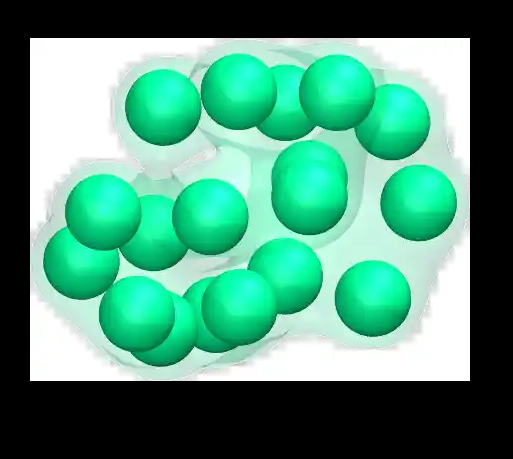
\includegraphics[width=4cm]{tutorials/level3/free-energy-calculation/avatar_light.png}
\end{wrapfigure}

\noindent The objective of this tutorial is to measure the free
energy profile across a barrier potential using two methods;
free sampling and umbrella sampling.

For the sake of simplicity and in order to reduce the computation time, the
barrier potential will be imposed artificially to the atoms.
The procedure is valid for more complex
systems, and can be adapted to many other situations, for instance 
for measuring adsorption barrier near a wall, or for calculating translocation
barrier through a membrane.

\section{Method 1: Free sampling}

\noindent The most direct way to calculate a free energy profile is to extract
the partition function from a classic (unbiased) molecular
dynamics simulation, and then to estimate the Gibbs free
energy using 

where $\Delta G$ is the free energy difference, R the
gas constant, T the temperature, p the
pressure, and $p_0$ the reference pressure.
As an illustration, let us apply this method to an
extremely simple configuration that consists in a few
particles diffusing in a box in presence of a
position-dependent repealing force that makes the centre
of the box a relatively unfavourable area to explore.

\subsection{Basic LAMMPS parameters}

\noindent Create a folder named \textit{FreeSampling/}, and create an input script
named \textit{input.lammps} in it. Copy the following lines:

\begin{lcverbatim}
# define some variables
variable sigma equal 3.405 # Angstrom
variable epsilon equal 0.238 # Kcal/mol
variable U0 equal 1.5*${epsilon} # Kcal/mol
variable dlt equal 1.0 # Angstrom
variable x0 equal 10.0  # Angstrom
# initialise the simulation
units real
atom_style atomic
pair_style lj/cut 3.822 # 2^(1/6) * 3.405 WCA potential
pair_modify shift yes
boundary p p p
\end{lcverbatim}

\noindent Here, we start by defining variables for the Lennard-Jones
interaction $\sigma$ and $\epsilon$ and for
the repulsive potential $U (x)$: $U_0$, $\delta$, and $x_0$, 
see the analytical expression below.
The system of unit 'real' (for which energy is in kcal/mol, distance in Ångstrom,
time in femtosecond) has been chosen for practical reason,
as the WHAM algorithm we are going to use in the second
part of the tutorial automatically assumes the energy to
be in kcal/mol. Atoms will interact through a
Lennard-Jones potential with a cut-off equal to 
$\sigma \times 2 ^ {1/6}$ (i.e. a WCA repulsive
potential). The potential is shifted to be equal to 0 at
the cut-off using the \textit{pair$\_$modify}.

\subsection{System creation and settings}

\noindent Let us define the simulation block and randomly add atoms:

\begin{lcverbatim}
# define the system
region myreg block -25 25 -5 5 -25 25
create_box 1 myreg
create_atoms 1 random 60 341341 myreg overlap 1.0 maxtry 50
# settings
mass * 39.95
pair_coeff * * ${epsilon} ${sigma}
neigh_modify every 1 delay 4 check yes
\end{lcverbatim}

\noindent Here I am using the argon's values of the Lennard-Jones parameters $\sigma$ and
$\epsilon$, as well as the mass $m = 39.95$
grams/mole. 

In the previous subsection, the variables $U_0$, $\delta$, and
$x_0$ were defined. They are used to create the repulsive potential
restricting the atoms to explore the center of the box: 

$$U(x) = U_0 \left[ \arctan \left( \dfrac{x+x_0}{\delta} \right) - \arctan \left(\dfrac{x-x_0}{\delta} \right) \right]. $$
From the derivative of the
potential with respect to $x$, we obtain the expression
for the force that will be imposed to the atoms:

$$F(x)= \dfrac{U_0}{\delta} \left[ \dfrac{1}{(x-x_0)^2/\delta^2+1} - \dfrac{1}{(x+x_0)^2/\delta^2+1} \right].$$
The potential and force along the $x$
axis resemble:

\begin{figure}
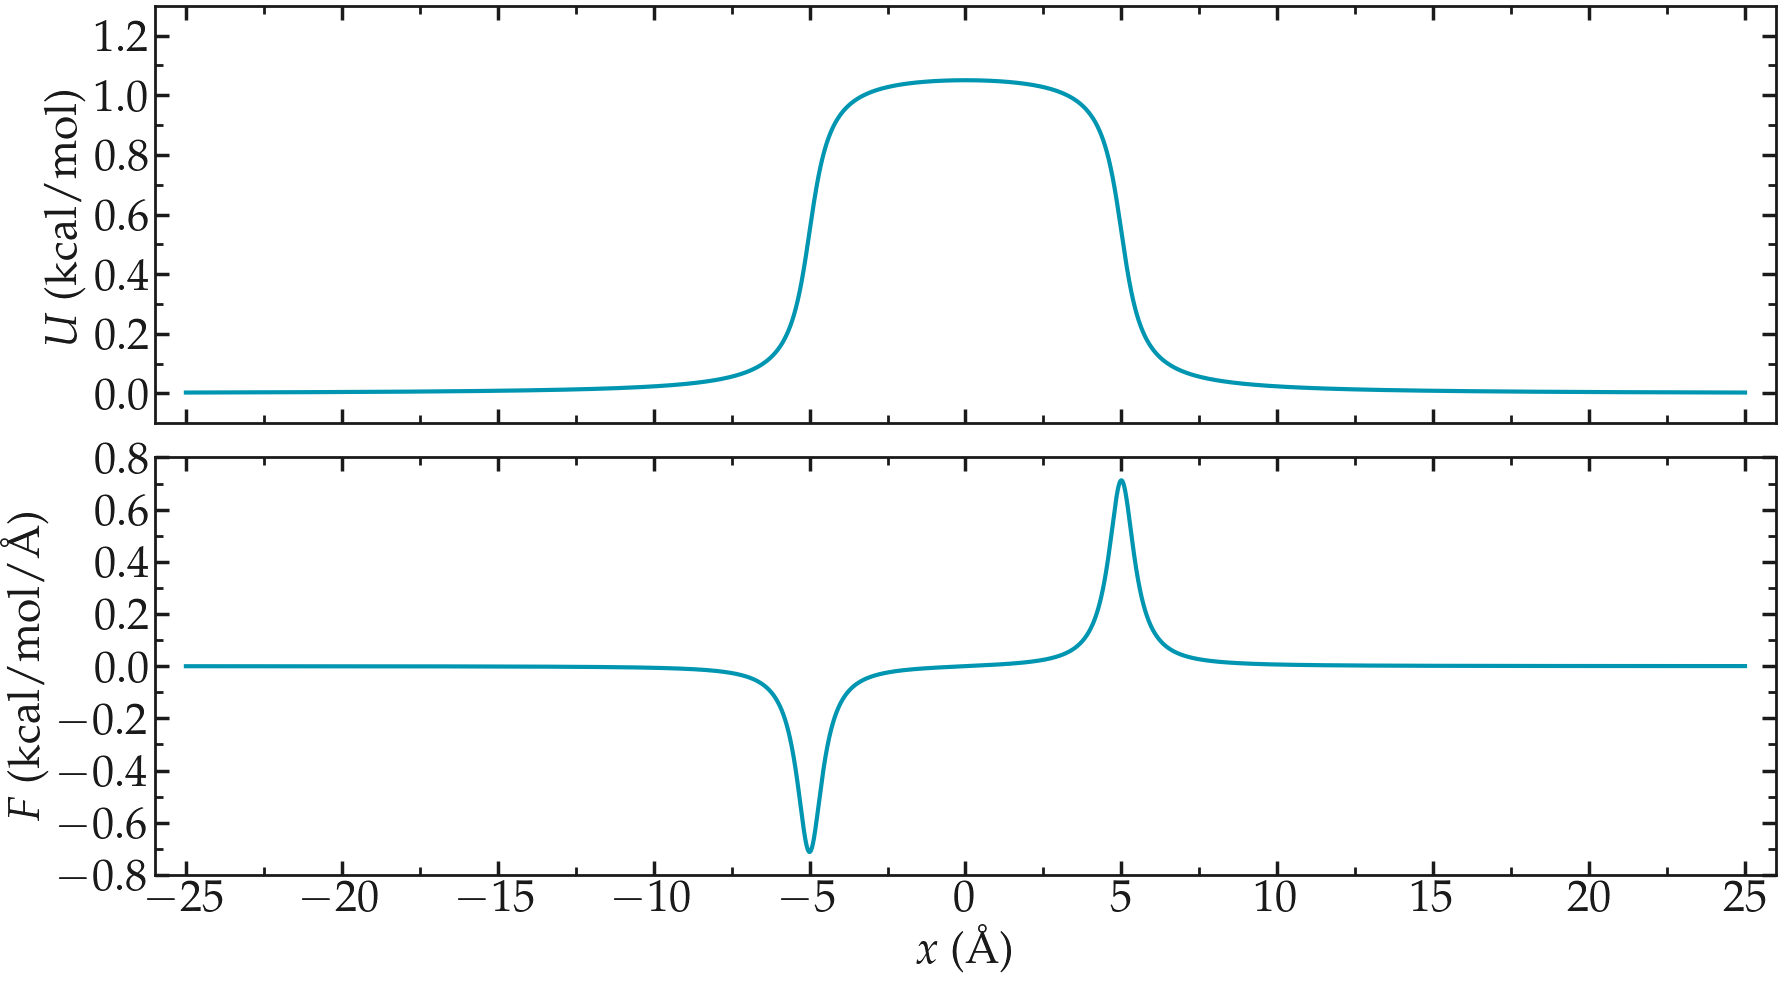
\includegraphics[width=\linewidth]{tutorials/level3/free-energy-calculation/potential-light.png}
\end{figure}

Let us apply energy minimization to the system, and then impose
the force \\(F(x)\\) to all of the atoms in the simulation using the 'addforce' command:

\begin{lcverbatim}
# --------------------- Run
minimize 1e-4 1e-6 100 1000
reset_timestep 0
variable U atom ${U0}*atan((x+${x0})/${dlt})-${U0}*atan((x-${x0})/${dlt})
variable F atom ${U0}/((x-${x0})^2/${dlt}^2+1)/${dlt}-${U0}/((x+${x0})^2/${dlt}^2+1)/${dlt}
fix myadf all addforce v_F 0.0 0.0 energy v_U
\end{lcverbatim}

\noindent Finally, let us combine the fix nve with a Langevin
thermostat to run a molecular dynamics simulation. With
these two commands, the MD simulation is effectively in the
NVT ensemble: constant number of atoms $N$, constant
volume $V$, and constant temperature $T$. Let us
perform an equilibration of 500000 steps in total,
using a timestep of 2 ps (i.e. a total duration of 1
nanoseconds). To make sure that 1 ns is long enough, let us
record the evolution of the number of atoms in the central
(energetically unfavorable) region called \textit{mymes}:

\begin{lcverbatim}
fix mynve all nve
fix mylgv all langevin 119.8 119.8 50 1530917
region mymes block -${x0} ${x0} INF INF INF INF 
variable n_center equal count(all,mymes)
fix myat all ave/time 10 50 500 v_n_center file density_evolution.dat
timestep 2.0
thermo 10000
run 500000
\end{lcverbatim}

\noindent \subsection{Run and data acquisition}

Finally, let us record the density profile of the atoms
along the $x$ axis using the 'ave/chunk' command. A
total of ten density profiles will be printed. Step counts are
reset to 0 to synchronize with the output times of
density/number, and the fix 'myat' is canceled (it has to be
canceled before a reset time).

\begin{lcverbatim}
unfix myat
reset_timestep 0
compute cc1 all chunk/atom bin/1d x 0.0 1.0
fix myac all ave/chunk 10 400000 4000000 cc1 density/number file density_profile_8ns.dat
dump mydmp all atom 200000 dump.lammpstrj
thermo 100000
run 4000000
\end{lcverbatim}

\noindent This simulation with a duration of 8 ns needs a few
minutes to complete. Feel free to increase the 
duration of the run for smoother results.

You can visualize the dump file using VMD:

\begin{figure}
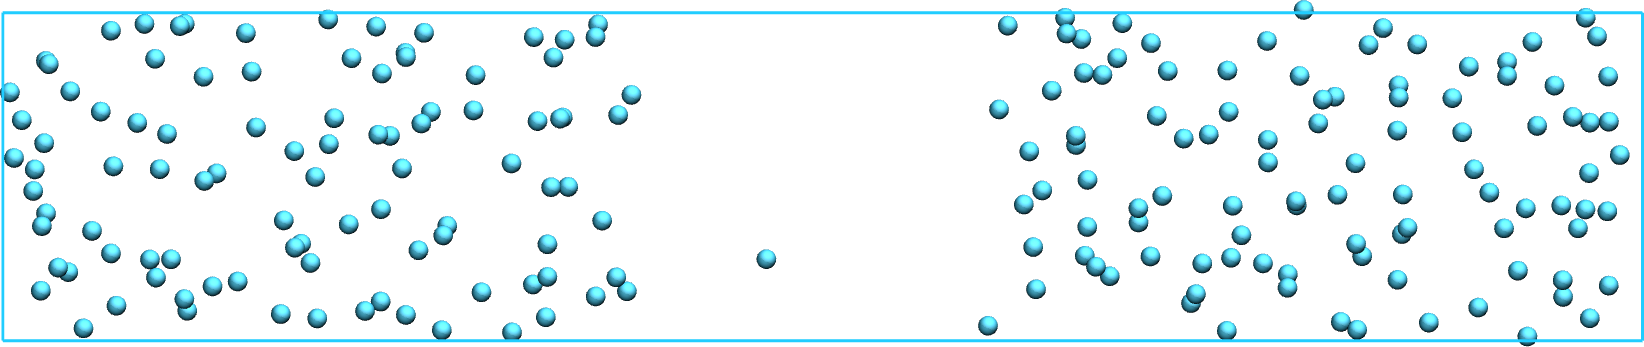
\includegraphics[width=\linewidth]{tutorials/level3/free-energy-calculation/system-light.png}
\end{figure}

\subsection{Data analysis}

\noindent First, let us make sure that the equilibration duration of 1
ns is long enough by looking at the \textit{density$\_$evolution.dat} file:

\begin{figure}
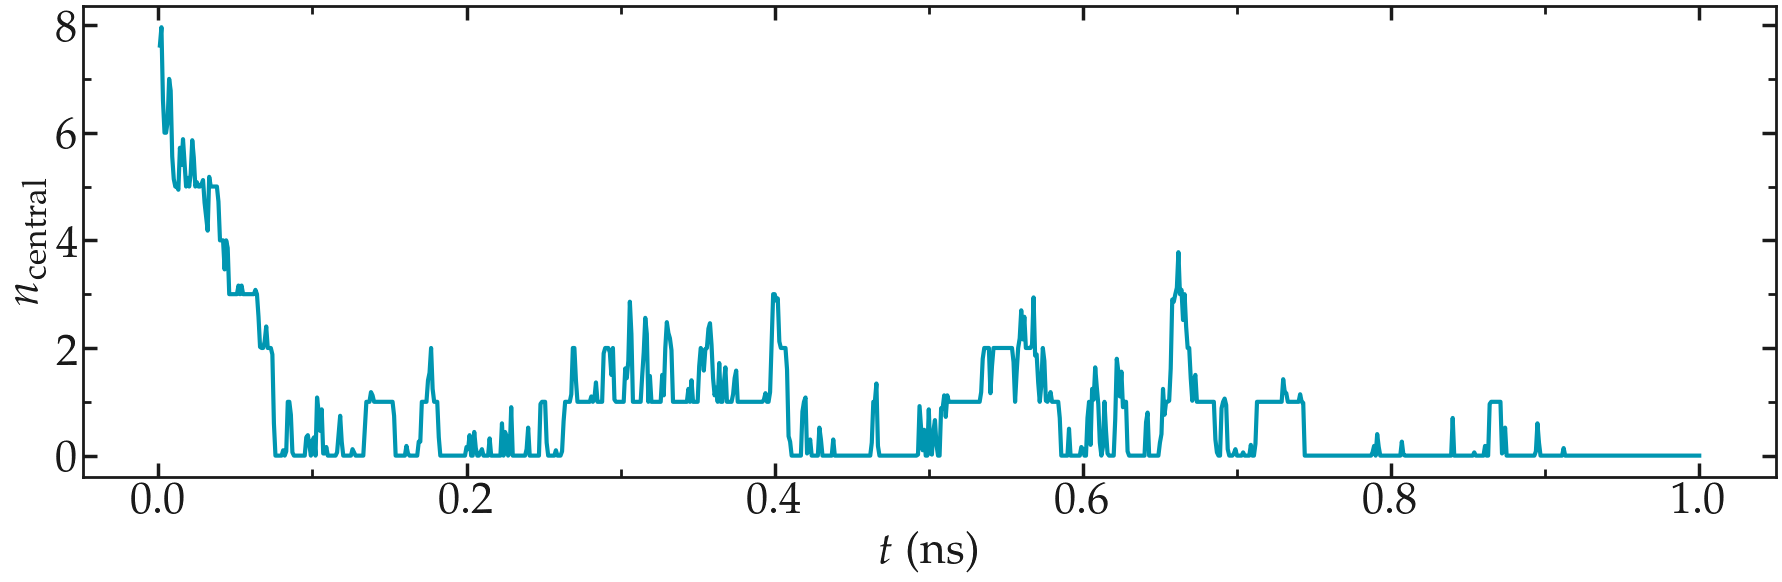
\includegraphics[width=\linewidth]{tutorials/level3/free-energy-calculation/density_evolution-light.png}
\end{figure}

Here, we can clearly see that the number of atoms in the
central region, $n_\mathrm{central}$, evolves to its equilibrium value
after about 0.1 ns.

Let us also plot the equilibrium density profile $\rho$:

\begin{figure}
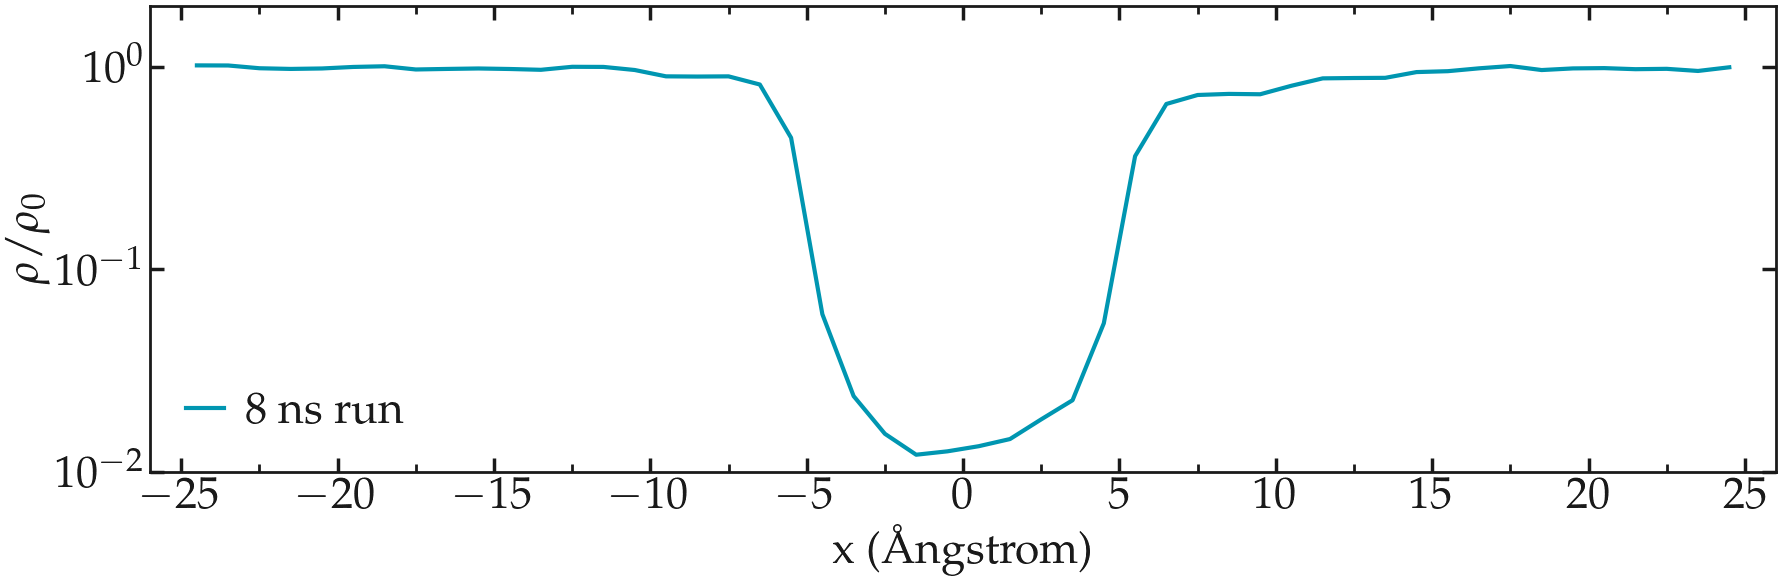
\includegraphics[width=\linewidth]{tutorials/level3/free-energy-calculation/density_profile-light.png}
\end{figure}

Then, let us plot $-R T \ln(\rho/\rho_\mathrm{bulk})$ and compare it
with the imposed (reference) potential $U$:

\begin{figure}
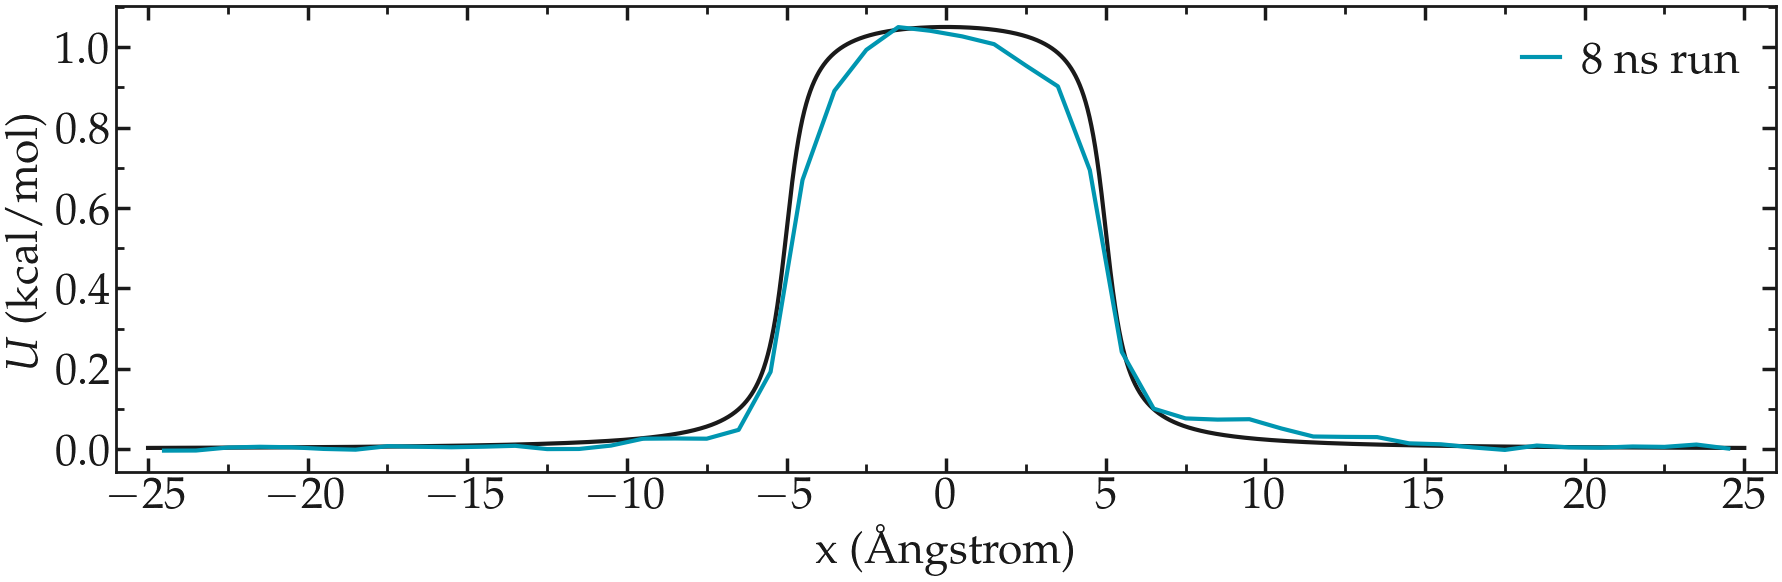
\includegraphics[width=\linewidth]{tutorials/level3/free-energy-calculation/freesampling-potential-light.png}
\end{figure}

The agreement with the expected energy profile is reasonable,
despite some noise in the central part. 

\subsection{The limits of free sampling}

\noindent If we increase the value of $U_0$, the average number of
atoms in the central region will decrease, making it
difficult to obtain a good resolution for the free energy
profile.
In that case, it is better to use the umbrella sampling method
to extract free energy profiles, see the next section.

\section{Method 2: Umbrella sampling}

\noindent Umbrella sampling is a biased molecular dynamics method,
i.e. a method in which additional forces are added to the
atoms in order to make the unfavourable states more likely
to occur.

Keeping the present configuration, we are going to force one of the atom to
explore the central region of the box. To do so, we
are going to add a potential $V$ to one
of the particle, and force it to move along the axe $x$.
The chosen path is called the axe of reaction. The final
simulation will be analyzed using the weighted histogram
analysis method (WHAM), which allows to remove the effect of
the bias and eventually deduce the unbiased free energy profile.

\subsection{LAMMPS input script}

\noindent Create a new folder called \textit{BiasedSampling/}, create a new input file 
named \textit{input.lammps} in it, and copy the following lines:

\begin{lcverbatim}
# define a bunch of variables
variable sigma equal 3.405 # Angstrom
variable epsilon equal 0.238 # Kcal/mol
variable U0 equal 10*${epsilon} # Kcal/mol
variable dlt equal 0.5 # Angstrom
variable x0 equal 5.0  # Angstrom
variable k equal 1.5 # Kcal/mol/Angstrom^2
# initialise the simulation
units real
atom_style atomic
pair_style lj/cut 3.822 # 2^(1/6) * 3.405 WCA potential
pair_modify shift yes
boundary p p p
# define the system
region myreg block -25 25 -5 5 -25 25
create_box 2 myreg
create_atoms 2 single 0 0 0
create_atoms 1 random 5 341341 myreg overlap 1.0 maxtry 50
# settings
mass * 39.948
pair_coeff * * ${epsilon} ${sigma}
neigh_modify every 1 delay 4 check yes
group topull type 2
# run
variable U atom ${U0}*atan((x+${x0})/${dlt})-${U0}*atan((x-${x0})/${dlt})
variable F atom ${U0}/((x-${x0})^2/${dlt}^2+1)/${dlt}-${U0}/((x+${x0})^2/${dlt}^2+1)/${dlt}
fix pot all addforce v_F 0.0 0.0 energy v_U
fix mynve all nve
fix mylgv all langevin 119.8 119.8 50 1530917
timestep 2.0
thermo 100000
run 500000
reset_timestep 0
dump mydmp all atom 1000000 dump.lammpstrj
\end{lcverbatim}

\noindent So far, this code resembles the one of Method 1,
except for the additional particle of type 2. This
particle is identical to the particles of type 1 (same
mass and Lennard-Jones parameters), but will be exposed to the
biasing potential.
The value of the potential $U_0$ was chosen to be much larger than in part 1, 
just to proof that umbrella sampling can easily deal with huge potential value,
while free sampling couldn't.
Let us create a loop with 50 steps, and move progressively
the centre of the bias potential by increment of 0.1 nm:

\begin{lcverbatim}
variable a loop 50
label loop
variable xdes equal ${a}-25
variable xave equal xcm(topull,x)
fix mytth topull spring tether ${k} ${xdes} 0 0 0
run 200000
fix myat1 all ave/time 10 10 100 v_xave v_xdes file data-k1.5/position.${a}.dat
run 1000000
unfix myat1
next a
jump SELF loop
\end{lcverbatim}

\noindent A folder named \textit{data-k1.5/} needs to be created within \textit{BiasedSampling/}.
The spring command serves to impose the
additional harmonic potential with spring constant $k$.
Note that the value of $k$ should be chosen with care,
if its too small, the particle wont follow the biasing potential
center, if its too large, there will be no overlapping between the 
different windows.
The centre of the harmonic potential $x_\text{des}$
successively takes values from -25 to 25. For each value of
$x_\text{des}$, an equilibration step of 0.4 ns is
performed, followed by a step of 2 ns during which the
position along $x$ of the particle is saved in data
files (one data file per value of $x_\text{des}$). You
can always increase the duration of the runs for better samplings.

\subsection{WHAM algorithm}

\noindent In order to generate the free energy profile from the density distribution, we are going to use
the WHAM algorithm. You can download it from \href{http://membrane.urmc.rochester.edu/?page_id=126}{Alan Grossfield} website, or alternatively use 
the \href{../../../../../inputs/level3/free-energy-calculation/BiasedSampling/wham-release-2.0.11.tgz}{version 2.0.11} I have downloaded, or try your luck with the version 
i did precompile; \href{../../../../../inputs/level3/free-energy-calculation/BiasedSampling/wham}{precompiled wham}. After extraction, it can be compiled by simply running:

\begin{lcverbatim}
cd wham
make clean
make
\end{lcverbatim}

\noindent The compilation creates an executable called \textit{wham} that you can 
copy in the \textit{BiasedSampling/} folder.
In order to apply the WHAM algorithm to our simulation, we
first need to create a metadata file. This file simply
contains 

\begin{itemize}
\item the paths to all the data files,
\item the value of $x_\text{des}$,
\item and the values of $k$.
\end{itemize}

To generate the \textit{metadata.txt} file, you can run this Python script
from the \textit{BiasedSampling/} folder:

\begin{lcverbatim}
import os
k=1.5 # set the value of  k in kCal/mol
folder='data-k1.5/'
f = open("metadata.dat", "w")
for n in range(-50,50):
f.close()
\end{lcverbatim}

\noindent The generated file named \textit{metadata.dat} looks like that:

\begin{lcverbatim}
./data-k1.5/position.1.dat -24 1.5
./data-k1.5/position.2.dat -23 1.5
./data-k1.5/position.3.dat -22 1.5
(...)
./data-k1.5/position.48.dat 23 1.5
./data-k1.5/position.49.dat 24 1.5
./data-k1.5/position.50.dat 25 1.5
\end{lcverbatim}

\noindent Alternatively, you can download my \href{../../../../../inputs/level3/free-energy-calculation/BiasedSampling/metadata.dat}{metadata.dat} file.
Then, simply run the following command in the terminal:

\begin{lcverbatim}
./wham -25 25 50 1e-8 119.8 0 metadata.dat PMF.dat
\end{lcverbatim}

\noindent where -25 and 25 are the boundaries, 50 the number of bins,
1e-8 the tolerance, and 119.8 the temperature. A file named
PMF.dat has been created, and contains the free energy
profile in Kcal/mol.

We can compare the result of the PMF with the imposed potential $U$:

\begin{figure}
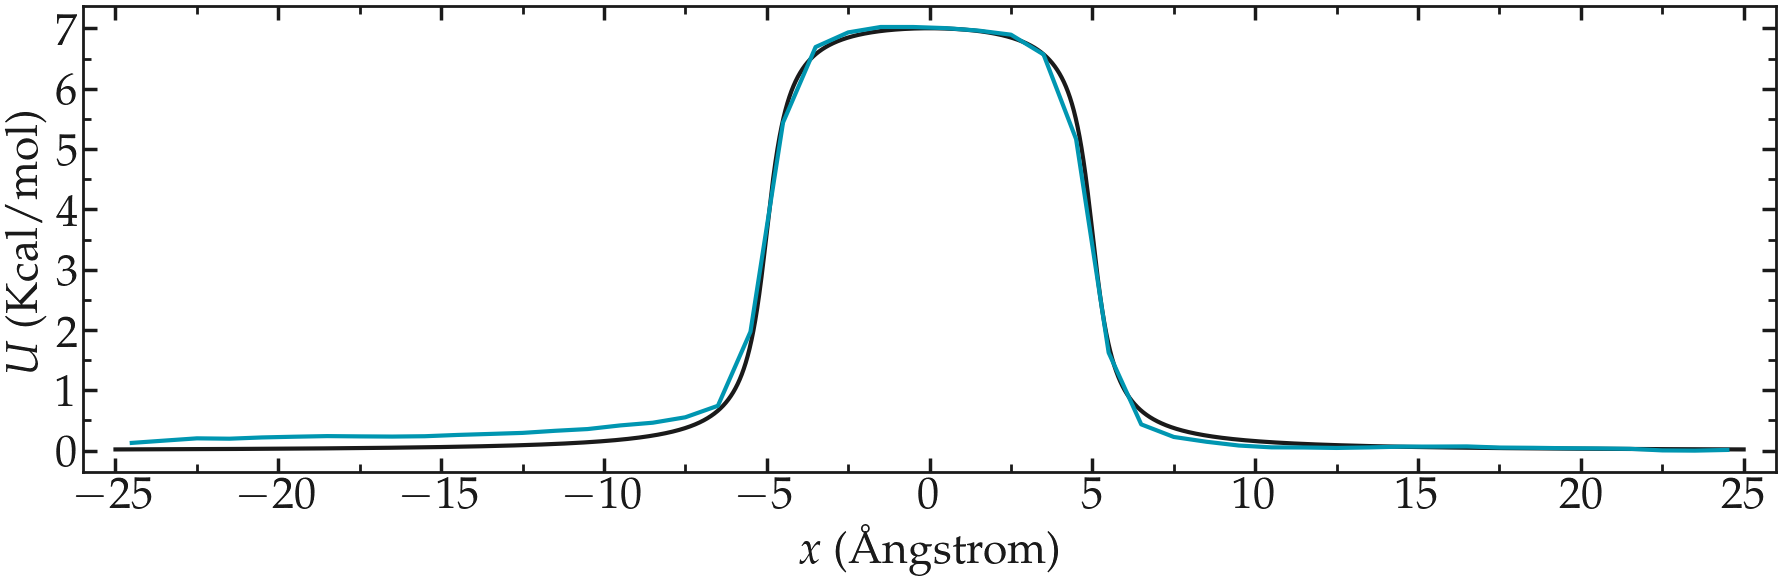
\includegraphics[width=\linewidth]{tutorials/level3/free-energy-calculation/freeenergy-light.png}
\end{figure}

We can see that the agreement is quite good despite the very short calculation time
and the very high value for the energy barrier. 

\subsection{Side note: on the choice of k}

\noindent As already stated, one difficult part of umbrella sampling is to choose the value of $k$.
Ideally, you want the biasing potential to be strong enough to force
the chosen atom to move along the axis, and you also want the
fluctuations of the atom position to be large enough to
have some overlap in the density probability of two
neighbor positions, like we have here with $k = 1.5$:

\begin{figure}
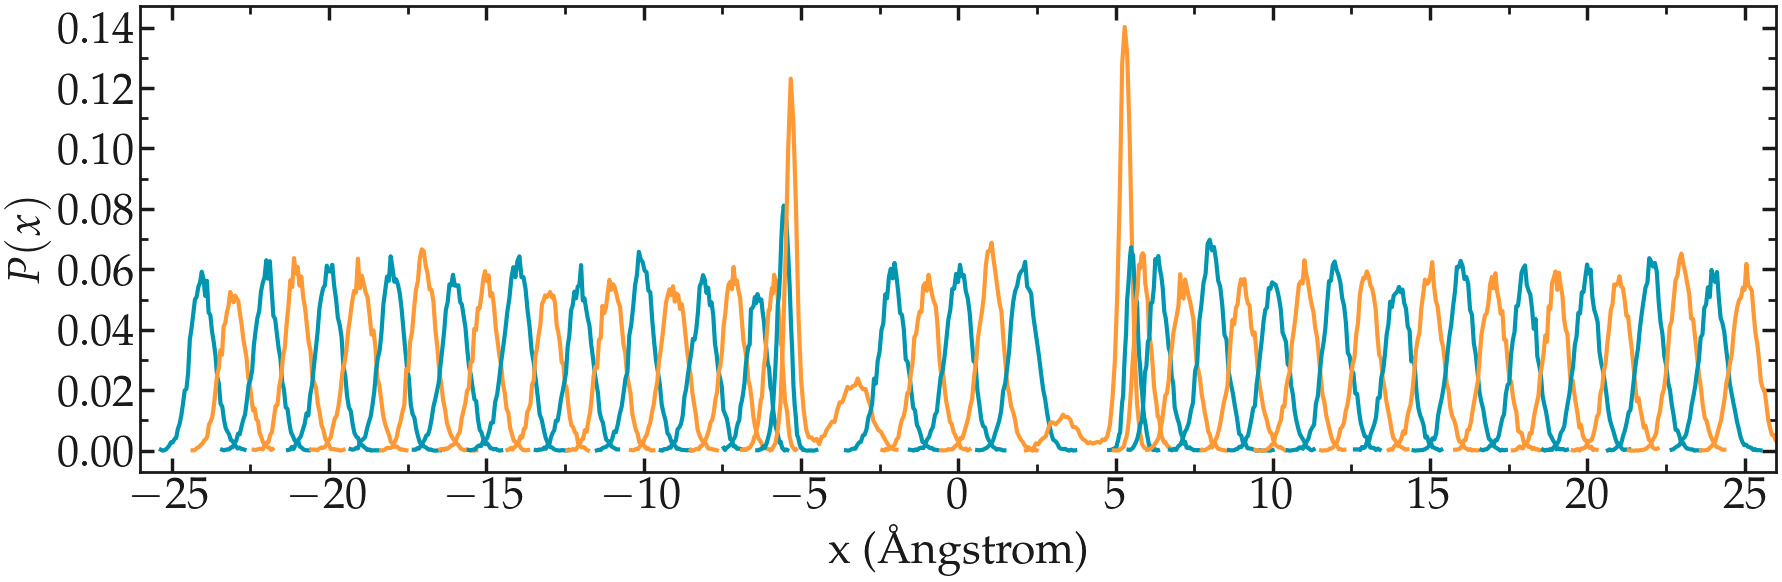
\includegraphics[width=\linewidth]{tutorials/level3/free-energy-calculation/overlap-light.png}
\end{figure}

If $k$ is too small, the biasing potential is too weak to force the particle to explores the 
region of interest, making it impossible to reconstruct the PMF:

\begin{figure}
\includegraphics[width=\linewidth]{tutorials/level3/free-energy-calculation/overlap015-light.png}
\end{figure}

If $k$ is too large, the biasing potential is too large 
compared to the potential one want to probe, which reduces the 
sensitivity of the method. In that case, note the bad overlap between neighbor windows:

\begin{figure}
\includegraphics[width=\linewidth]{tutorials/level3/free-energy-calculation/overlap15-light.png}
\end{figure}

\section{Going further with exercises}

\noindent \subsection{The binary fluid that wont mix}

1 - Create the system\textit{}
Create a molecular simulation with two species of respective types 1 and 2.
Apply different potentials $U1$ and $U2$ on particles of types 1 and 2, respectively,
so that particles of type 1 are excluded from the center of the box, while at the same time particles
of type 2 are excluded from the rest of the box, as seen here:

\begin{figure}
\includegraphics[width=\linewidth]{tutorials/level3/free-energy-calculation/exercice2-light.png}
\end{figure}

\begin{tcolorbox}[colback=mylightblue!5!white,colframe=mylightblue!75!black,title=Solution]

\begin{lcverbatim}

group t1 type 1
variable U1 atom ${U0}*atan((x+${x0})/${dlt})-${U0}*atan((x-${x0})/${dlt})
variable F1 atom ${U0}/((x-${x0})^2/${dlt}^2+1)/${dlt}-${U0}/((x+${x0})^2/${dlt}^2+1)/${dlt}
fix myadf1 t1 addforce v_F1 0.0 0.0 energy v_U1
fix_modify myadf1 energy yes
group t2 type 2
variable U2 atom -${U0}*atan((x+${x0})/${dlt})+${U0}*atan((x-${x0})/${dlt})
variable F2 atom -${U0}/((x-${x0})^2/${dlt}^2+1)/${dlt}+${U0}/((x+${x0})^2/${dlt}^2+1)/${dlt}
fix myadf2 t2 addforce v_F2 0.0 0.0 energy v_U2
fix_modify myadf2 energy yes
\end{lcverbatim}

\noindent \begin{lcverbatim}
mass * 39.95
pair_coeff * * ${epsilon} ${sigma}
\end{lcverbatim}

\noindent \end{tcolorbox}

2 - Measure the PMFs\textit{}
Using the same protocole as the one used in the tutorial (i.e. umbrella sampling with the wham algorithm),
extract the PMF for each particle type:

\begin{figure}
\includegraphics[width=\linewidth]{tutorials/level3/free-energy-calculation/exercice-binary-light.png}
\end{figure}

\subsection{Particles under convection}

\noindent Use a similar simulation as the one from the tutorial, with a repulsive potential in the center
of the box. Add a forcing to the particles and force them to flow in the $x$ direction.
Re-measure the potential in presence of the net convection of particles. You should see the 
potential getting tilted as a consequence of the additional force that makes it easier for 
the particles to cross the potential in one of the direction. The barrer will also 
reduced. 

\begin{figure}
\includegraphics[width=\linewidth]{tutorials/level3/free-energy-calculation/exercice-convection-light.png}
\end{figure}

\begin{tcolorbox}[colback=mylightblue!5!white,colframe=mylightblue!75!black,title=Solution]

\begin{lcverbatim}
fix myconv all addforce 2e-6 0 0
\end{lcverbatim}

\noindent \end{tcolorbox}

\subsection{Surface adsorption of a molecule}

\noindent Apply umbrella sampling to calculate the free energy profile
of ethanol in the direction normal to a crystal solid surface (here made of sodium chloride). 
Find the \href{../../../../../inputs/level3/free-energy-calculation/Exercises/MoleculeAdsorption/system/}{topology files}, \href{../../../../../inputs/level3/free-energy-calculation/Exercises/MoleculeAdsorption/PARM.lammps}{parameter file}, and a \href{../../../../../inputs/level3/free-energy-calculation/Exercises/MoleculeAdsorption/input-minimalist.lammps}{minimal input file}.
The PMF normal to a wall indicates the free energy of adsorption, which is
calculated from the difference between the PMF far from the surface, and the 
PMF at the wall.

\begin{figure}
\includegraphics[width=\linewidth]{tutorials/level3/free-energy-calculation/ethanol-light.png}
\end{figure}

The PMF looks like that, with the position of the wall being near $x=0$.
The PMF mimina near the solid surface indicates the good affinity of the wall with 
the molecule.

\begin{figure}
\includegraphics[width=\linewidth]{tutorials/level3/free-energy-calculation/exercice-ethanol-light.png}
\end{figure}

Alternatively to using ethanol, feel free to download the molecule of your choice, for 
instance from the  Automated Topology Builder (ATB). You will make your life simpler
by choosing one small molecule, like for instance CO2, a small alcohol, water, etc.


\include{non-tutorials/solutions.tex}
\include{tutorials/vmd/vmd-tutorial.tex}
\include{tutorials/mdanalysis/mda-tutorial.tex}

\end{document}

